% do not change these two lines (this is a hard requirement
% there is one exception: you might replace oneside by twoside in case you deliver 
% the printed version in the accordant format
\documentclass[11pt,titlepage,oneside,openany]{book}
\usepackage{times}


\usepackage{graphicx}
\usepackage{latexsym}
\usepackage{amsmath}
\usepackage{amssymb}

\usepackage{ntheorem}

% \usepackage{paralist}
\usepackage{tabularx}

% this packaes are useful for nice algorithms
\usepackage{algorithm}
\usepackage{algorithmic}

\usepackage[shortlabels]{enumitem}
\usepackage{hyperref}
\hypersetup{
    pdftitle={Master Thesis},
    pdfauthor={Lars Joormann},
    colorlinks=false,
    pdfborder={0 0 0},
    }
\usepackage{longtable}

\urlstyle{same}

% well, when your work is concerned with definitions, proposition and so on, we suggest this
% feel free to add Corrolary, Theorem or whatever you need
\newtheorem{definition}{Definition}
\newtheorem{proposition}{Proposition}


% its always useful to have some shortcuts (some are specific for algorithms
% if you do not like your formating you can change it here (instead of scanning through the whole text)
\renewcommand{\algorithmiccomment}[1]{\ensuremath{\rhd} \textit{#1}}
\def\MYCALL#1#2{{\small\textsc{#1}}(\textup{#2})}
\def\MYSET#1{\scshape{#1}}
\def\MYAND{\textbf{ and }}
\def\MYOR{\textbf{ or }}
\def\MYNOT{\textbf{ not }}
\def\MYTHROW{\textbf{ throw }}
\def\MYBREAK{\textbf{break }}
\def\MYEXCEPT#1{\scshape{#1}}
\def\MYTO{\textbf{ to }}
\def\MYNIL{\textsc{Nil}}
\def\MYUNKNOWN{ unknown }
% simple stuff (not all of this is used in this examples thesis
\def\INT{{\mathcal I}} % interpretation
\def\ONT{{\mathcal O}} % ontology
\def\SEM{{\mathcal S}} % alignment semantic
\def\ALI{{\mathcal A}} % alignment
\def\USE{{\mathcal U}} % set of unsatisfiable entities
\def\CON{{\mathcal C}} % conflict set
\def\DIA{\Delta} % diagnosis
% mups and mips
\def\MUP{{\mathcal M}} % ontology
\def\MIP{{\mathcal M}} % ontology
% distributed and local entities
\newcommand{\cc}[2]{\mathit{#1}\hspace{-1pt} \# \hspace{-1pt} \mathit{#2}}
\newcommand{\cx}[1]{\mathit{#1}}
% complex stuff
\def\MER#1#2#3#4{#1 \cup_{#3}^{#2} #4} % merged ontology
\def\MUPALL#1#2#3#4#5{\textit{MUPS}_{#1}\left(#2, #3, #4, #5\right)} % the set of all mups for some concept
\def\MIPALL#1#2{\textit{MIPS}_{#1}\left(#2\right)} % the set of all mips
\newcommand{\norm}[1]{\left\lVert#1\right\rVert}

\newcommand{\cross}[1][1pt]{\ooalign{%
  \rule[1ex]{1ex}{#1}\cr% Horizontal bar
  \hss\rule{#1}{.7em}\hss\cr}}% Vertical bar
\begin{document}

\pagenumbering{roman}
% lets go for the title page, something like this should be okay
\begin{titlepage}
	\vspace*{2cm}
  \begin{center}
   {\Large Comparison of Symbolic \& Sub-Symbolic Approaches for Knowledge Graph Completion\\}
   \vspace{2cm} 
   {Master Thesis\\}
   \vspace{2cm}
   {presented by\\
    Lars Joormann \\
    Matriculation Number 1721931\\
   }
   \vspace{1cm} 
   {submitted to the\\
    Data and Web Science Group\\
    Prof.\ Dr.\ Stuckenschmidt\\
    University of Mannheim\\} \vspace{2cm}
   {August 2022}
  \end{center}
\end{titlepage} 
% no lets make some add some table of contents

\chapter*{Abstract}
\label{cha:abstract}
\textit{Add a brief summary!}

\tableofcontents

\listofalgorithms

\listoffigures

\listoftables

% evntuelly you might add something like this
% \listtheorems{definition}
% \listtheorems{proposition}

\newpage

% okay, start new numbering ... here is where it really starts
\pagenumbering{arabic}

\chapter{Introduction}
\label{cha:intro}
Link Prediction is the task of predicting the existence of a relation between two entities in a knowledge graph. To solve the task a link prediction model exploits the knowledge from the existing links in a knowledge graph to infer missing ones. 

Current research is mainly concerned with sub-symbolic approaches to solve the problem. Here latent representations of the entities and relations of a knowledge graph are learned and applied to an equation in order to calculate predictions about missing links. Popular models from this approach include TransE \cite{bordes_translating_2013}, ComplEx \cite{trouillon_complex_2016} and ConvE \cite{dettmers_convolutional_2018}.   

As an alternative the symbolic approach has attracted much less attention. \cite{wang_knowledge_2017} Models from this approach learn knowledge in a symbolic language from an existing knowledge graph. Often in form of rules. The learned knowledge then can be applied to generate predictions for the task at hand. Models from this approach include AMIE \cite{galarraga_amie_2013}, AnyBURL \cite{meilicke_anytime_2019} and RLvLR \cite{ghiasnezhad_omran_scalable_2018}. Here especially AnyBURL delivers result competitive to the sub-symbolic approaches. 

\section{Motivation}
In this master thesis I want to compare the results of symbolic and sub-symbolic approaches on commonly used datasets e.g. Codex \cite{safavi_codex_2020}, FB15k-237 \cite{toutanova_observed_2015} and WNRR \cite{dettmers_convolutional_2018}. Usually the performance of models are compared by calculating an aggregated metric over the results for the test dataset e.g. mean reciprocal rank or hits@k. I plan to do the comparison in a more granular approach. The goal here is to determine whether subsets of the datasets exists which share a common characteristic where one approach significantly outperforms the other. 

If I am able to identify subsets which satisfy this criteria this found knowledge could help to deepen our understanding of the strengths and weaknesses of symbolic and sub-symbolic approaches and could open the opportunity  to create hybrid models which combine the advantages of both approaches.

\section{Research Questions}
\label{sec:research_questions}
The main research question of this work is: Are there patterns in subsets of a dataset where one approach (symbolic or sub-symbolic) outperforms the other? 
Subsets here are created from the test data and divided by characteristics of the included triples. I plan on investigating following characteristics:

\begin{enumerate}[(i)]
\item Relation Class
\item Relation Frequency in the Trainings Data
\item Entity Frequency in the Trainings Data
\item Existence of Similar Triples in the Trainings Data
\item Existence of Similar Entities in the Dataset
\end{enumerate}

Furthermore, if such subsets exist another question I plan to answer is, if these sets can be used to test models for vulnerabilities in specific areas e.g. to test whether a model has problems handling less frequent entities. 

\section{Thesis Structure}
The remainder of this thesis is structured as follows. Chapter \ref{cha:knowledge_graphs} and \ref{cha:knowledge_graph_completion} outline the theoretical background, first chapter \ref{cha:knowledge_graphs} discusses what knowledge graphs are in general and for what they are usually utilized. Afterwards, chapter \ref{cha:knowledge_graph_completion} further defines what link prediction is, how symbolic and sub-symbolic approaches differ and presents the models and datasets used in the following analysis. Next, in chapter \ref{cha:experiment_setting} the decisions around the experiments executed to obtain data, used for the analysis in chapter \ref{cha:comparison}, are discussed. In chapter \ref{cha:comparison} the data is then analysed based on the characteristics presented in section \ref{sec:research_questions}. With the results of the comparison testsets, to answer the second research question, are created and evaluated in chapter \ref{cha:testsets}. Chapter \ref{cha:limitations} discusses the research limitations and points out where to expand my research in the future and finally chapter \ref{cha:conclusion} concludes this thesis.
\chapter{Knowledge Graphs}
\label{cha:knowledge_graphs}

Knowledge graphs are graph-structured knowledge bases. They store information in the form of relationships between entities. A single information in the graph is referred to as fact. It consist of two entities and a relation between those two. This can be expressed as a triple: $(head, relation, tail)$. Knowledge Graphs are referred to as graphs since their entities can be interpreted as nodes and the relations as labelled and directed edges in a graph. The label here indicates which kind of relation the entities share and the direction indicates which entity is the head entity and which the tail entity i.e. an edge points from the head to the tail. An example for a knowledge graph can be seen in figure \ref{fig:example_kg}. \cite{nickel_review_2015}

\begin{figure}[H]
\centering
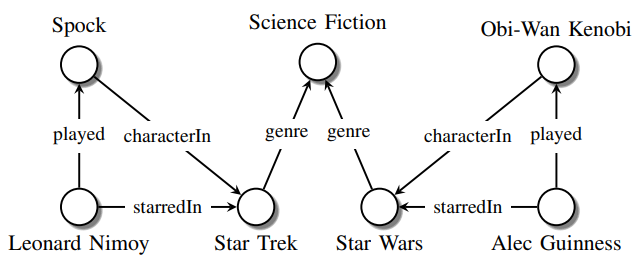
\includegraphics[width=0.9\textwidth]{images/example_kg.png}
\caption{Example of a Knowledge Graph}
\label{fig:example_kg}
\end{figure}

The term 'knowledge graph' was first popularized by Google in 2012 \cite{singhal_introducing_2012}. In their blog they spoke about how they use their knowledge graph to enrich search engine results. The most noticeable part of how they use knowledge graphs are the side windows when searching for an entity with their search engine. An example of such can be seen in figure \ref{fig:side_window_google}. Here we can see what kind of knowledge Google has about the University of Mannheim. For example it seems to be that \textit{(University of Mannheim, founded\_in, 1907)} is one of the facts in their Knowledge Graph.

\begin{figure}[H]
\centering
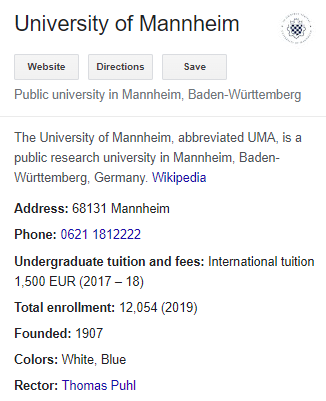
\includegraphics[width=0.5\textwidth]{images/example_google_side_window.png}
\caption{Example of a Google Side Window}
\label{fig:side_window_google}
\end{figure}

In the recent years knowledge graphs have become more and more popular and have found their way into further applications than search engines. An overview of applications can be seen in figure \ref{fig:application_kg}.   Question Answering systems use knowledge graphs to enhance their results. Examples here include social chatbots and digital assistance like Siri. Recommender Systems leverage knowledge graphs as side information to improve and diversify their recommendations.  Moreover, knowledge graphs are also used in information retrieval, domain-specific applications and more. \cite{zou_survey_2020}

\begin{figure}[H]
\centering
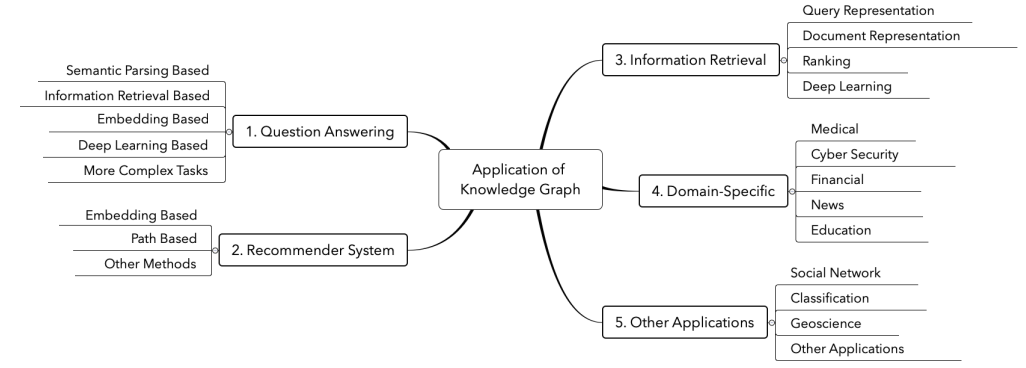
\includegraphics[width=0.9\textwidth]{images/applications_kg.png}
\caption{Applications of Knowledge Graphs}
\label{fig:application_kg}
\end{figure}

According to Paulheim \cite{paulheim_knowledge_2016} a knowledge graph is defined by the following four characteristics: 

\begin{enumerate}
\item "mainly describes real world entities and their interrelations, organized in a graph"
\item "defines possible classes and relations of entities
in a schema"
\item "allows for potentially interrelating arbitrary entities with each other"
\item "covers various topical domains"
\end{enumerate}

The first characteristic defines that knowledge graphs consist of two kind of instances, entities and relations. An entity can be almost everything from an individual person to any kind of object. These entities are then linked through different kind of relations, which forms our graph. 

The schema of the graph plays only a minor role. In most cases the instance-level statements (entities and triples) far outnumber the schema-level statements (entity classes and relations). 

With the third characteristic Paulheim opens up the possibility that there are arbitrary relations between entities which are not included in the knowledge graph. The chapter \ref{cha:knowledge_graph_completion} will discuss this further. 

Lastly, another characteristic of knowledge graphs is that they do not focus on a single domain but interlink multiple topical domains. 
\chapter{Knowledge Graph Completion}
\label{cha:knowledge_graph_completion}

As discussed in section \ref{cha:knowledge_graphs} knowledge graphs are not complete. They contain noisy  and incomplete data. It is practically impossible to cover every possible entity and relation existing in the real-world or even in their domain. There might be missing entities and relations or a Knowledge Graph can include two entities/ relations representing the same real-world entity. Knowledge graph completion tries to tackle these and other problems. It can be seen as a way of data cleaning for knowledge graphs. The solutions to the problems are defined into clear tasks, these include: entity resolution and entity and link prediction approaches. \\

\textbf{Entity Resolution} is according to Talburt "the process of determining whether two [entities] are referring to the same object or to different objects". \cite{talburt_entity_2011} \\ 

\textbf{Entity Prediction} is the task of integrating new entities into the knowledge graphs. These entities are are discovered from other external sources and the knowledge graph includes no information about them. The goal is to find all possible relations this new entity has to the entities already existing in the graph. \cite[p.~1]{baumgartner_entity_2021} \\

\textbf{Link Prediction} is quiet similar to entity prediction. Instead of finding links for a new entity the goal here is to find all missing relations between already existing entities. \cite[p.~125]{golbeck_analyzing_2013} Link prediction can be approached in two different ways: entity classification and triple classification. "Entity classification tries to predict the type or the class of an entity [...]" \cite{ilkou_symbolic_2020} For a triple with a missing tail $(h,r,?)$ the goal would be to list all entities which fit into the tail along with their confidence. Triple classification on the other hand is a binary tasks. Here the input is a compete triple $(h,r,t)$ and the goal is to predict whether this triple is true or not. \cite{ilkou_symbolic_2020} \\

In the following we are going to focus on the task of link prediction. There are various models tackling the problem. They can be categorized into one of the following two categories: symbolic and sub-symbolic approaches. While symbolic methods try to learn an explicit symbolic representation of the patterns found in the knowledge graph, sub-symbolic methods try to solve the problem by learning a latent representation, also often referred to as embeddings, for every entity and relation in the knowledge graph. \cite{meilicke_reinforced_2020} 

\section{Symbolic Approaches}
\label{cha:symbolic_methods}

\subsection{AnyBURL}
\label{cha:anyburl}

\section{Sub-Symbolic Approaches}
\label{cha:sub_symbolic_methods}

Sub-symbolic approaches are based on statistics. They try to learn correlations from the existing triples in the knowledge graph. These can then be expressed as a model which in return allows to predict missing facts.  \cite{nickel_review_2016} The most prominent models of this approach are embedding-based models. These models learn a vector for each entity and relation. The resulting embedding then represents our entity or relation. In this representation it is then assumed that similar entities and similar relations will have similar vectors. An example for these embeddings can be seen in figure \ref{fig:embedding_example}. On the left side we see a knowledge graph with three entities and two relations. Every entity and relation are represented on the right side as an embedding. Our two entities \textit{Washington D.C} and \textit{New York City} are both cities and therefore we can assume that their semantical meaning are quiet similar. The embeddings of these two entities are also quiet similar which demonstrates that our previous assumption is correct. \cite{bianchi_knowledge_2021} Our embeddings are also called latent features because they can not be directly observed in the data. Instead our model has to infer these features from the data. \cite{nickel_review_2016} 

\begin{figure}[H]
\centering
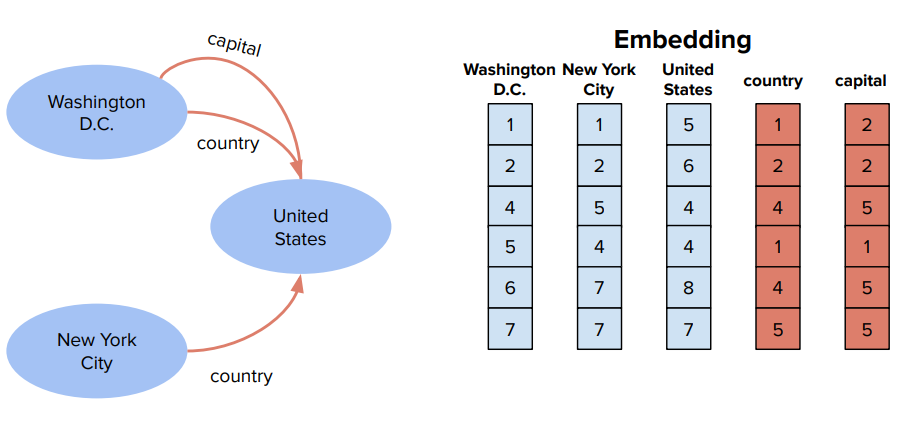
\includegraphics[width=0.9\textwidth]{images/embedding_example.png}
\caption{Example of an Embedding for a Knowledge Graph}
\label{fig:embedding_example}
\end{figure}

An embedding-based model is defined by three characteristics \cite{bianchi_knowledge_2021}:

\begin{enumerate}
\item representations of entities and relationships
\item the scoring function
\item the loss function
\end{enumerate}

As stated earlier our entities and relations are represented through vectors, their embeddings. Some models vary from this a bit and use complex numbers instead of real ones \cite{trouillon_complex_2016}  or use matrices to represent relationships \cite{nickel_three-way_2011}.
\\
The score function $f(h,r,t)$ calculates the distance between the embeddings of two entities relative to their relation. If the triple holds true, its score should be close to $0$. \\
Lastly the loss function defines the objective which is going to be minimized during the training of our model where the embeddings for our entities and relations are learned.

\subsection{ComplEx}
\label{cha:complex}
\subsection{RESCAL}

\section{Comparison of the Approaches}
\label{cha:compare_approaches}

\section{Model Evaluation}
\label{cha:evaluation}
\chapter{Experimental Setting}
\label{cha:experiment_setting}

Before being able to compare the prediction results of both approaches, we need to run experiments with various models to obtain their rankings over different datasets. These rankings will then be compared in the next chapter.

\section{Datasets}
\label{sec:experiment_datasets}
As datasets I first selected CoDEx-M and WN18RR. CoDEx-M was selected because it is a dataset explicitly created for link prediction which leads to it having an appropriate difficulty for the task. Moreover with its 51 relations and 206k triples it seems to have decent size for having enough data to analyse but not taking to much computational power to conduct my experiments. This also what lead me to pick CoDEx-M over the other CoDEx variants (CoDEx-S and CoDEx-L). \cite{safavi_codex_2020}

WN18RR was picked because of its popularity. Furthermore it includes a smaller set of triples than CoDEx-M, only containing 93k and eleven relations. It could be that the smaller size leads to more comprehensible results during the comparison than the larger CoDEx-M. While conducting the analysis it turned out that having the smaller data size lead to it not being very useful for my case therefore I focused more on the other datasets and as a consequence of that only two models were trained for this dataset, as can be seen in table \ref{tab:dataset_models}. More reason why I found WN18RR not very useful for my case will be discussed in chapter \ref{cha:comparison}.

After ruling out WN18RR I still wanted to have a dataset to compare the results I obtained on CoDEx-M. Therefore I decided to include FB15k-237 which similar sized to CoDEx-M but has some flaws which is the reason I initially picked CoDEx-M over FB15k-237. But despite it flaws, FB15k-237 is still often used as a benchmark and most researchers come to the conclusion that it is nevertheless a useful tool. 

Furthermore, I also wanted to run the comparison on one larger dataset and therefore also included YAGO3-10. Because of its size it is quiet expensive computational-wise to run experiments on it and I therefore only used two models on it.

\section{Models}
As for the models I selected AnyBURL as the only model to represent the symbolic approach. Out of the currently published symbolic models, it is the best performing one. To apply this model to the previously mentioned datasets I used the code published on its website\footnote{\href{https://web.informatik.uni-mannheim.de/AnyBURL/}{https://web.informatik.uni-mannheim.de/AnyBURL/ [last accessed: 15.07.2022]}}. The model has a set of hyperparameters to optimize the learning of rules but since no research has been done yet finding the optimal values, I used the recommended default values for these. 
\\ \\
The sub-symbolic approach gets represented by ComplEx and RESCAL. Both models are often used as benchmarks for other models and produce competitive results. These models are to some extend similar as they can both be categorized as multiplicative models, due to the nature of their score function. To include a model which differs more from these two, I later decided to verify my results with ConvE.
 
To run the experiments for the sub-symbolic models LibKGE was used. LibKGE is a library which produces fast and reproducible results for knowledge graph embeddings. \cite{broscheit_libkge_2020} The library also comes with a set of pretrained models and the corresponding configuration file, to reproduce the experiment. I utilized these configuration files to train my models. 

The embbedings for these models are  initialized with random values before they get optimized during the training. This results in slightly different models every time one gets trained, even when the same configuration is being used. To avoid this random factor influencing my comparison I run every experiment for the sub-symbolic models five times and aggregated the results. This is discussed further in the next section.
\\ \\
Table \ref{tab:dataset_models} shows which model was applied to which dataset. As can be seen ConvE and RESCAL were not applied to all datasets, the reason for that was already discussed in section \ref{sec:experiment_datasets}. All configurations and experiment data is reviewable on Github\footnote{\href{https://github.com/LJ171/Thesis}{https://github.com/LJ171/Thesis}}, as well as the results and code for the comparison of the next chapter.


\begin{table}[H]
\centering
\begin{tabular}{l|cccc}
 & \multicolumn{1}{l}{\textbf{CoDEx-M}} & \multicolumn{1}{l}{\textbf{FB15k-237}} & \multicolumn{1}{l}{\textbf{WN18RR}} & \multicolumn{1}{l}{\textbf{YAGO3-10}} \\ \hline
\textbf{AnyBURL} & x & x & x & x \\
\textbf{ComplEx} & x & x & x & x \\
\textbf{ConvE} & x & x &  &  \\
\textbf{RESCAL} & x & x &  & 
\end{tabular}
\caption{Conducted experiments per dataset}
\label{tab:dataset_models}
\end{table}

\section{Data Aggregation}
In this step the data from the symbolic experiments with AnyBURL and the data from the sub-symbolic experiments with LibKGE gets combined. 
\\ \\
LibKGE produces during the prediction of the test dataset a YAML file which contains an entry per triple of the test dataset which contains the triple $(h,r,t)$, the rank (raw \& filtered) and the prediction direction, whether the head or the tail of the triple was predicted. Since the sub-symbolic experiments are repeated five times I combine their results and aggregate the resulting five ranks per triple into an average rank. An example for this can be seen in table \ref{tab:example_libkge}. Furthermore, we can already see within these three examples that the rank for the individual models can differ significantly. As argued in the previous section this is the reason why the sub-symbolic experiments were repeated five times.

\begin{table}[H]
\centering
\begin{tabular}{l|llll}
\textbf{} & \textbf{h} & \textbf{r} & \textbf{t} & \textbf{\begin{tabular}[c]{@{}l@{}}predicted\\ \_head\end{tabular}} \\ \hline
0 & Q73437 & P1412 & Q1860 & False \\
1 & \multicolumn{1}{r}{Q73437} & P1412 & Q1860 & True \\
2 & Q95076 & P106 & Q10798782 & False
\end{tabular}
\newline
\vspace*{1 cm}
\newline
\begin{tabular}{l|llllll}
\textbf{} & \textbf{\begin{tabular}[c]{@{}l@{}}rank\\ \_filtered\\ \_kge\_0\end{tabular}} & \textbf{\begin{tabular}[c]{@{}l@{}}rank\\ \_filtered\\ \_kge\_1\end{tabular}} & \textbf{\begin{tabular}[c]{@{}l@{}}rank\\ \_filtered\\ \_kge\_2\end{tabular}} & \textbf{\begin{tabular}[c]{@{}l@{}}rank\\ \_filtered\\ \_kge\_3\end{tabular}} & \textbf{\begin{tabular}[c]{@{}l@{}}rank\\ \_filtered\\ \_kge\_4\end{tabular}} & \textbf{\begin{tabular}[c]{@{}l@{}}rank\\ \_filtered\\ \_kge\end{tabular}} \\ \hline
0 & 1 & 1 & 1 & 1 & 1 & 1 \\
1 & 1111 & 1649 & 1187 & 108 & 1755 & 1162 \\
2 & 1236 & 1701 & 190 & 357 & 519 & 801
\end{tabular}
\caption{Example of LibKGE ranks for ComplEx on WN18RR}
\label{tab:example_libkge}
\end{table}

The output file from AnyBURL contains three lines per triples. First the triple $(h,r,t)$, second the ranking for the prediction of the head and and lastly the ranking for the prediction of the tail. The ranking is the filtered ranking and contains for each rank the additional information of the confidence AnyBURL assigned to each rank. Here I extract the two ranks for each triple and the corresponding confidence. Since I want to  be able to calculate the difference-$\psi$ from equation \ref{eq:difference_psi}, I extract the confidence AnyBURL assigns to the rank given by the LibKGE model. If we expand table \ref{tab:example_libkge} by this information we end up with table \ref{tab:example_libkge_anyburl}.

\begin{table}[H]
\centering
\begin{tabular}{l|llll}
\textbf{} & \textbf{h} & \textbf{r} & \textbf{t} & \textbf{\begin{tabular}[c]{@{}l@{}}predicted\\ \_head\end{tabular}} \\ \hline
0 & Q73437 & P1412 & Q1860 & False \\
1 & \multicolumn{1}{r}{Q73437} & P1412 & Q1860 & True \\
2 & Q95076 & P106 & Q10798782 & False
\end{tabular}
\newline
\vspace*{1 cm}
\newline
\begin{tabular}{l|llllll}
\textbf{} & \textbf{\begin{tabular}[c]{@{}l@{}}rank\\ \_filtered\\ \_kge\_0\end{tabular}} & \textbf{\begin{tabular}[c]{@{}l@{}}rank\\ \_filtered\\ \_kge\_1\end{tabular}} & \textbf{\begin{tabular}[c]{@{}l@{}}rank\\ \_filtered\\ \_kge\_2\end{tabular}} & \textbf{\begin{tabular}[c]{@{}l@{}}rank\\ \_filtered\\ \_kge\_3\end{tabular}} & \textbf{\begin{tabular}[c]{@{}l@{}}rank\\ \_filtered\\ \_kge\_4\end{tabular}} & \textbf{\begin{tabular}[c]{@{}l@{}}rank\\ \_filtered\\ \_kge\end{tabular}} \\ \hline
0 & 1 & 1 & 1 & 1 & 1 & 1 \\
1 & 1111 & 1649 & 1187 & 108 & 1755 & 1162 \\
2 & 1236 & 1701 & 190 & 357 & 519 & 801
\end{tabular}
\newline
\vspace*{1 cm}
\newline
\begin{tabular}{l|lllll}
\textbf{} & \textbf{\begin{tabular}[c]{@{}l@{}}rank\\ \_filtered\\ \_anyburl\end{tabular}} & \textbf{\begin{tabular}[c]{@{}l@{}}rank\\ \_difference\end{tabular}} & \textbf{\begin{tabular}[c]{@{}l@{}}anyburl\\ \_confidence\\ \_anyburl\end{tabular}} & \textbf{\begin{tabular}[c]{@{}l@{}}anyburl\\ \_confidence\\ \_kge\end{tabular}} & \textbf{\begin{tabular}[c]{@{}l@{}}difference\\ \_psi\end{tabular}} \\ \hline
0 & 1 & 0 & 0.382083 & 0.382083 & 1 \\
1 & 6960 & -5798 & 0.282316 & 0.536634 & 0.526087 \\
2 & 614.0 & 187 & 0.470588 & 0.368421 & 1.277311
\end{tabular}
\caption{Example of LibKGE ranks for ComplEx on WN18RR expanded by the ranks and confidence of AnyBURL}
\label{tab:example_libkge_anyburl}
\end{table}

In this table we can see that difference-$\psi$ and the difference between the ComplEx and AnyBURL rank indicate the same information (which model is better) but while the rank difference let it seem like ComplEx predicted the second triple significantly better than AnyBURL, including the confidence lessens this effect.   
\chapter{Comparison of Symbolic and Sub-Symbolic Performances}
\label{cha:comparison}
\chapter{Test Sets for Vulnerabilities}
\label{cha:testsets}
\chapter{Discussion}
\label{cha:discussion}
\chapter{Research Limitations}
\label{cha:limitations}
\chapter{Conclusion}
\label{cha:conclusion}

\bibliographystyle{plain}
\bibliography{thesis-ref}


\appendix
\chapter{Further Comparison Figures \& Tables}
\section{Metrics of all trained Models}
\label{apppendix:metrics}
\begin{table}[H]
\centering
\begin{tabular}{l|lll|lll}
                     & \multicolumn{3}{c|}{\textbf{CoDEx-M}} & \multicolumn{3}{c}{\textbf{FB15k-237}} \\ \hline
\textbf{Model} &
  \textbf{\begin{tabular}[c]{@{}l@{}}h@1\\ (filtered)\end{tabular}} &
  \textbf{\begin{tabular}[c]{@{}l@{}}h@10\\ (filtered)\end{tabular}} &
  \textbf{\begin{tabular}[c]{@{}l@{}}MRR\\ (filtered)\end{tabular}} &
  \textbf{\begin{tabular}[c]{@{}l@{}}h@1\\ (filtered)\end{tabular}} &
  \textbf{\begin{tabular}[c]{@{}l@{}}h@10\\ (filtered)\end{tabular}} &
  \textbf{\begin{tabular}[c]{@{}l@{}}MRR\\ (filtered)\end{tabular}} \\ \hline
\textbf{AnyBURL}     &            0.313 &     0.412       & 0.285            &  0.238           &            0.501 & 0.322           \\
\textbf{ComplEx (1)} & 0.261       & 0.475      & 0.334      & 0.253       & 0.534       & 0.346      \\
\textbf{ComplEx (2)} & 0.262       & 0.476      & 0.336      & 0.251       & 0.532       & 0.345      \\
\textbf{ComplEx (3)} & 0.260       & 0.479      & 0.335      & 0.253       & 0.534       & 0.345      \\
\textbf{ComplEx (4)} & 0.262       & 0.474      & 0.335      & 0.253       & 0.534       & 0.346      \\
\textbf{ComplEx (5)} & 0.258       & 0.472      & 0.331      & 0.254       & 0.537       & 0.348      \\
\textbf{ConvE (1)}   & 0.231       & 0.457      & 0.309      & 0.246       & 0.522       & 0.337      \\
\textbf{ConvE (2)}   & 0.234       & 0.460      & 0.312      & 0.246       & 0.520       & 0.338      \\
\textbf{ConvE (3)}   & 0.235       & 0.456      & 0.311      & 0.248       & 0.522       & 0.338      \\
\textbf{ConvE (4)}   & 0.233       & 0.456      & 0.310      & 0.246       & 0.522       & 0.338      \\
\textbf{ConvE (5)}   & 0.233       & 0.456      & 0.310      & 0.248       & 0.521       & 0.338      \\
\textbf{RESCAL (1)}  & 0.241       & 0.453      & 0.314      & 0.264       & 0.539       & 0.356      \\
\textbf{RESCAL (2)}  & 0.248       & 0.456      & 0.319      & 0.262       & 0.532       & 0.351      \\
\textbf{RESCAL (3)}  & 0.240       & 0.454      & 0.313      & 0.264       & 0.539       & 0.356      \\
\textbf{RESCAL (4)}  & 0.245       & 0.455      & 0.318      & 0.266       & 0.540       & 0.358      \\
\textbf{RESCAL (5)}  & 0.246       & 0.458      & 0.319      & 0.266       & 0.540       & 0.358     
\end{tabular}
\caption{Hits@1, Hits@10 and MRR of all models trained for CoDex-M and FB15k-237}
\label{tab:metrics_all_codex_fb15l}
\end{table}

\begin{table}[]
\centering
\begin{tabular}{l|lll|lll}
                     & \multicolumn{3}{c|}{\textbf{WN18RR}} & \multicolumn{3}{c}{\textbf{YAGO3-10}} \\ \hline
\textbf{Model} &
  \textbf{\begin{tabular}[c]{@{}l@{}}h@1\\ (filtered)\end{tabular}} &
  \textbf{\begin{tabular}[c]{@{}l@{}}h@10\\ (filtered)\end{tabular}} &
  \textbf{\begin{tabular}[c]{@{}l@{}}MRR\\ (filtered)\end{tabular}} &
  \textbf{\begin{tabular}[c]{@{}l@{}}h@1\\ (filtered)\end{tabular}} &
  \textbf{\begin{tabular}[c]{@{}l@{}}h@10\\ (filtered)\end{tabular}} &
  \textbf{\begin{tabular}[c]{@{}l@{}}MRR\\ (filtered)\end{tabular}} \\ \hline
\textbf{AnyBURL} &   0.495 &           0.553 &         0.479   &           0.559 & 0.629            &                    0.525 \\
\textbf{ComplEx (1)} & 0.438      & 0.544      & 0.474      & 0.464       & 0.672      & 0.540      \\
\textbf{ComplEx (2)} & 0.440      & 0.546      & 0.476      & 0.467       & 0.674      & 0.541      \\
\textbf{ComplEx (3)} & 0.439      & 0.542      & 0.474      & 0.473       & 0.676      & 0.545      \\
\textbf{ComplEx (4)} & 0.436      & 0.542      & 0.472      & 0.455       & 0.670      & 0.533      \\
\textbf{ComplEx (5)} & 0.436      & 0.545      & 0.473      & 0.459       & 0.671      & 0.534      \\
\textbf{ConvE (1)}   & - & - & - & - & - & -            \\
\textbf{ConvE (2)}   & - & - & - & - & - & -           \\
\textbf{ConvE (3)}   & - & - & - & - & - & -            \\
\textbf{ConvE (4)}   & - & - & - & - & - & -           \\
\textbf{ConvE (5)}   & - & - & - & - & - & -          \\
\textbf{RESCAL (1)}  & - & - & - & - & - & -        \\
\textbf{RESCAL (2)}  & - & - & - & - & - & -       \\
\textbf{RESCAL (3)}  & - & - & - & - & - & -         \\
\textbf{RESCAL (4)}  & - & - & - & - & - & -         \\
\textbf{RESCAL (5)}  & - & - & - & - & - & -        
\end{tabular}
\caption{Hits@1, Hits@10 and MRR of all models trained for WN18RR and YAGO3-10}
\label{tab:metrics_all_wnrr_yago}
\end{table}
\section{Comparison of Rankings for all Models and Datasets}
\label{appendix:rankings}

\subsection{CoDEx-M}

\begin{figure}[H]
\centering
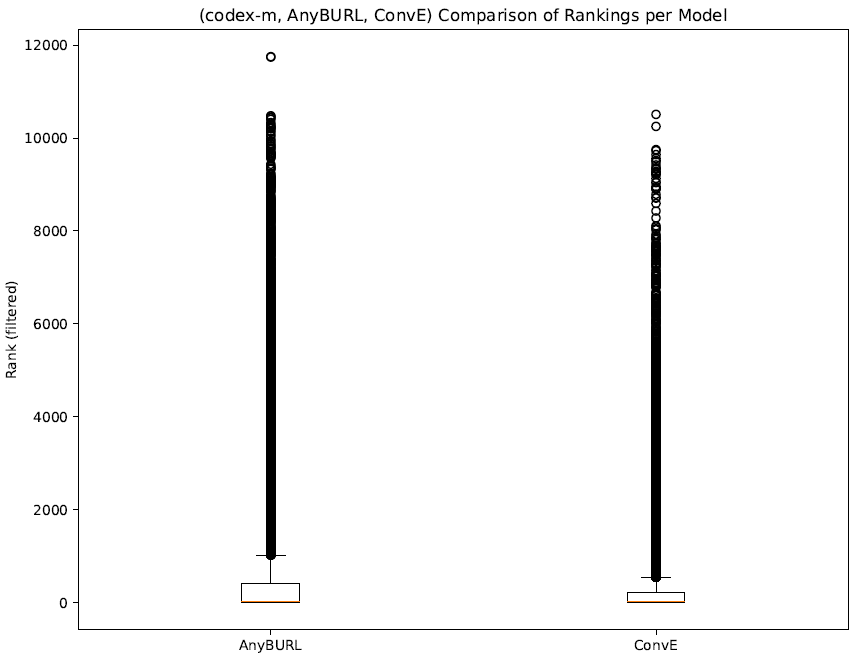
\includegraphics[width=0.8\textwidth]{images/ranks_anyburl_conve_codex.png}
\caption{Comparison of Ranks predicted by AnyBURL and ConvE for CoDEx-M}
\label{fig:ranks_anyburl_conve_codex}
\end{figure}

\begin{figure}[H]
\centering
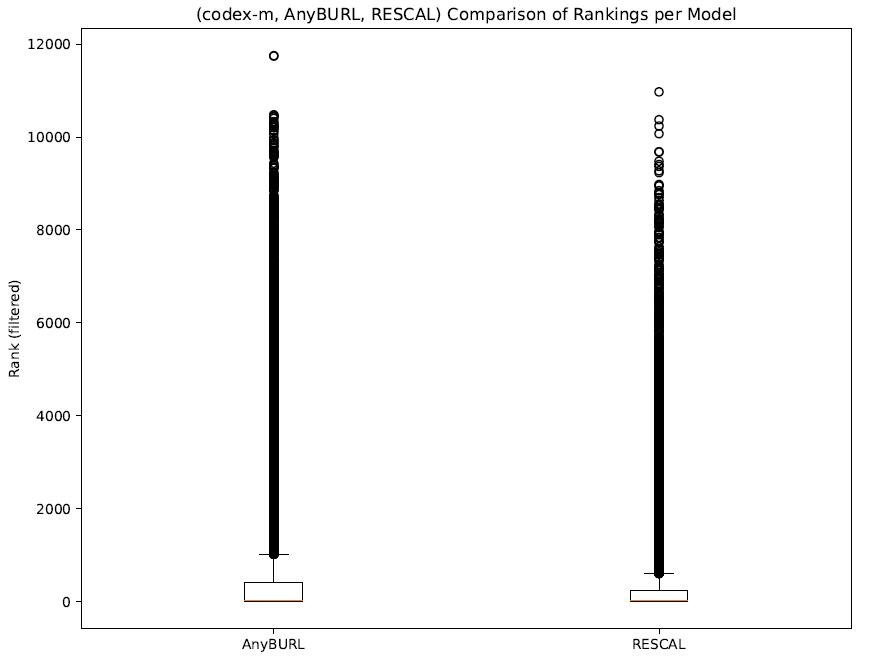
\includegraphics[width=0.8\textwidth]{images/ranks_anyburl_rescal_codex.png}
\caption{Comparison of Ranks predicted by AnyBURL and RESCAL for CoDEx-M}
\label{fig:ranks_anyburl_rescal_codex}
\end{figure}

\subsection{FB15k-237}

\begin{figure}[H]
\centering
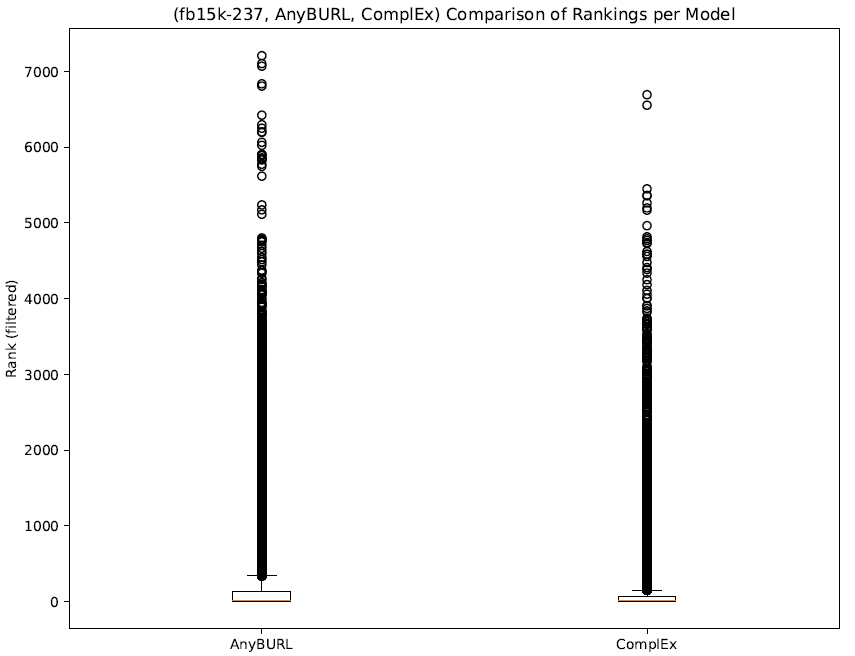
\includegraphics[width=0.8\textwidth]{images/ranks_anyburl_complex_fb15k.png}
\caption{Comparison of Ranks predicted by AnyBURL and ComplEx for FB15k-237}
\label{fig:ranks_anyburl_complex_fb15k}
\end{figure}

\begin{figure}[H]
\centering
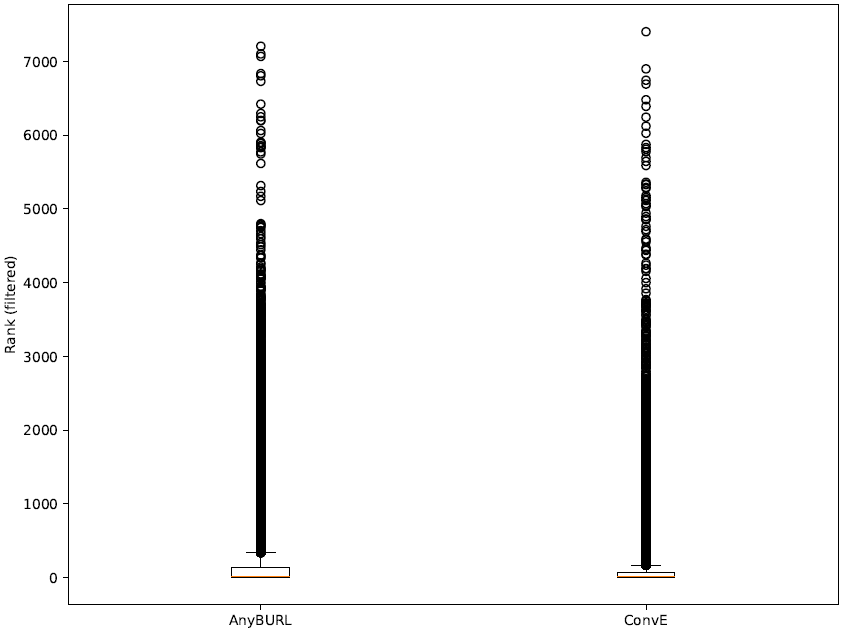
\includegraphics[width=0.8\textwidth]{images/ranks_anyburl_conve_fb15k.png}
\caption{Comparison of Ranks predicted by AnyBURL and ConvE for FB15k-237}
\label{fig:ranks_anyburl_conve_fb15k}
\end{figure}

\begin{figure}[H]
\centering
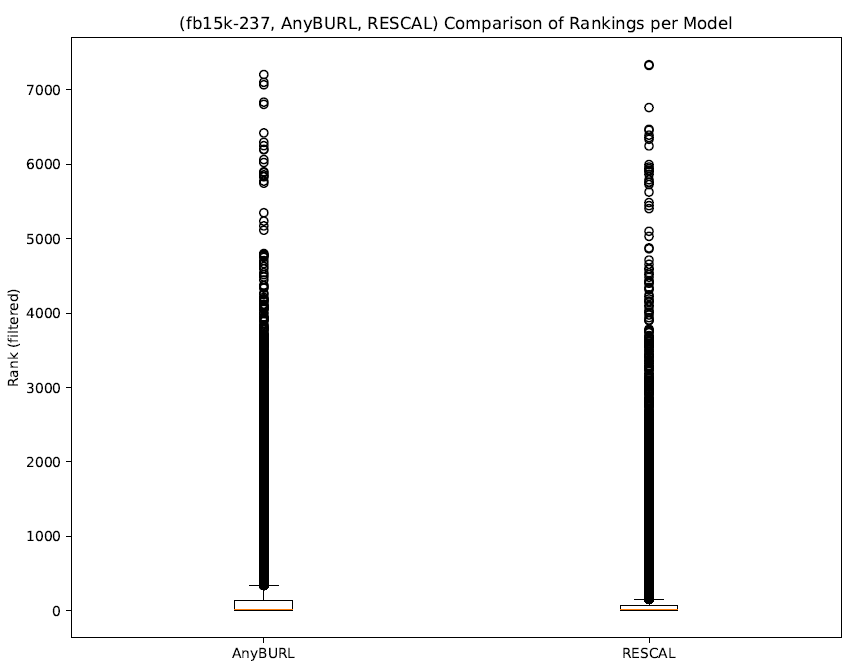
\includegraphics[width=0.8\textwidth]{images/ranks_anyburl_rescal_fb15k.png}
\caption{Comparison of Ranks predicted by AnyBURL and RESCAL for FB15k-237}
\label{fig:ranks_anyburl_rescal_fb15k}
\end{figure}

\subsection{YAGO3-10}

\begin{figure}[H]
\centering
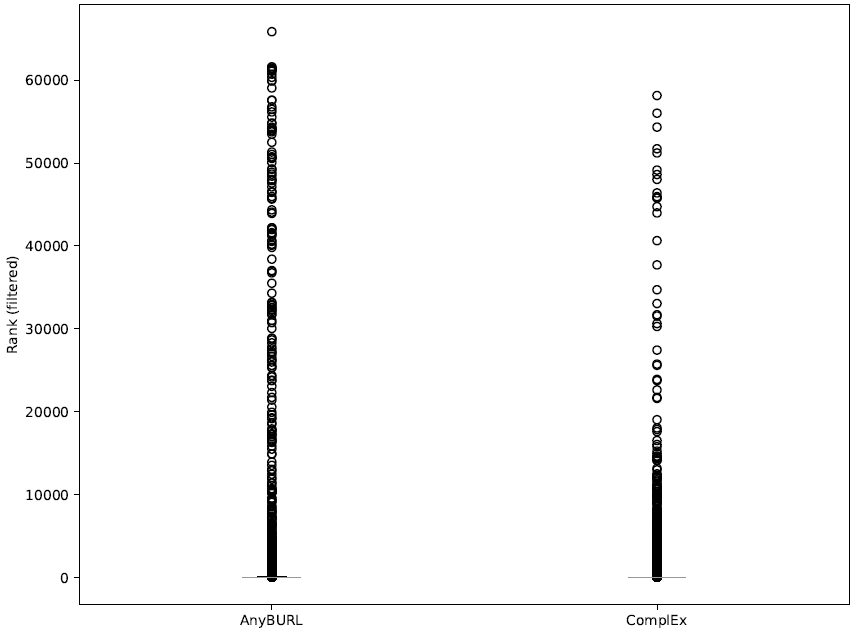
\includegraphics[width=0.8\textwidth]{images/ranks_anyburl_complex_yago.png}
\caption{Comparison of Ranks predicted by AnyBURL and ComplEx for YAGO3-10}
\label{fig:ranks_anyburl_complex_yago}
\end{figure}
\section{Comparison in regard to the Relation Classes}
\label{appendix:relation_class_fb15k}

\begin{figure}[H]
\centering
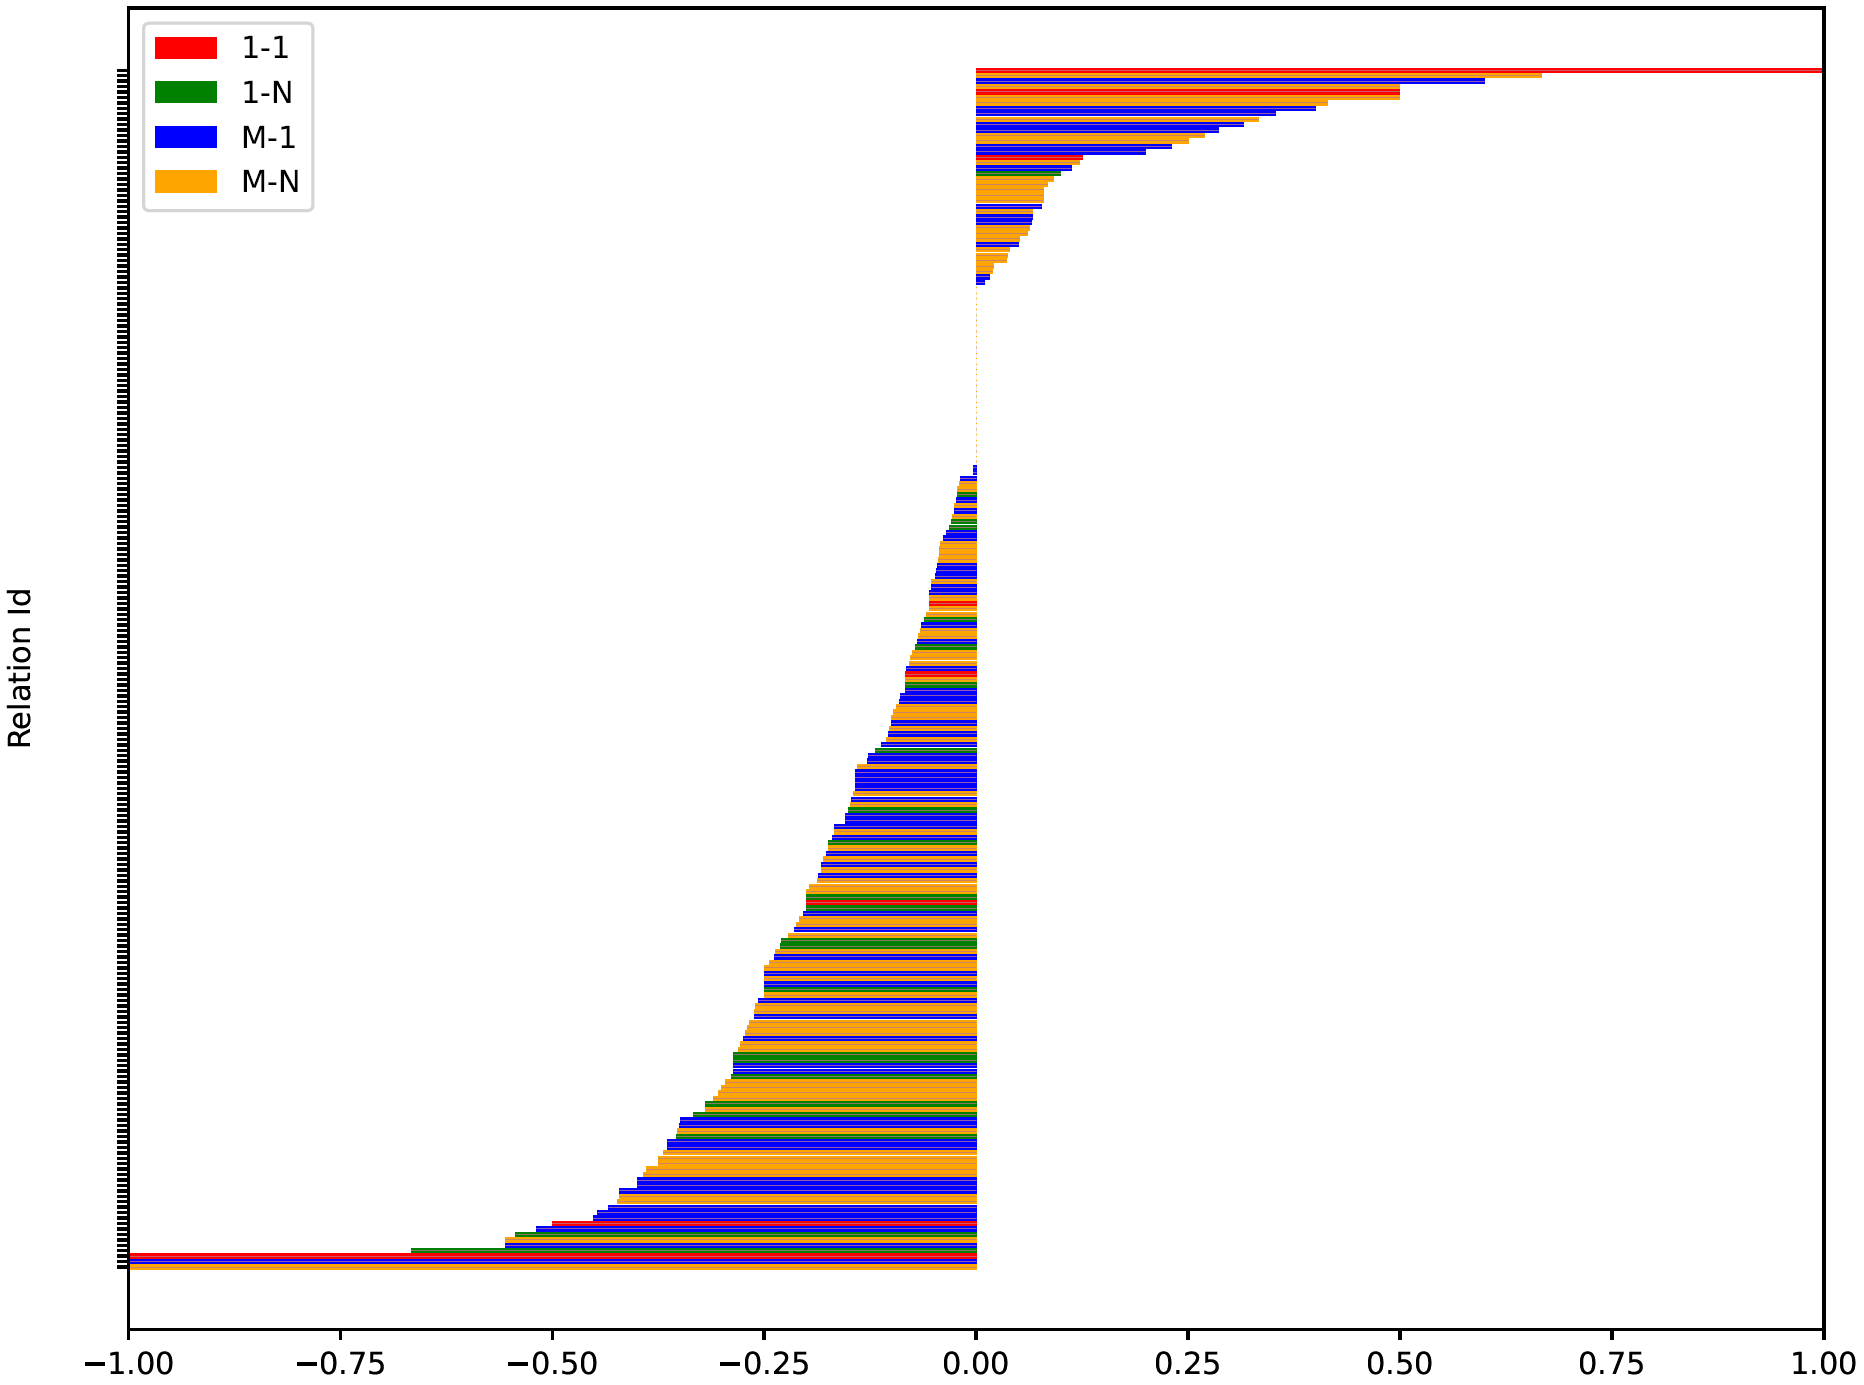
\includegraphics[width=0.7\textwidth]{images/relation_class_anyburl_complex_fb15k.PNG}
\caption{Comparison of AnyBURL and ComplEx on FB15k-237 in regard to the relation classes}
\label{fig:relation_class_anyburl_complex_fb15k}
\end{figure}

\begin{figure}[H]
\centering
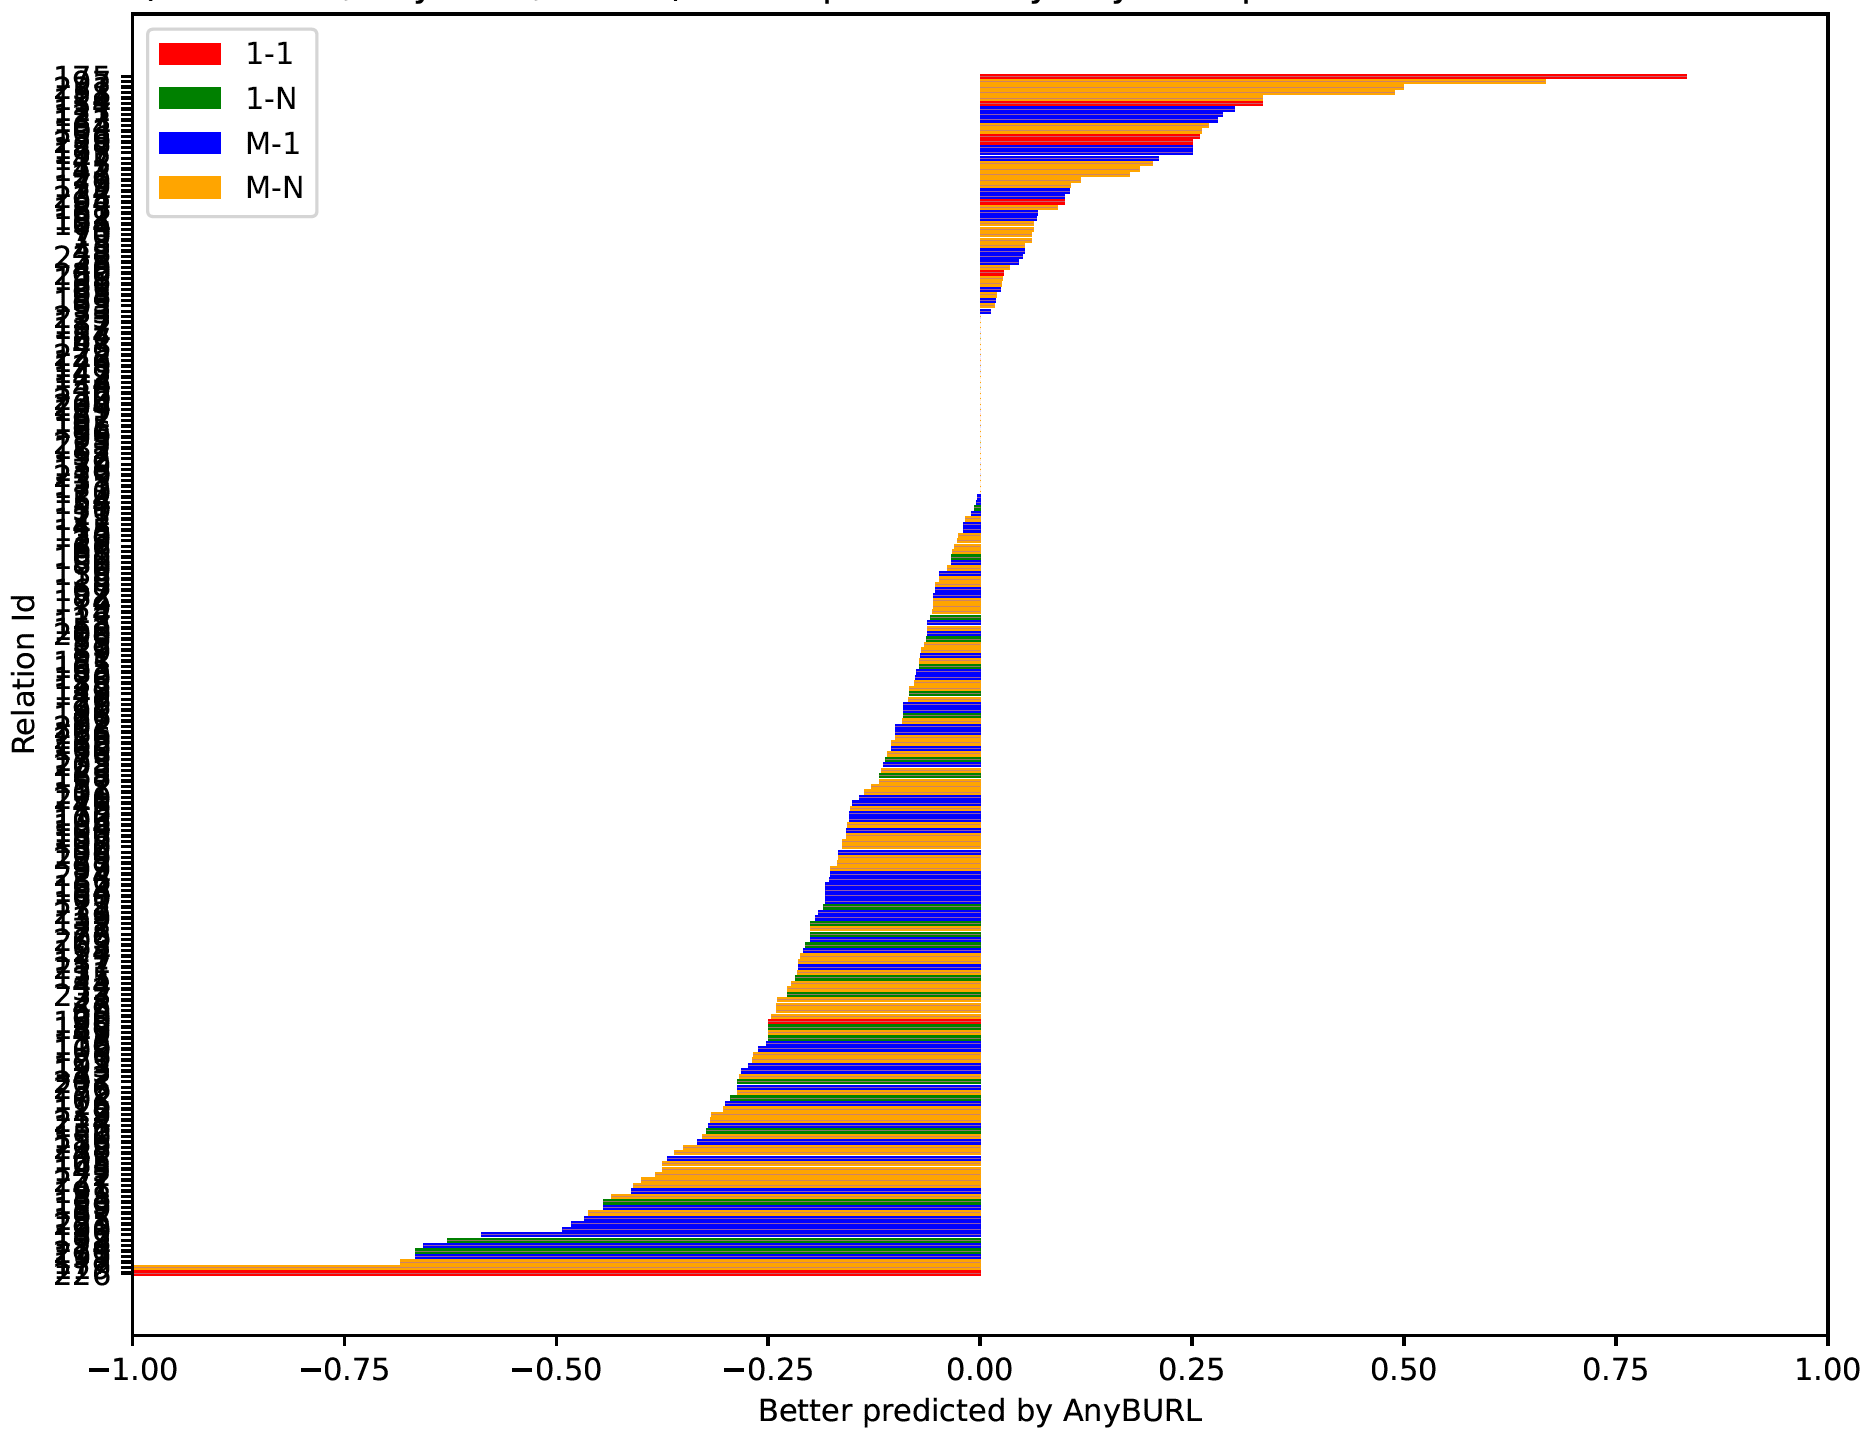
\includegraphics[width=0.7\textwidth]{images/relation_class_anyburl_conve_fb15k.PNG}
\caption{Comparison of AnyBURL and ConvE on FB15k-237 in regard to the relation classes}
\label{fig:relation_class_anyburl_conve_fb15k}
\end{figure}

\begin{figure}[H]
\centering
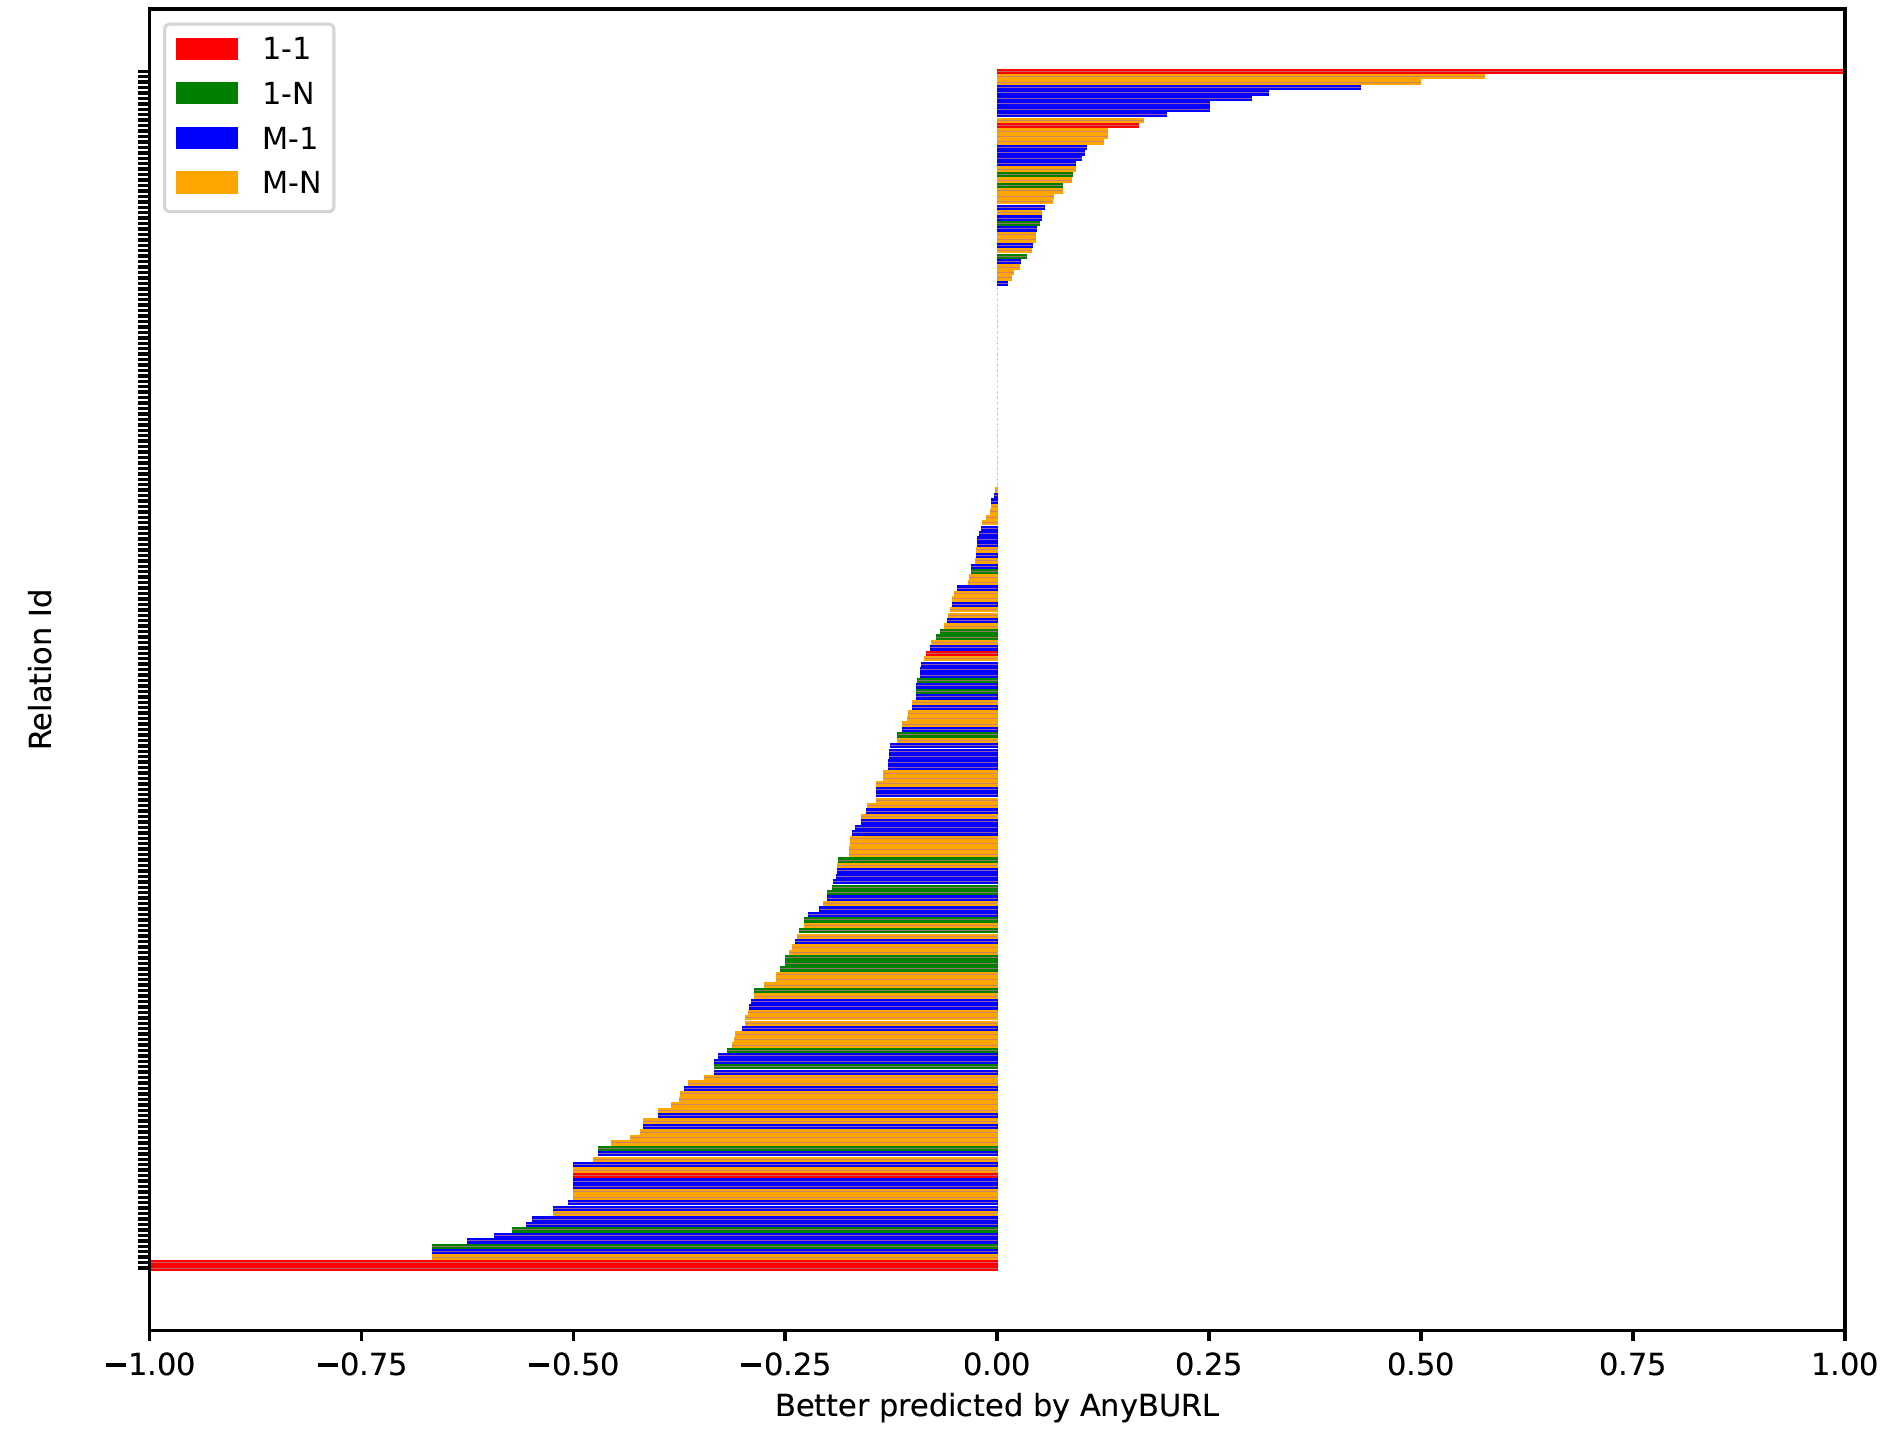
\includegraphics[width=0.7\textwidth]{images/relation_class_anyburl_rescal_fb15k.PNG}
\caption{Comparison of AnyBURL and RESCAL on FB15k-237 in regard to the relation classes}
\label{fig:relation_class_anyburl_rescal_fb15k}
\end{figure}
\section{Relation Frequency in Trainings Data}
\label{appendix:relation_freq}

\begin{figure}[H]
\centering
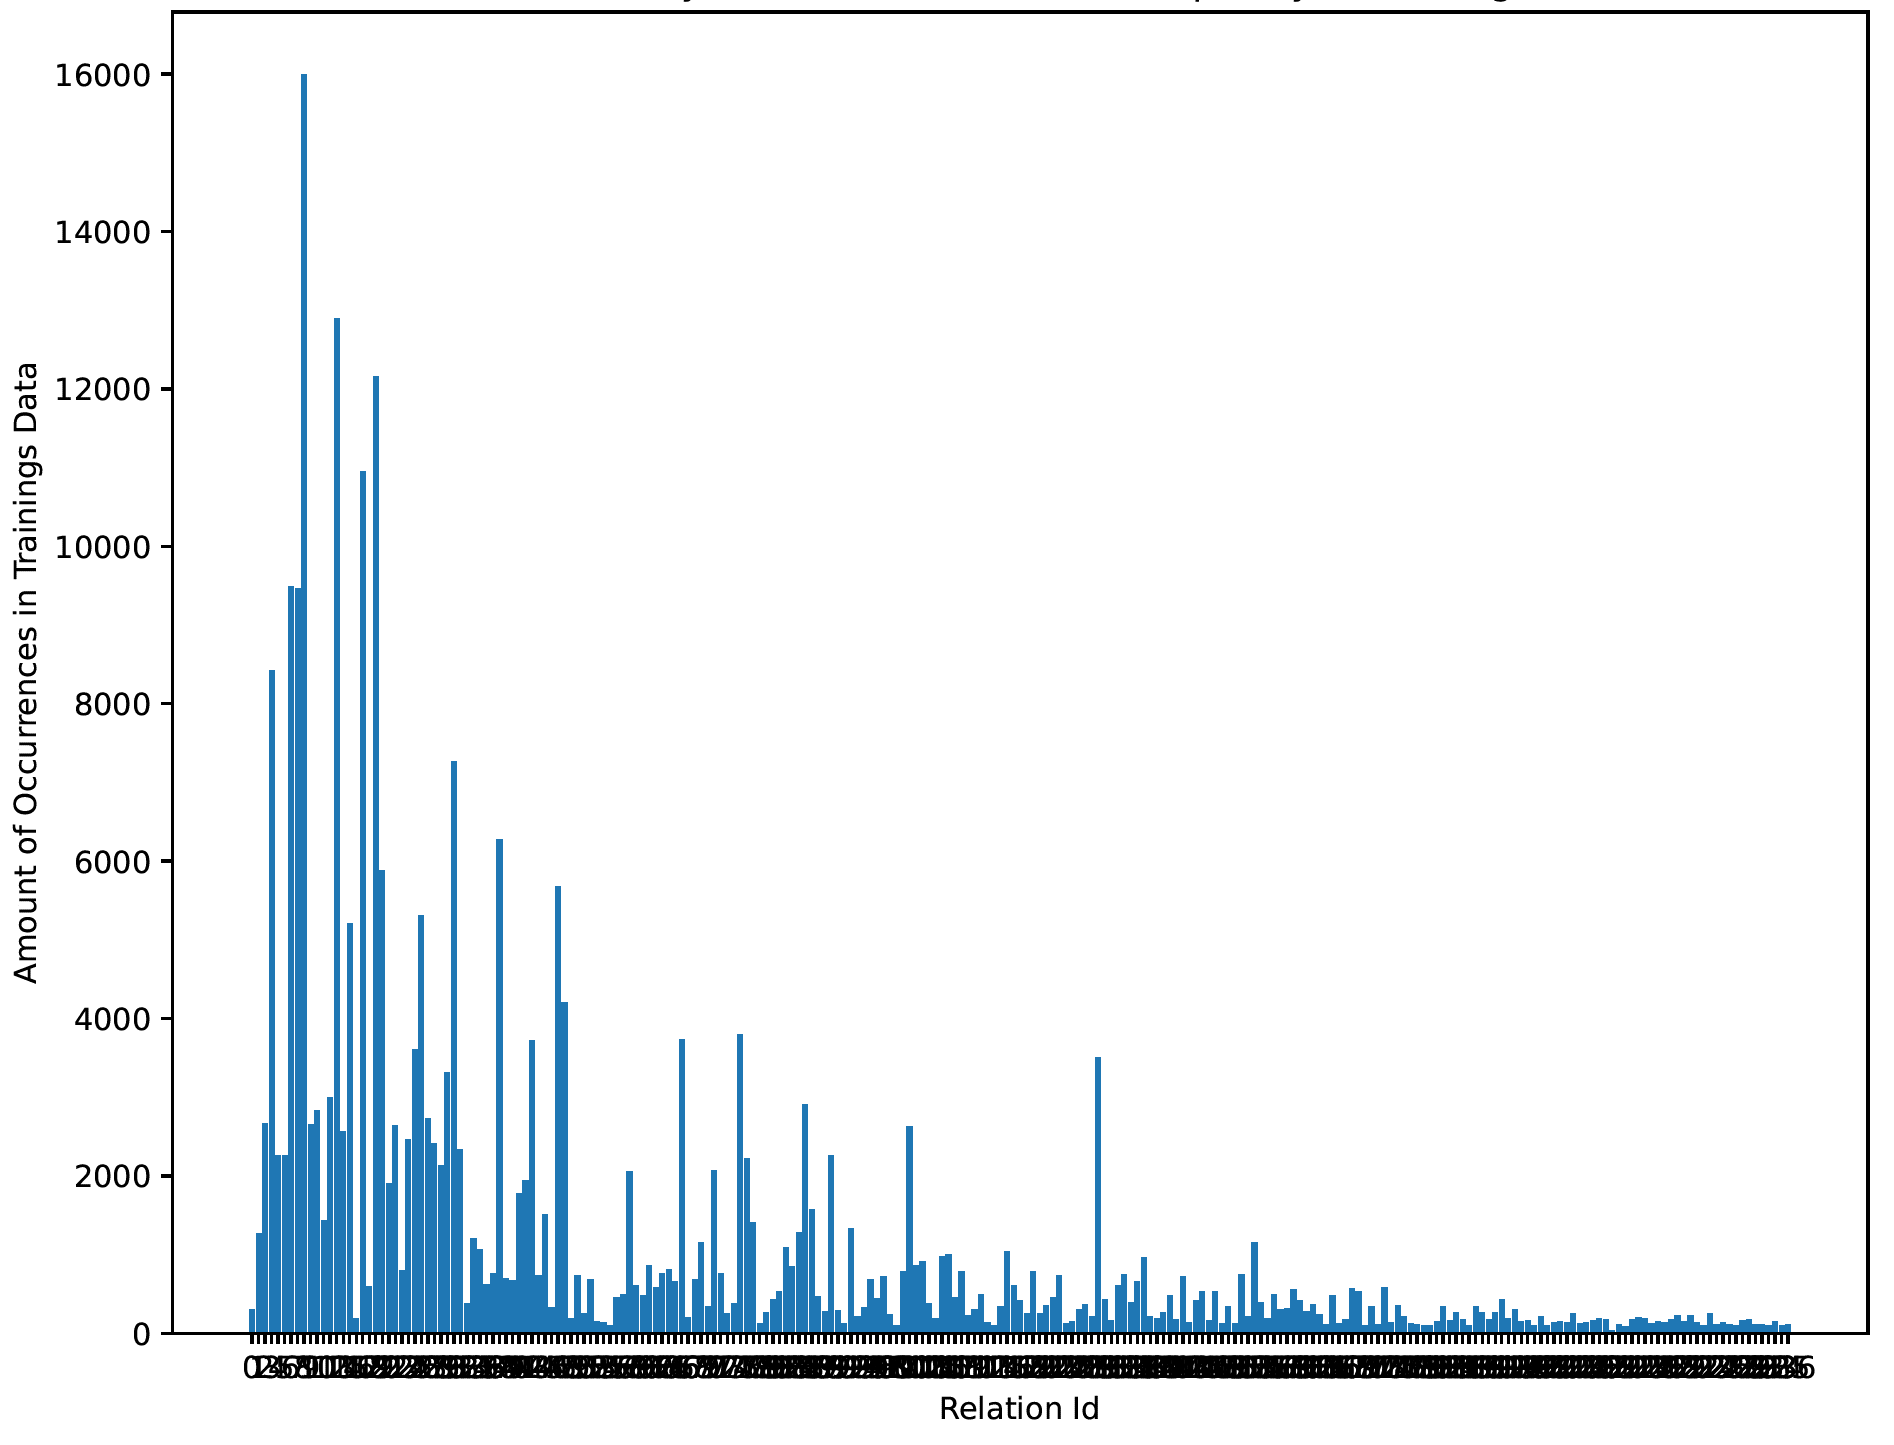
\includegraphics[width=0.7\textwidth]{images/relation_freq_fb15k.PNG}
\caption{Relation frequency in trainings data for FB15k-237}
\label{fig:relation_freq_fb15k}
\end{figure}

\begin{figure}[H]
\centering
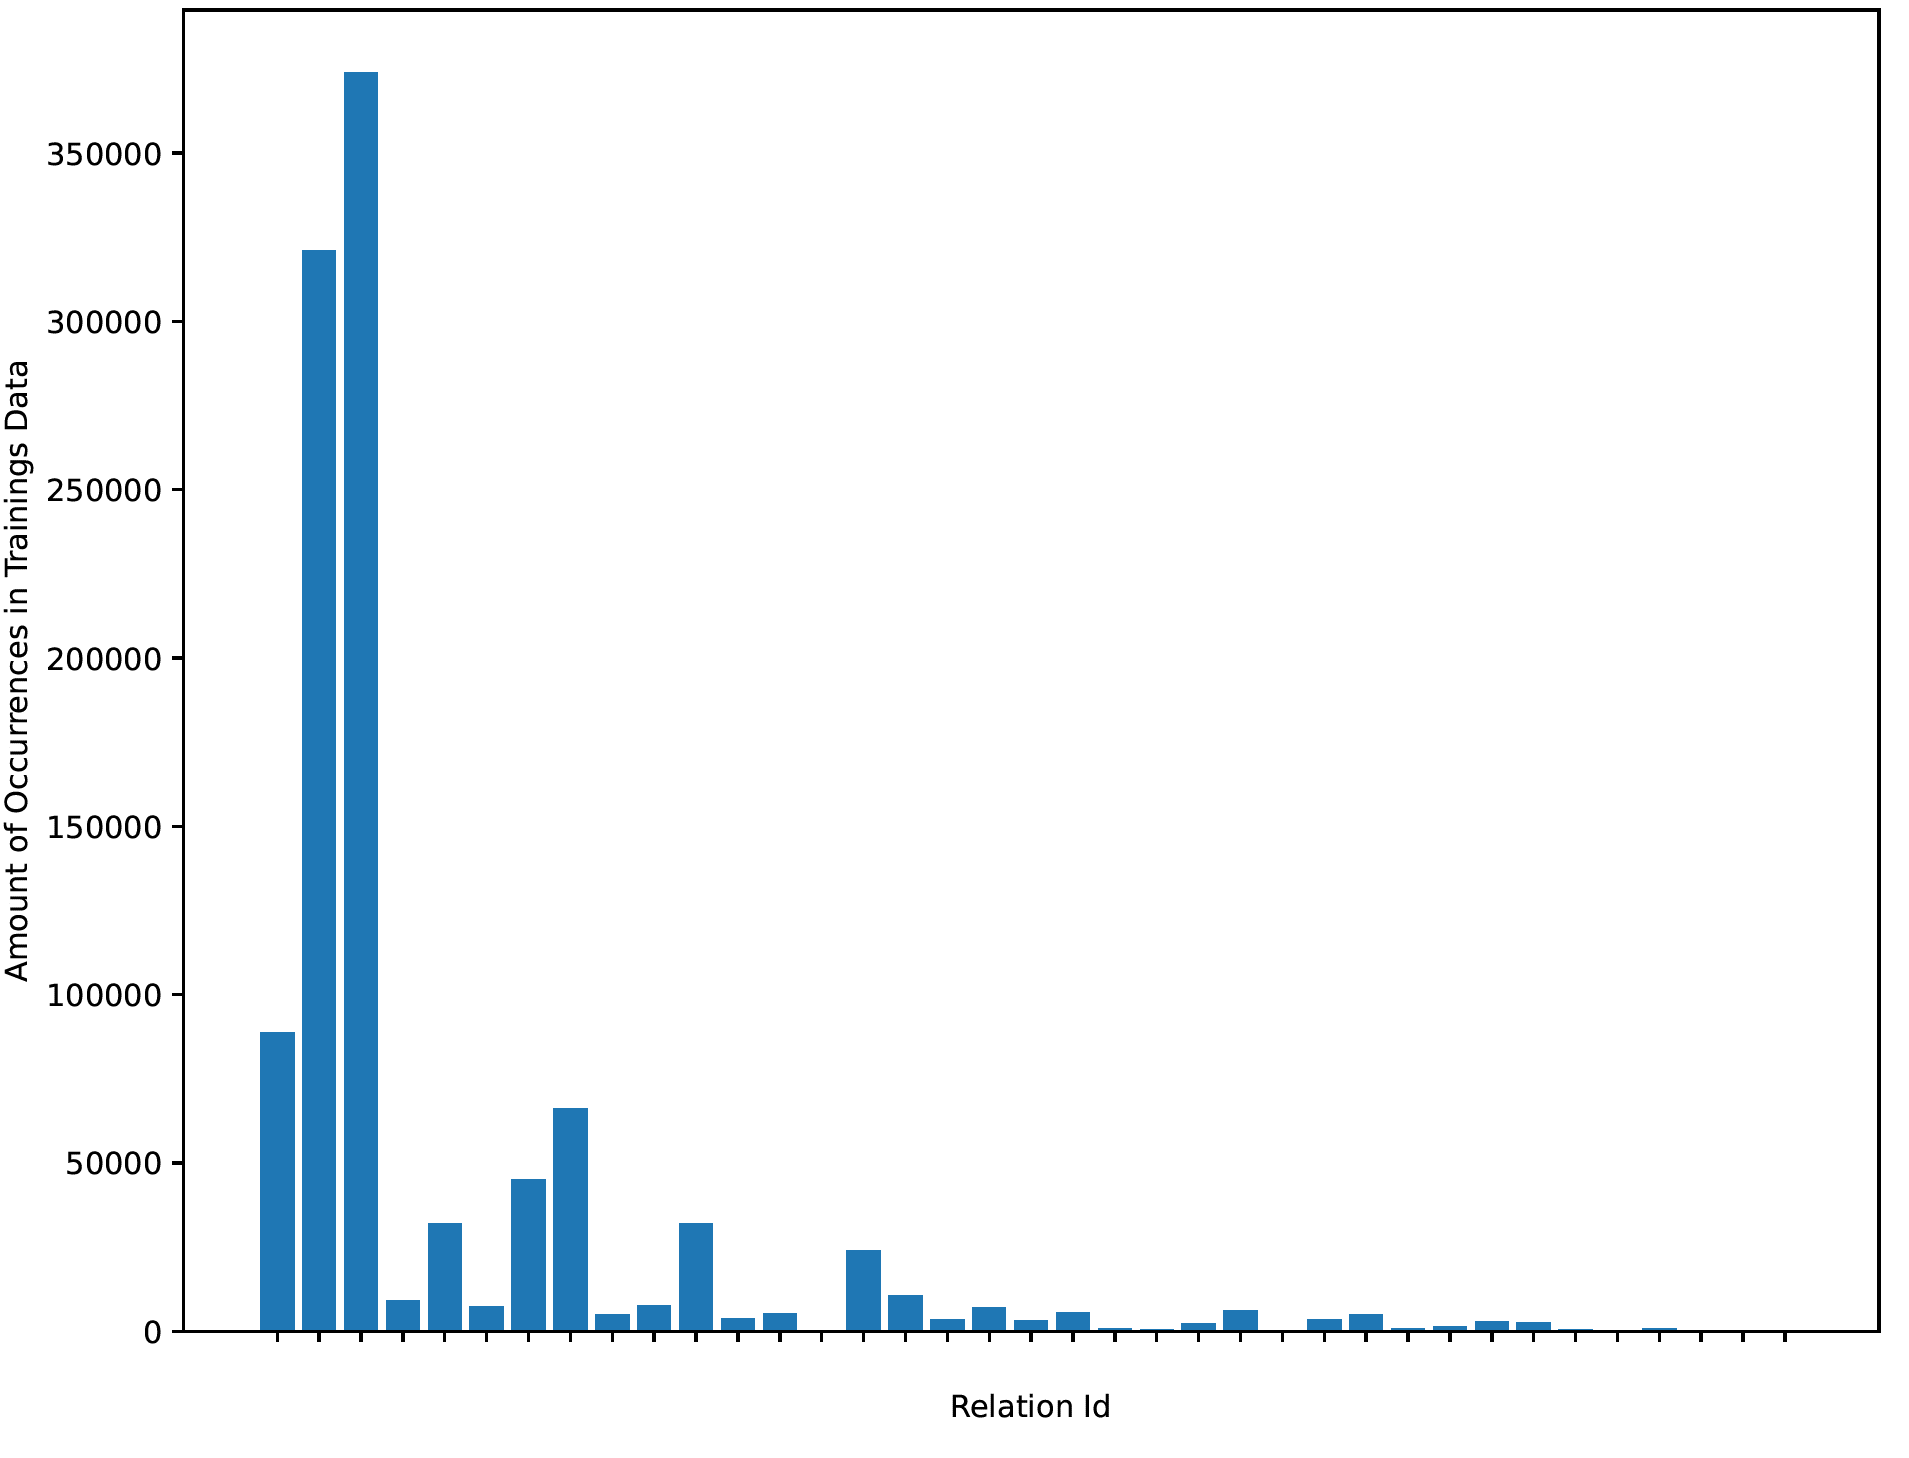
\includegraphics[width=0.7\textwidth]{images/relation_freq_yago.PNG}
\caption{Relation frequency in trainings data for YAGO3-10}
\label{fig:relation_freq_yago}
\end{figure}
\section{Comparison in regard to the Relation Frequency}
\label{appendix:relation_freq_fb15k}

\begin{figure}[H]
\centering
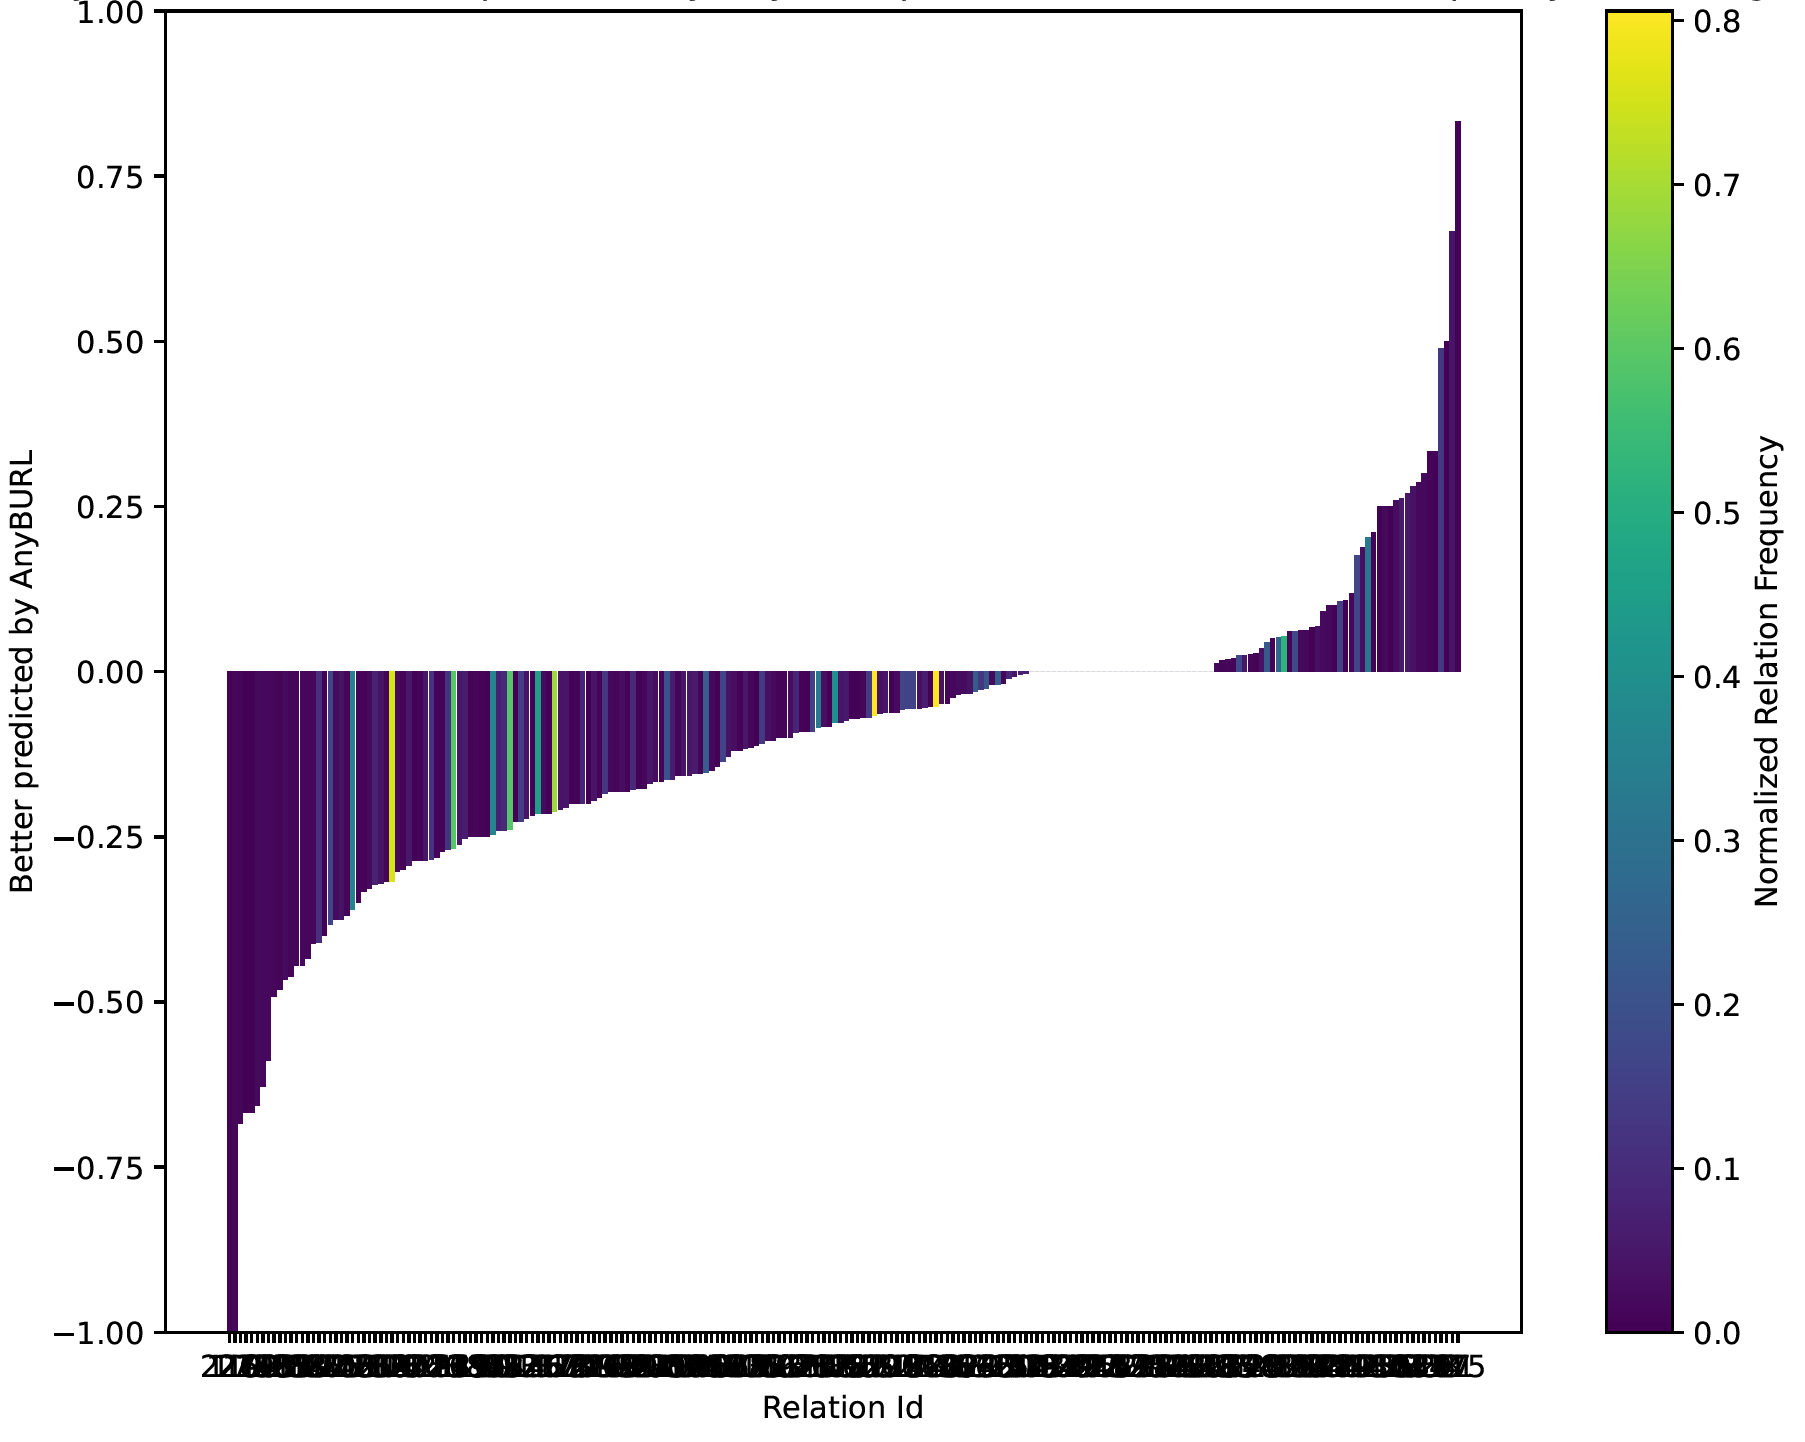
\includegraphics[width=0.7\textwidth]{images/relation_freq_anyburl_conve_fb15k.PNG}
\caption{Comparison of AnyBURL and ConvE on FB15k-237 in regard to the relation frequency}
\label{fig:relation_freq_anyburl_conve_fb15k}
\end{figure}

\begin{figure}[H]
\centering
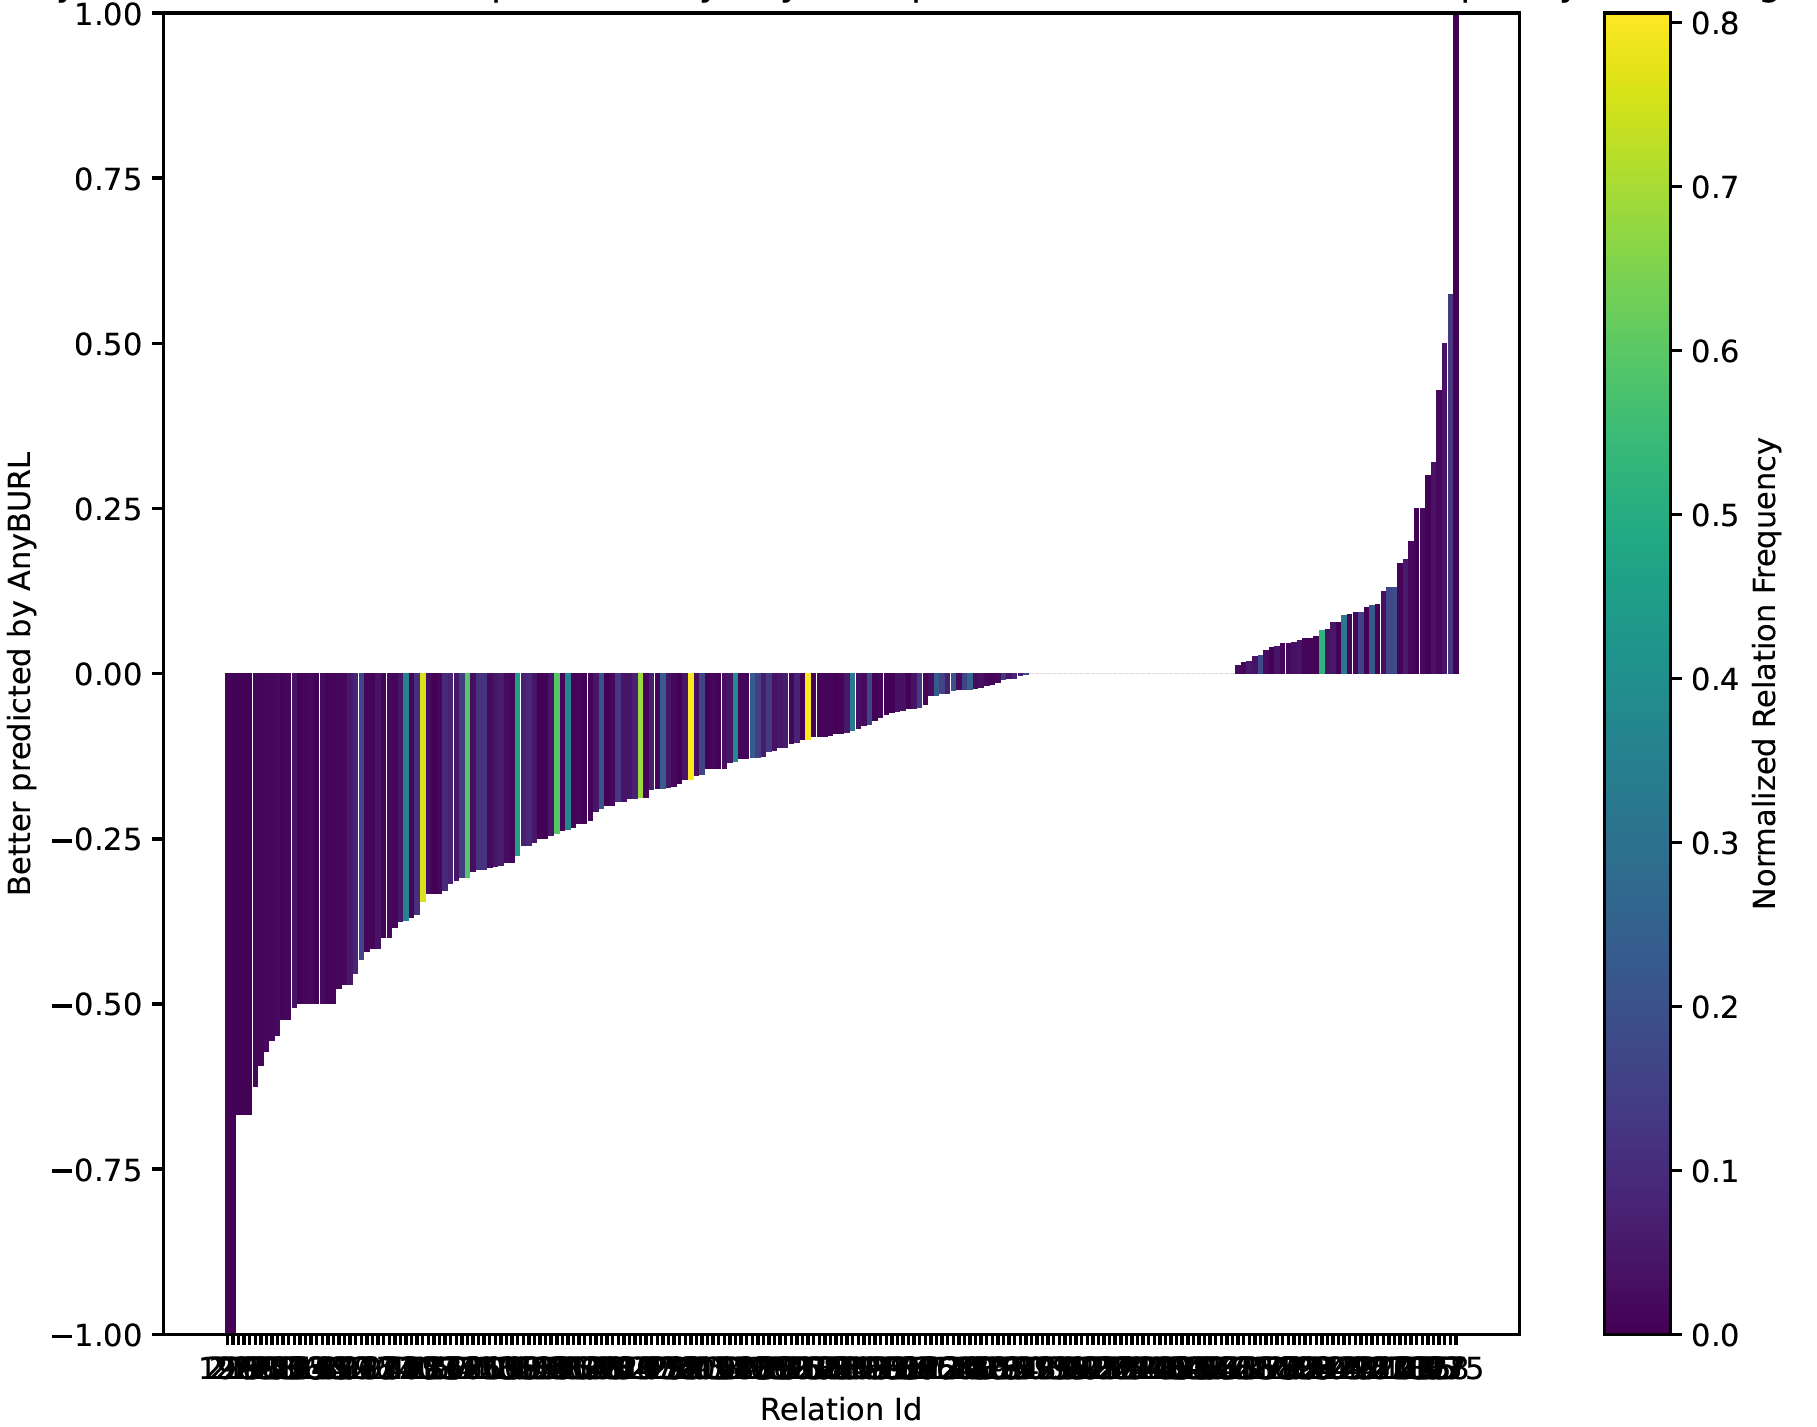
\includegraphics[width=0.7\textwidth]{images/relation_freq_anyburl_rescal_fb15k.PNG}
\caption{Comparison of AnyBURL and ConvE on FB15k-237 in regard to the relation frequency}
\label{fig:relation_freq_anyburl_rescal_fb15k}
\end{figure}
\section{Entity Frequency in Trainings Data}
\label{appendix:entity_freq}

\begin{figure}[H]
\centering
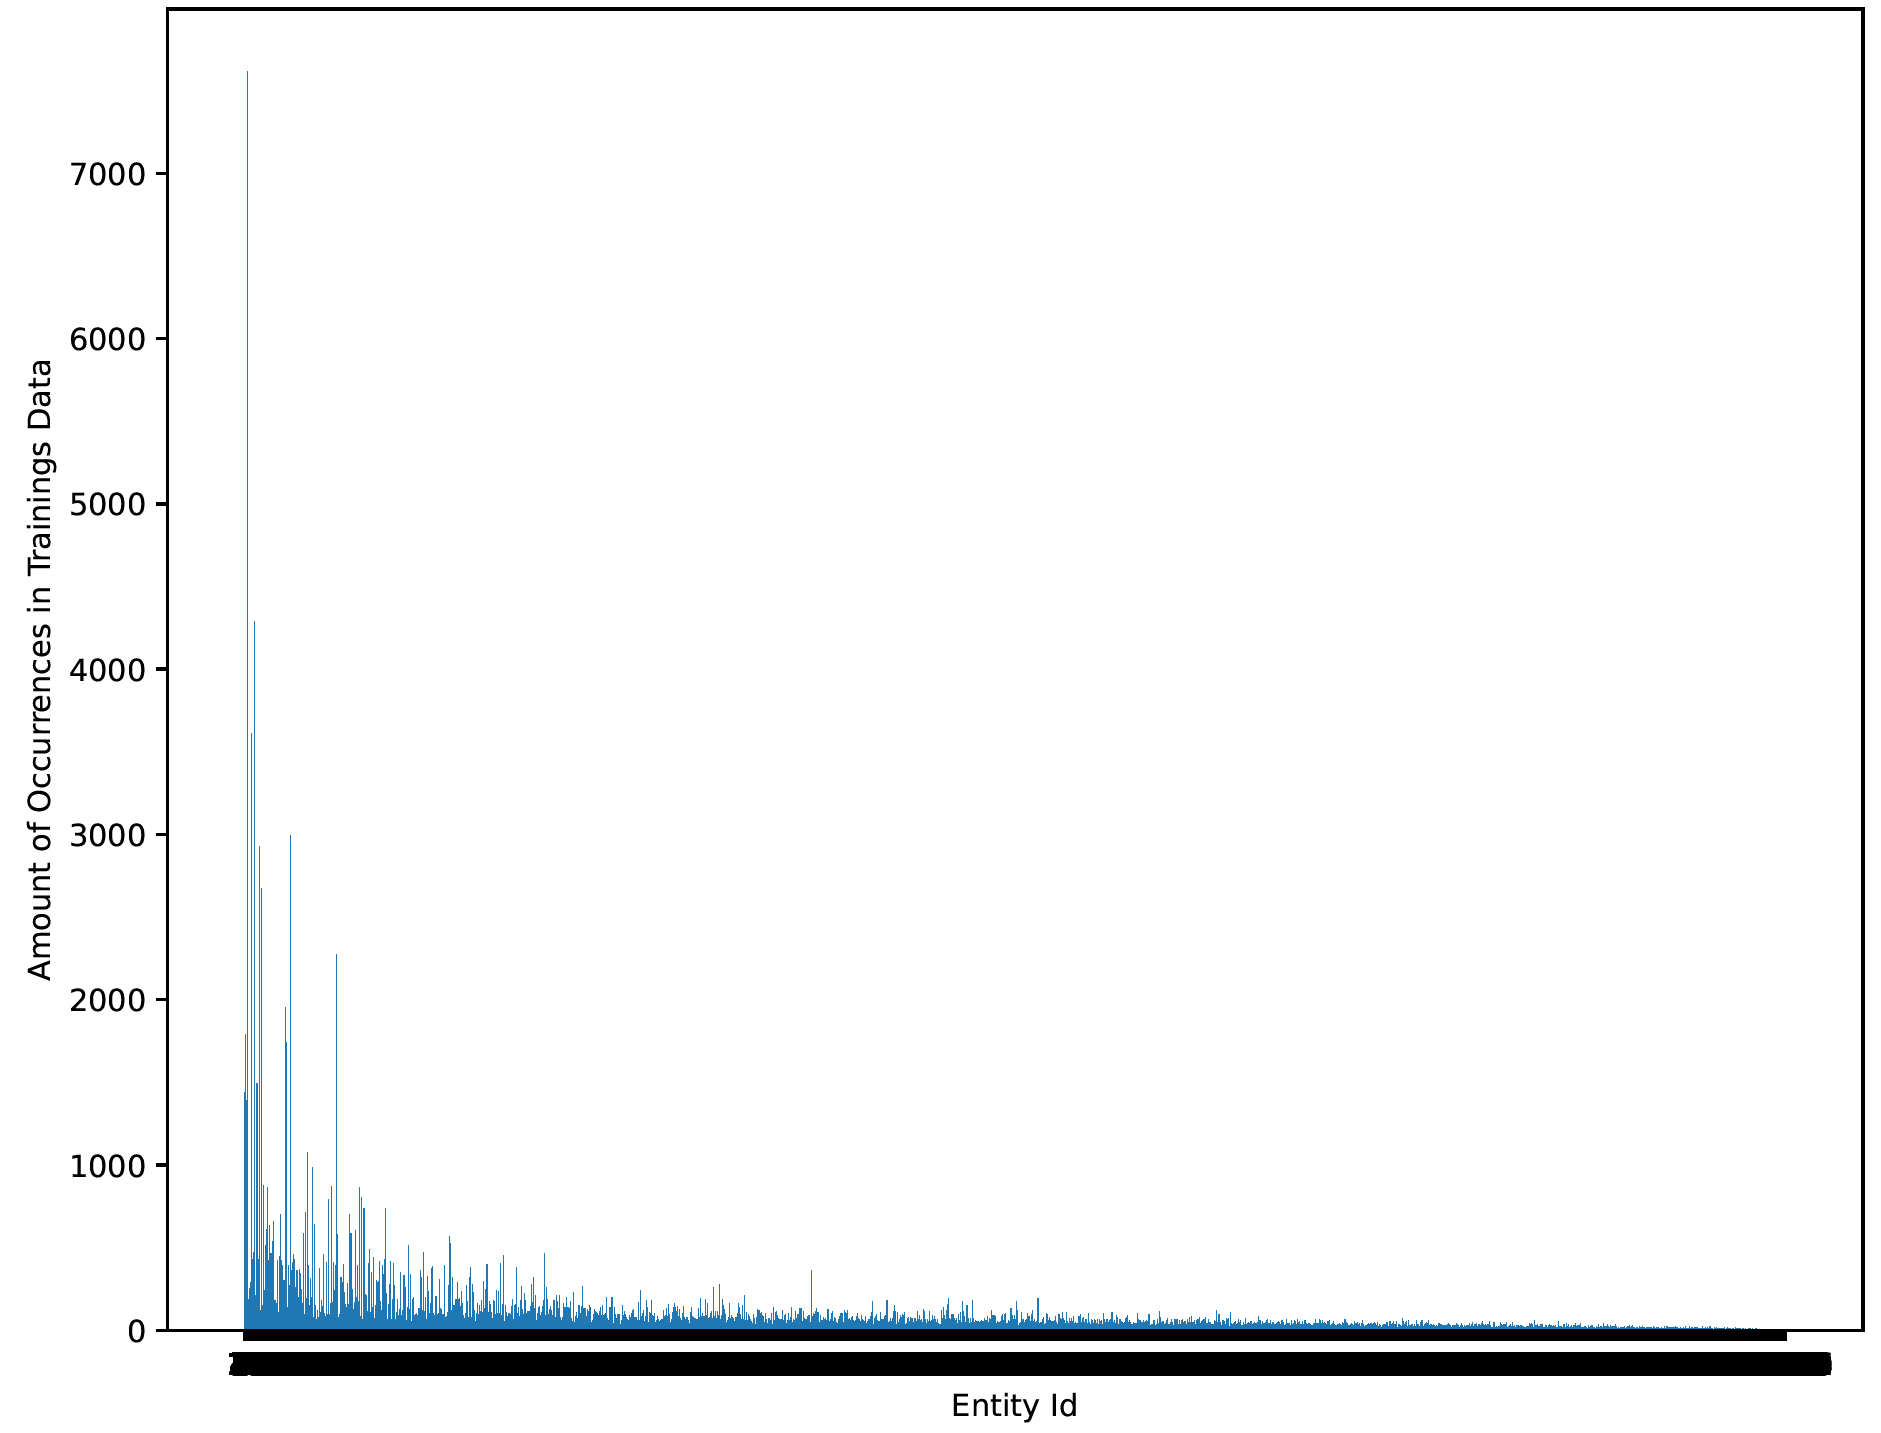
\includegraphics[width=0.7\textwidth]{images/entity_freq_fb15k.PNG}
\caption{Entity frequency in trainings data for FB15k-237}
\label{fig:entity_freq_fb15k}
\end{figure}

\begin{figure}[H]
\centering
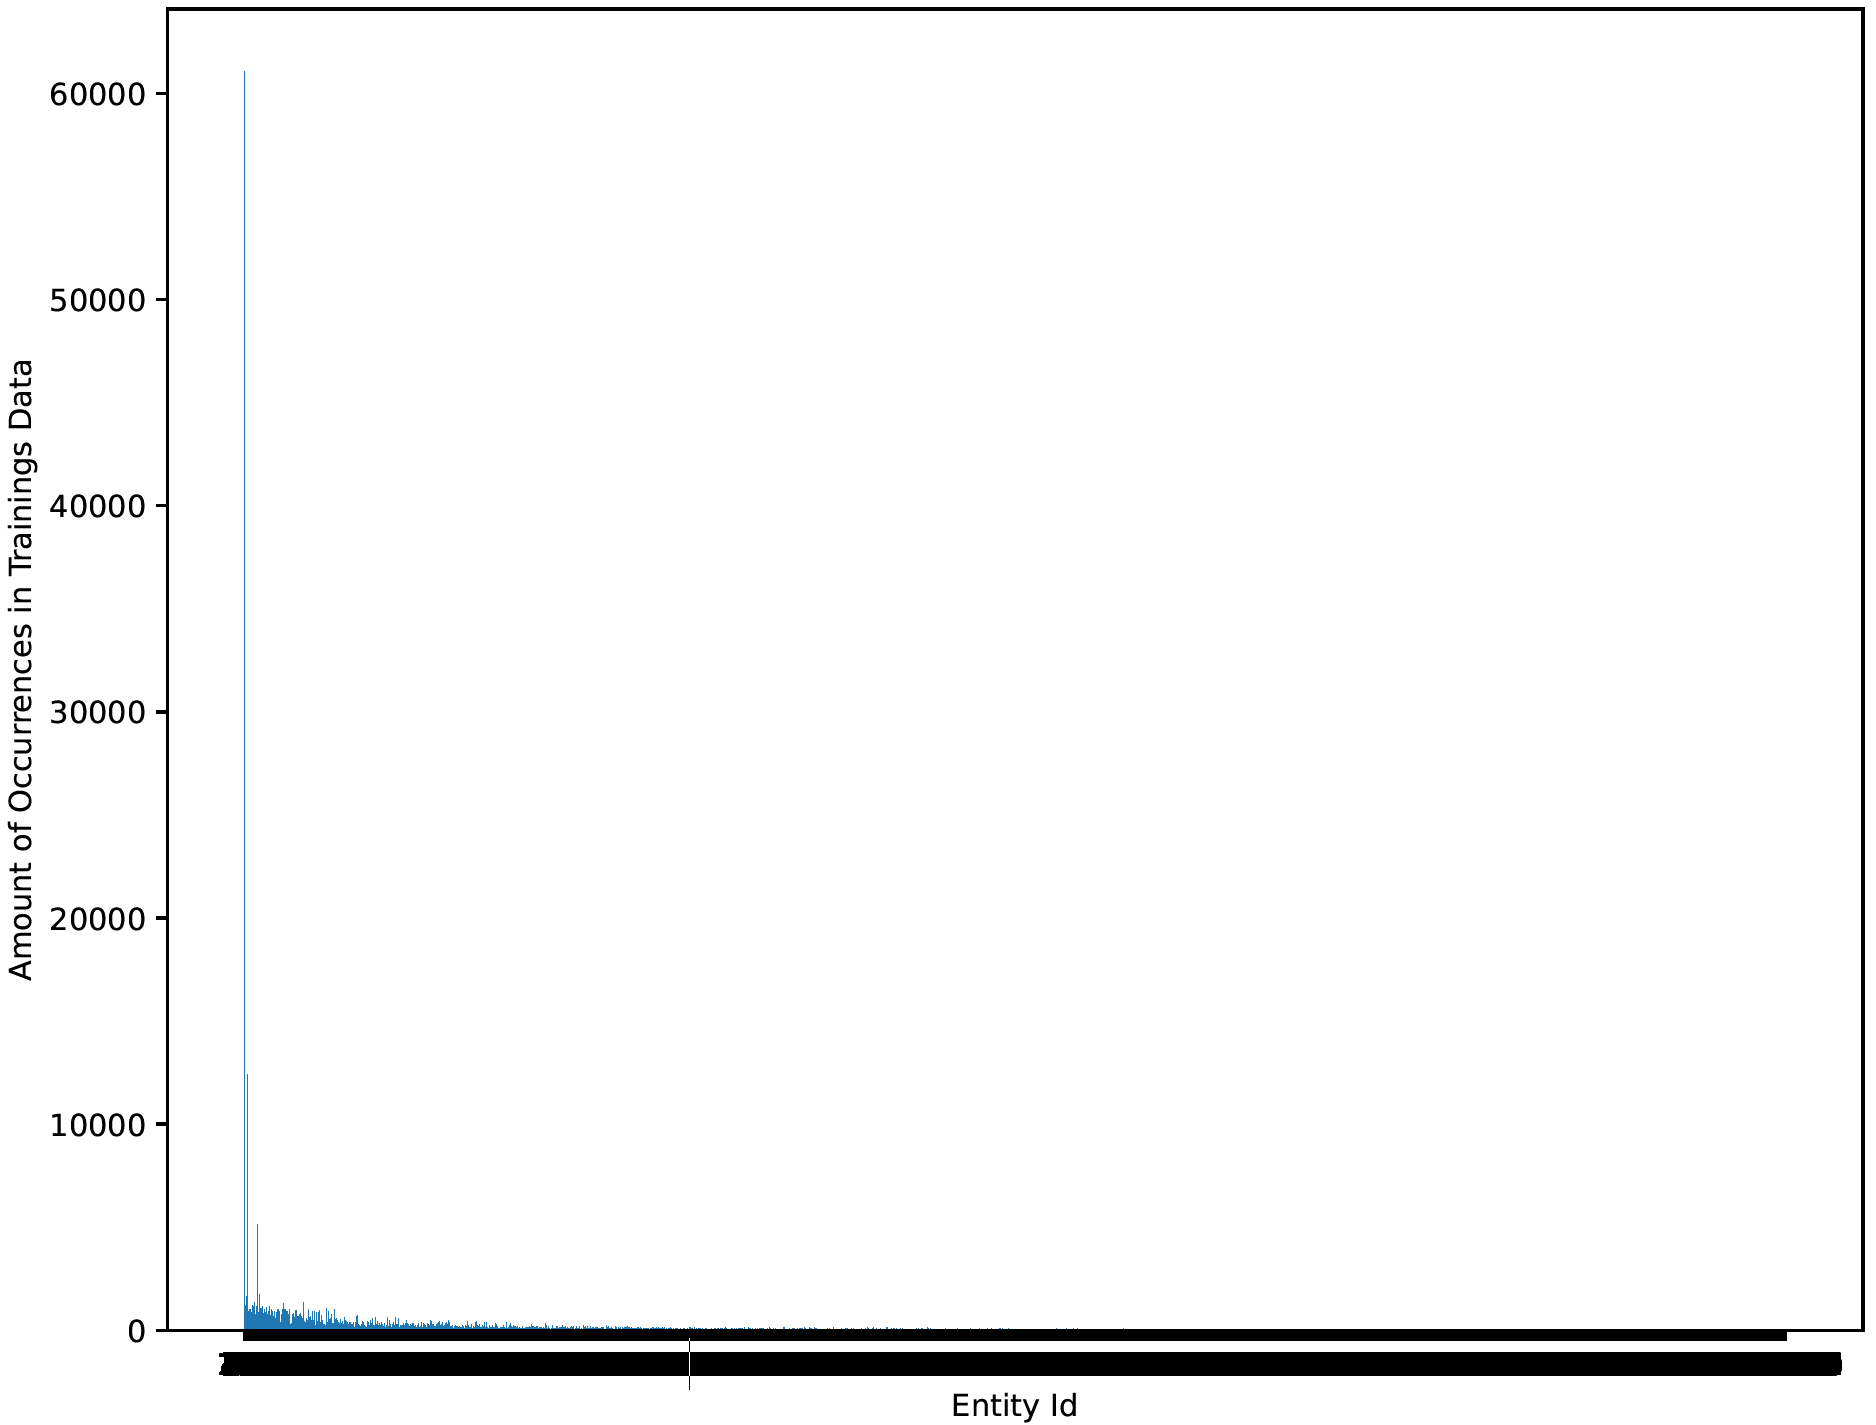
\includegraphics[width=0.7\textwidth]{images/entity_freq_yago.PNG}
\caption{Entity frequency in trainings data for YAGO3-10}
\label{fig:entity_freq_yago}
\end{figure}
\section{Comparison in regard to the Entity Frequency}
\label{appendix:comparison_entity_freq}

\subsection{AnyBURL and ConvE on CoDEx-M}

\begin{figure}[H]
\centering
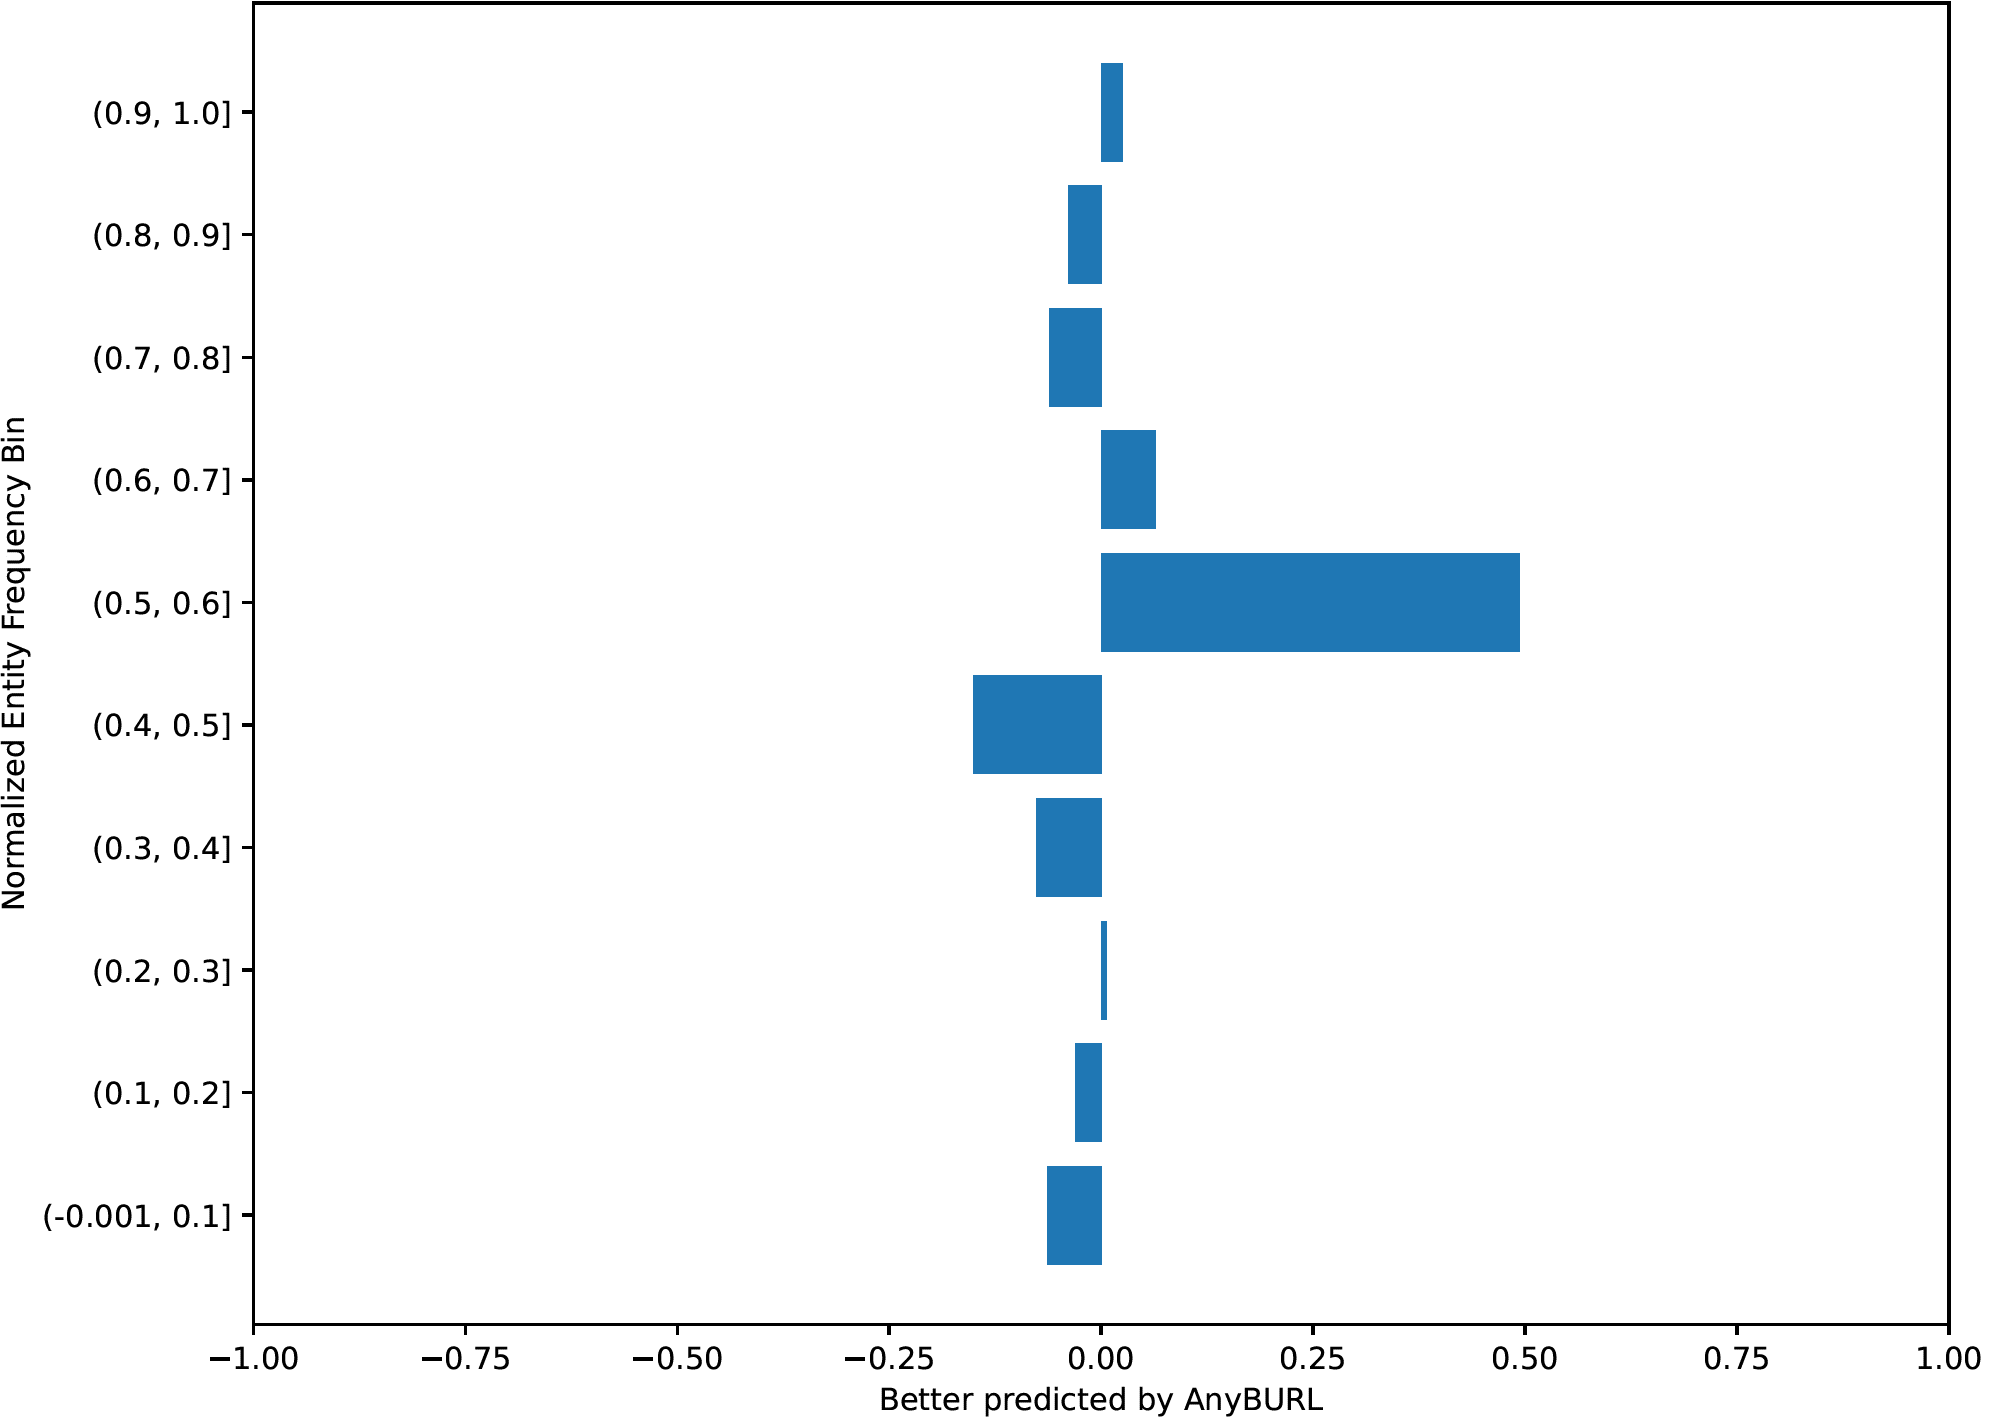
\includegraphics[width=0.7\textwidth]{images/entity_freq_question_anyburl_conve_codex.PNG}
\caption{Comparison of AnyBURL and ConvE on CodEx-M in regard to the question entity frequency}
\label{fig:entity_question_tail_anyburl_conve_codex}
\end{figure}

\begin{figure}[H]
\centering
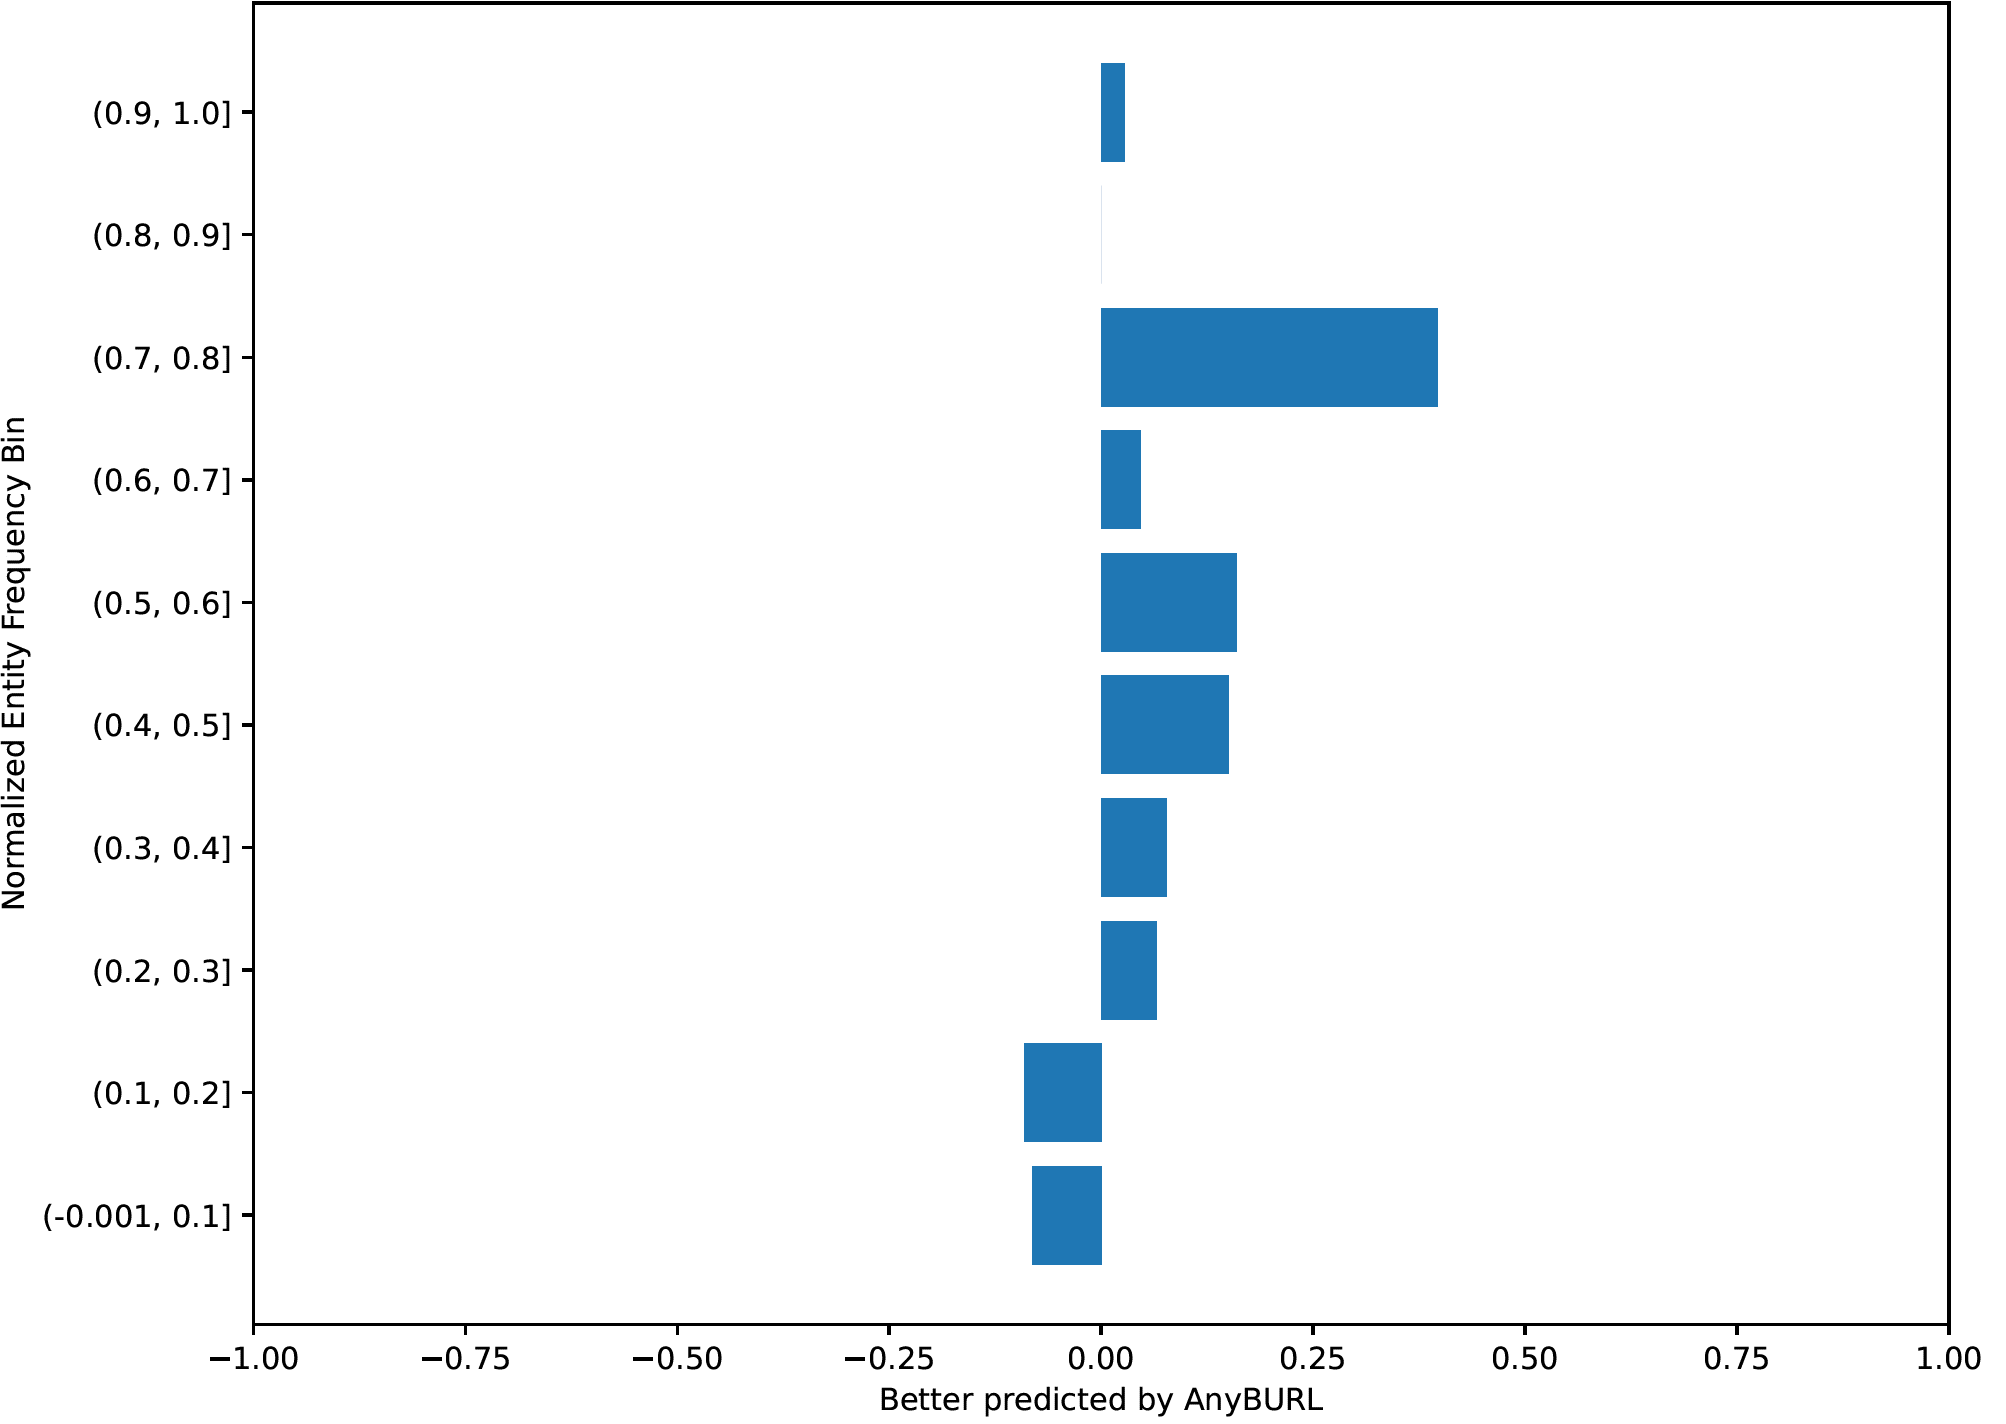
\includegraphics[width=0.7\textwidth]{images/entity_freq_answer_anyburl_conve_codex.PNG}
\caption{Comparison of AnyBURL and ConvE on CodEx-M in regard to the answer entity frequency}
\label{fig:entity_answer_tail_anyburl_conve_codex}
\end{figure}

\begin{figure}[H]
\centering
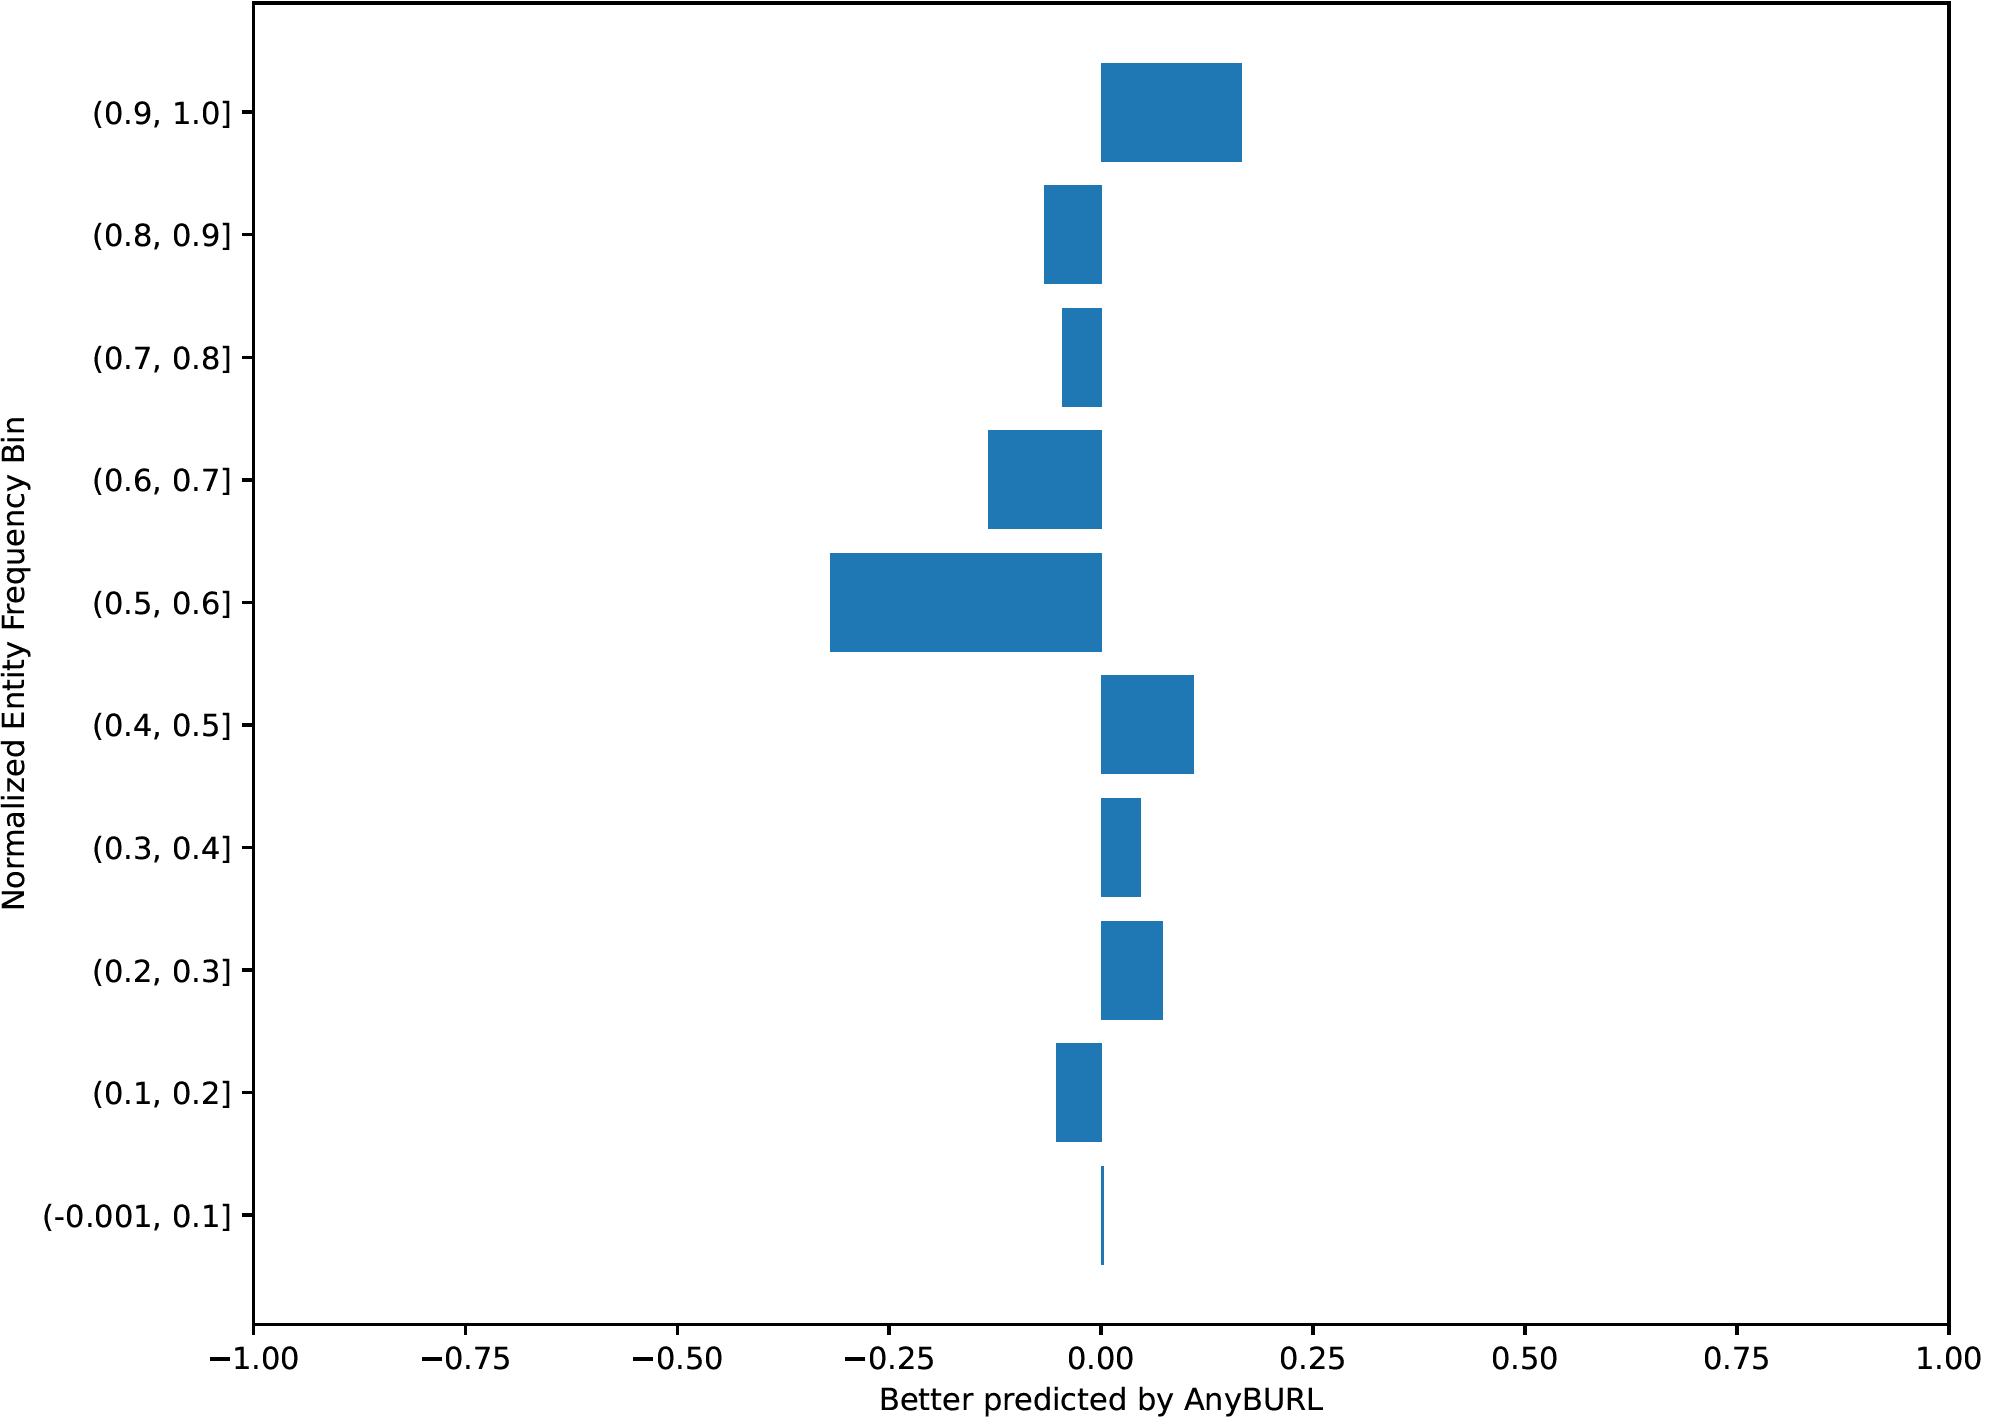
\includegraphics[width=0.7\textwidth]{images/combined_freq_anyburl_conve_codex.PNG}
\caption{Comparison of AnyBURL and ConvE on CodEx-M in regard to the combined entity and relation frequency}
\label{fig:combined_freq_anyburl_conve_codex}
\end{figure}



\subsection{AnyBURL and RESCAL on CoDEx-M}

\begin{figure}[H]
\centering
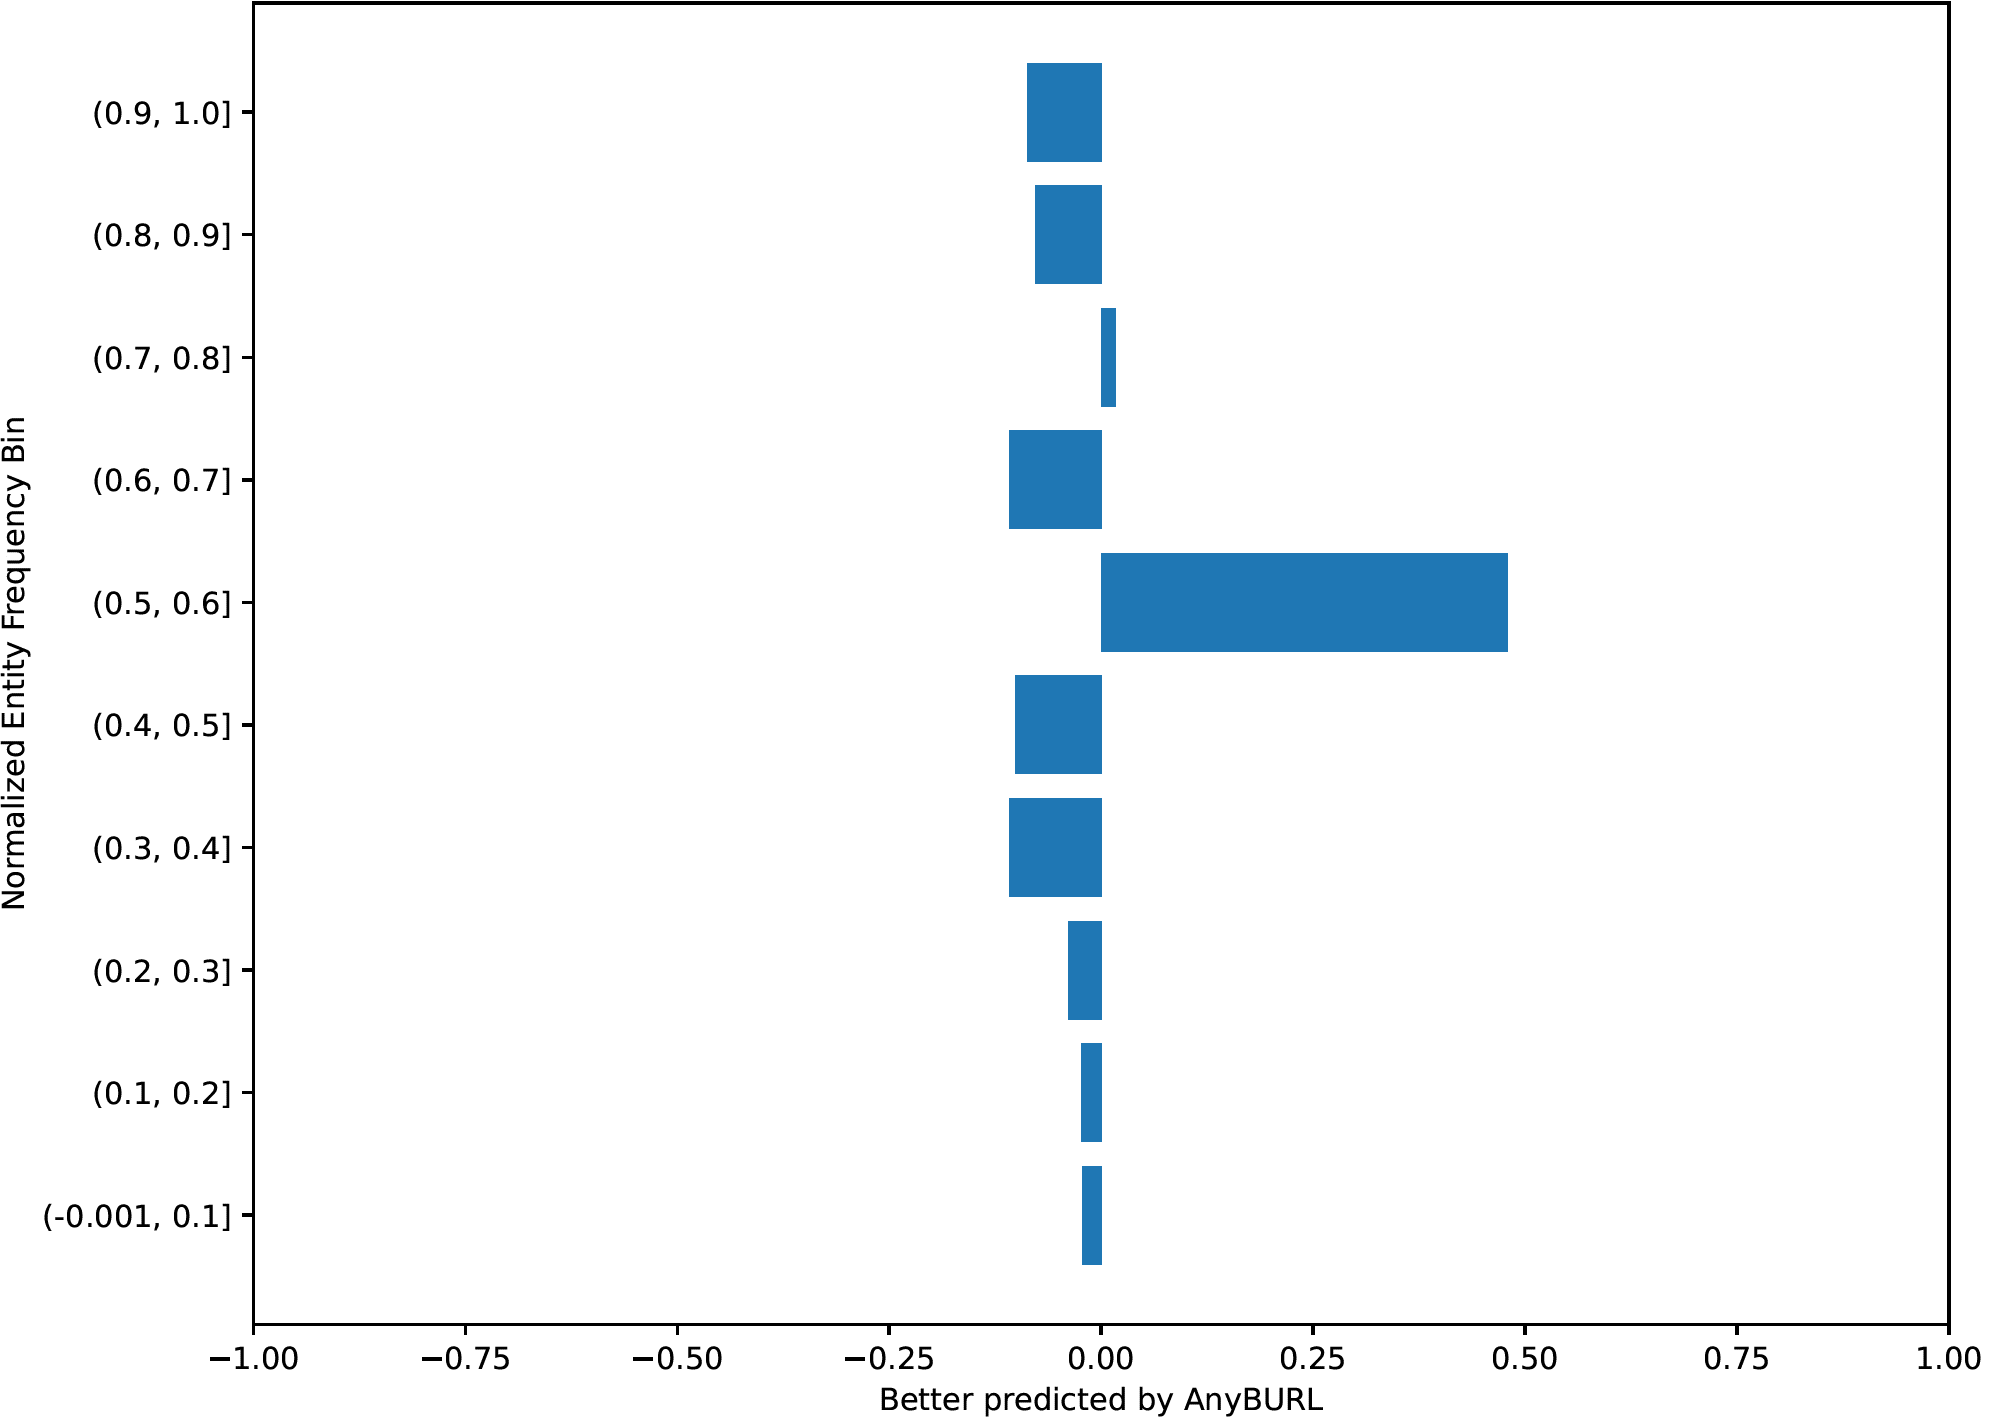
\includegraphics[width=0.7\textwidth]{images/entity_freq_question_anyburl_rescal_codex.PNG}
\caption{Comparison of AnyBURL and RESCAL on CodEx-M in regard to the question entity frequency}
\label{fig:entity_question_tail_anyburl_rescal_codex}
\end{figure}

\begin{figure}[H]
\centering
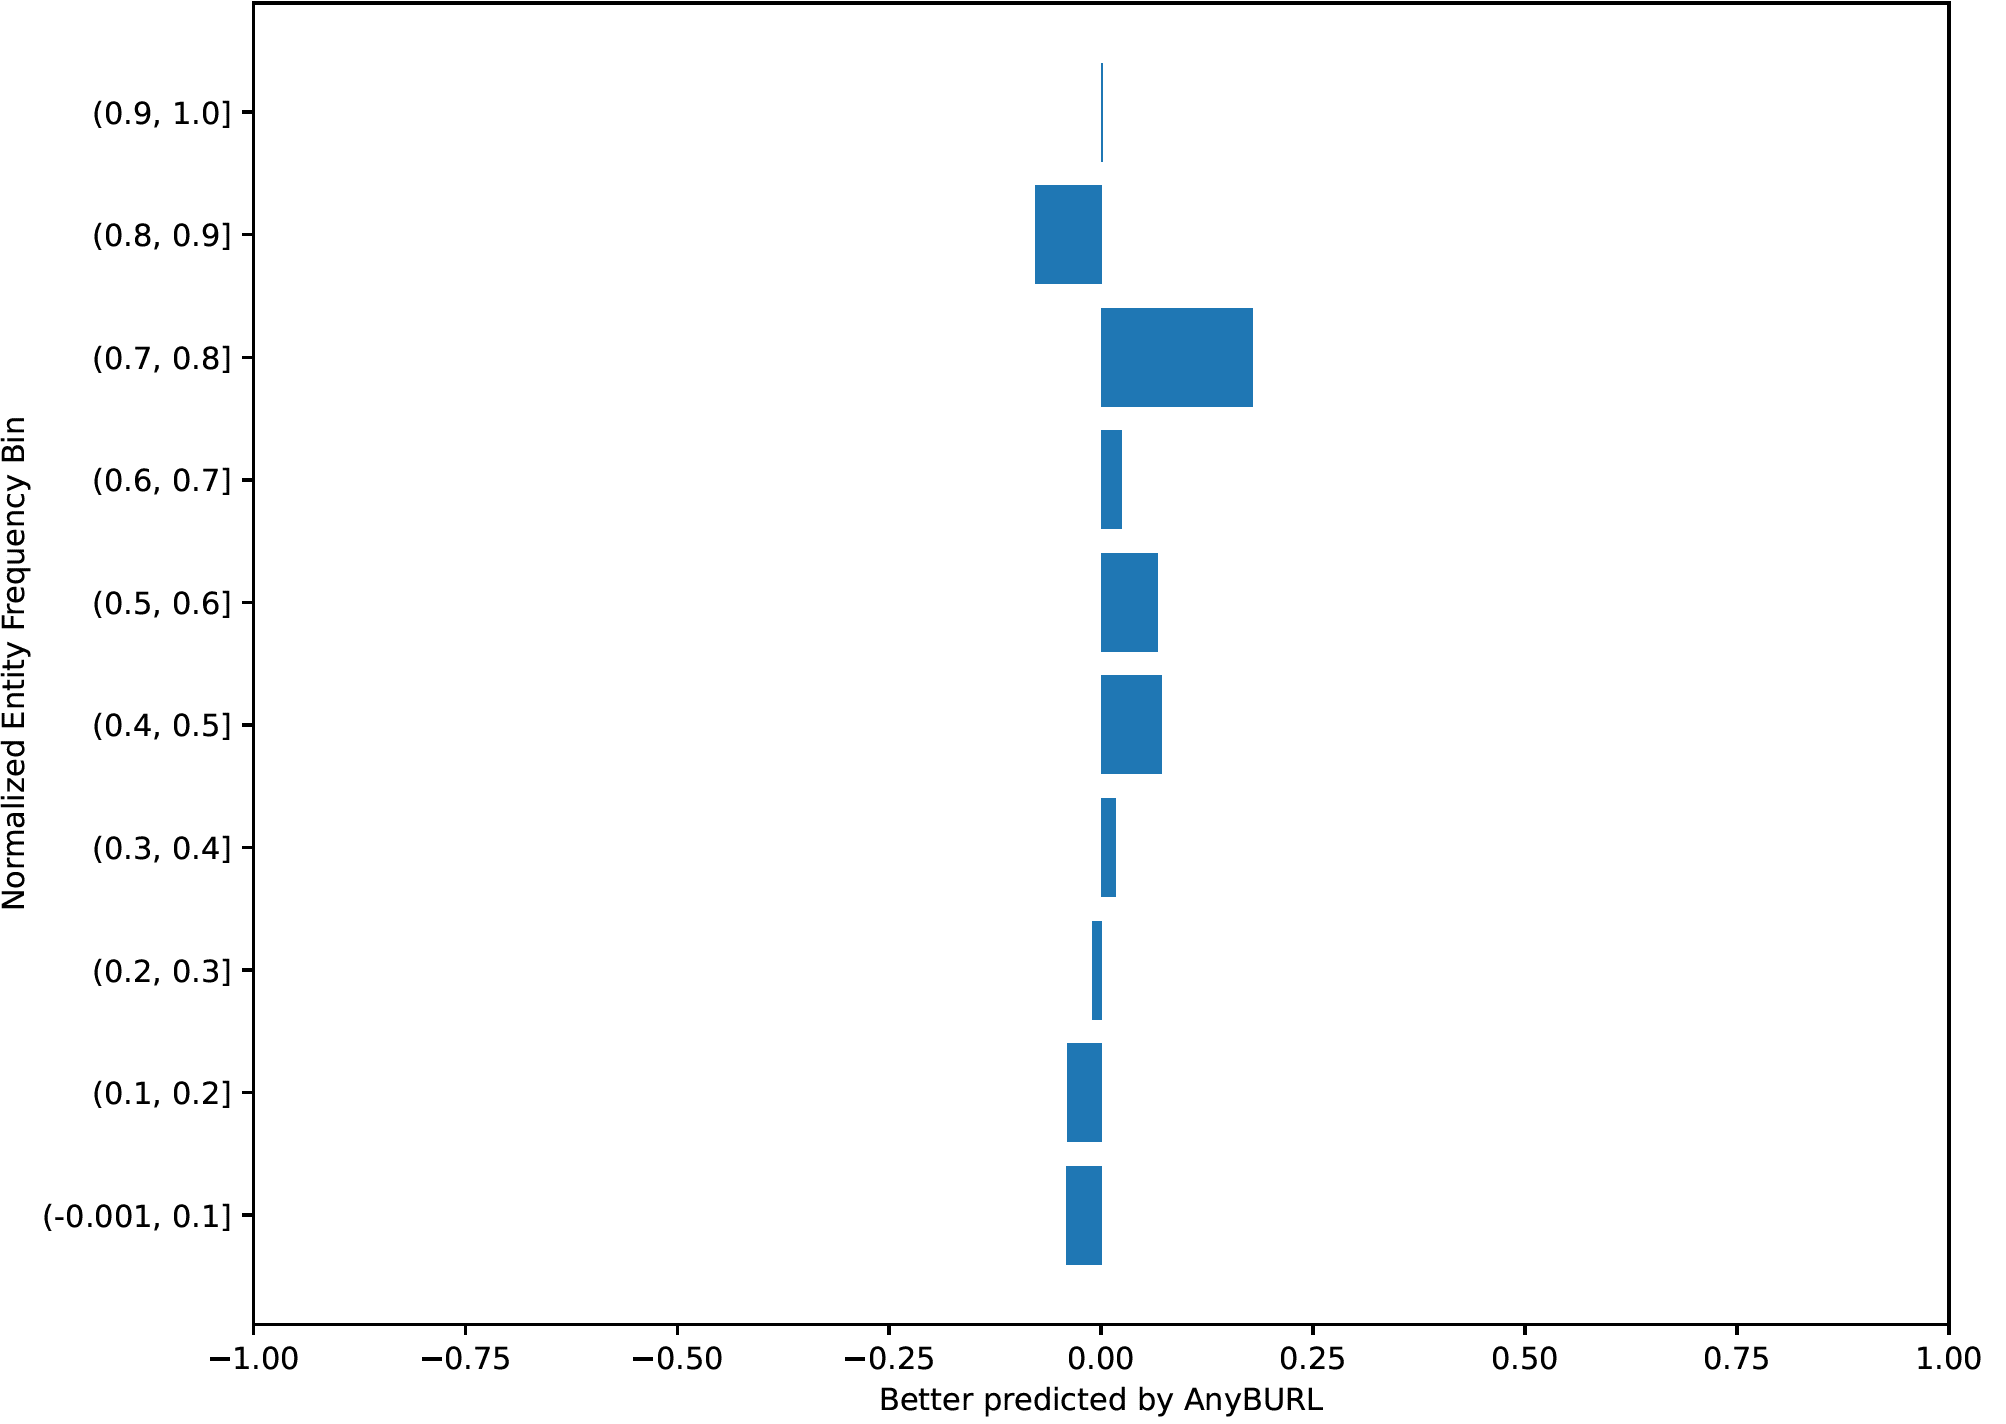
\includegraphics[width=0.7\textwidth]{images/entity_freq_answer_anyburl_rescal_codex.PNG}
\caption{Comparison of AnyBURL and RESCAL on CodEx-M in regard to the answer entity frequency}
\label{fig:entity_answer_tail_anyburl_rescal_codex}
\end{figure}

\begin{figure}[H]
\centering
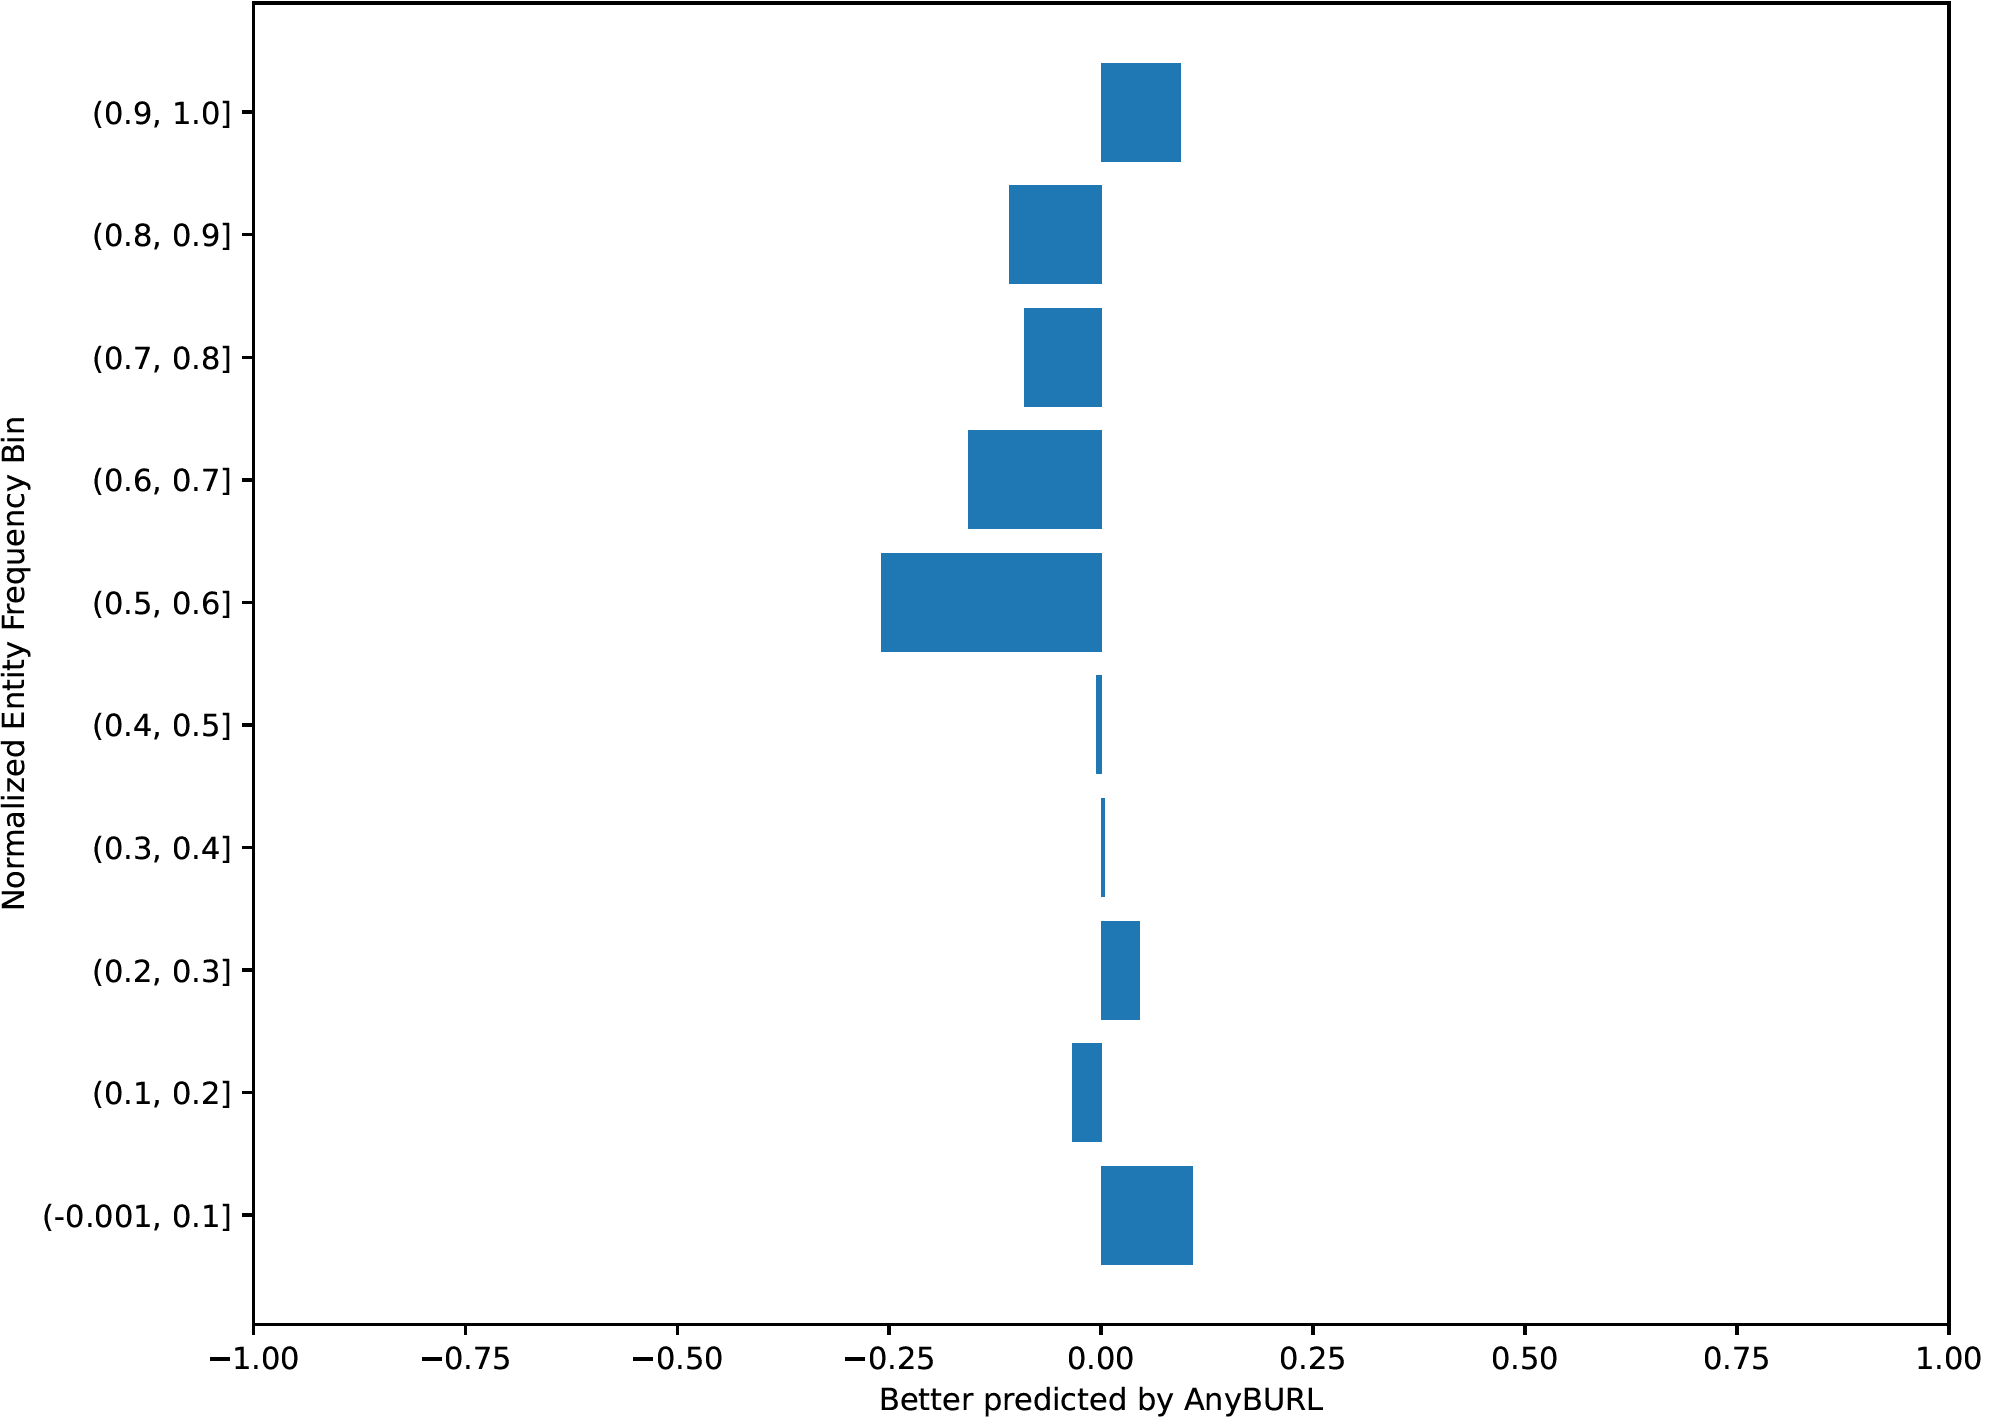
\includegraphics[width=0.7\textwidth]{images/combined_freq_anyburl_rescal_codex.PNG}
\caption{Comparison of AnyBURL and RESCAL on CodEx-M in regard to the combined entity and relation frequency}
\label{fig:combined_freq_anyburl_rescal_codex}
\end{figure}


\subsection{AnyBURL and ComplEx on FB15k-237}

\begin{figure}[H]
\centering
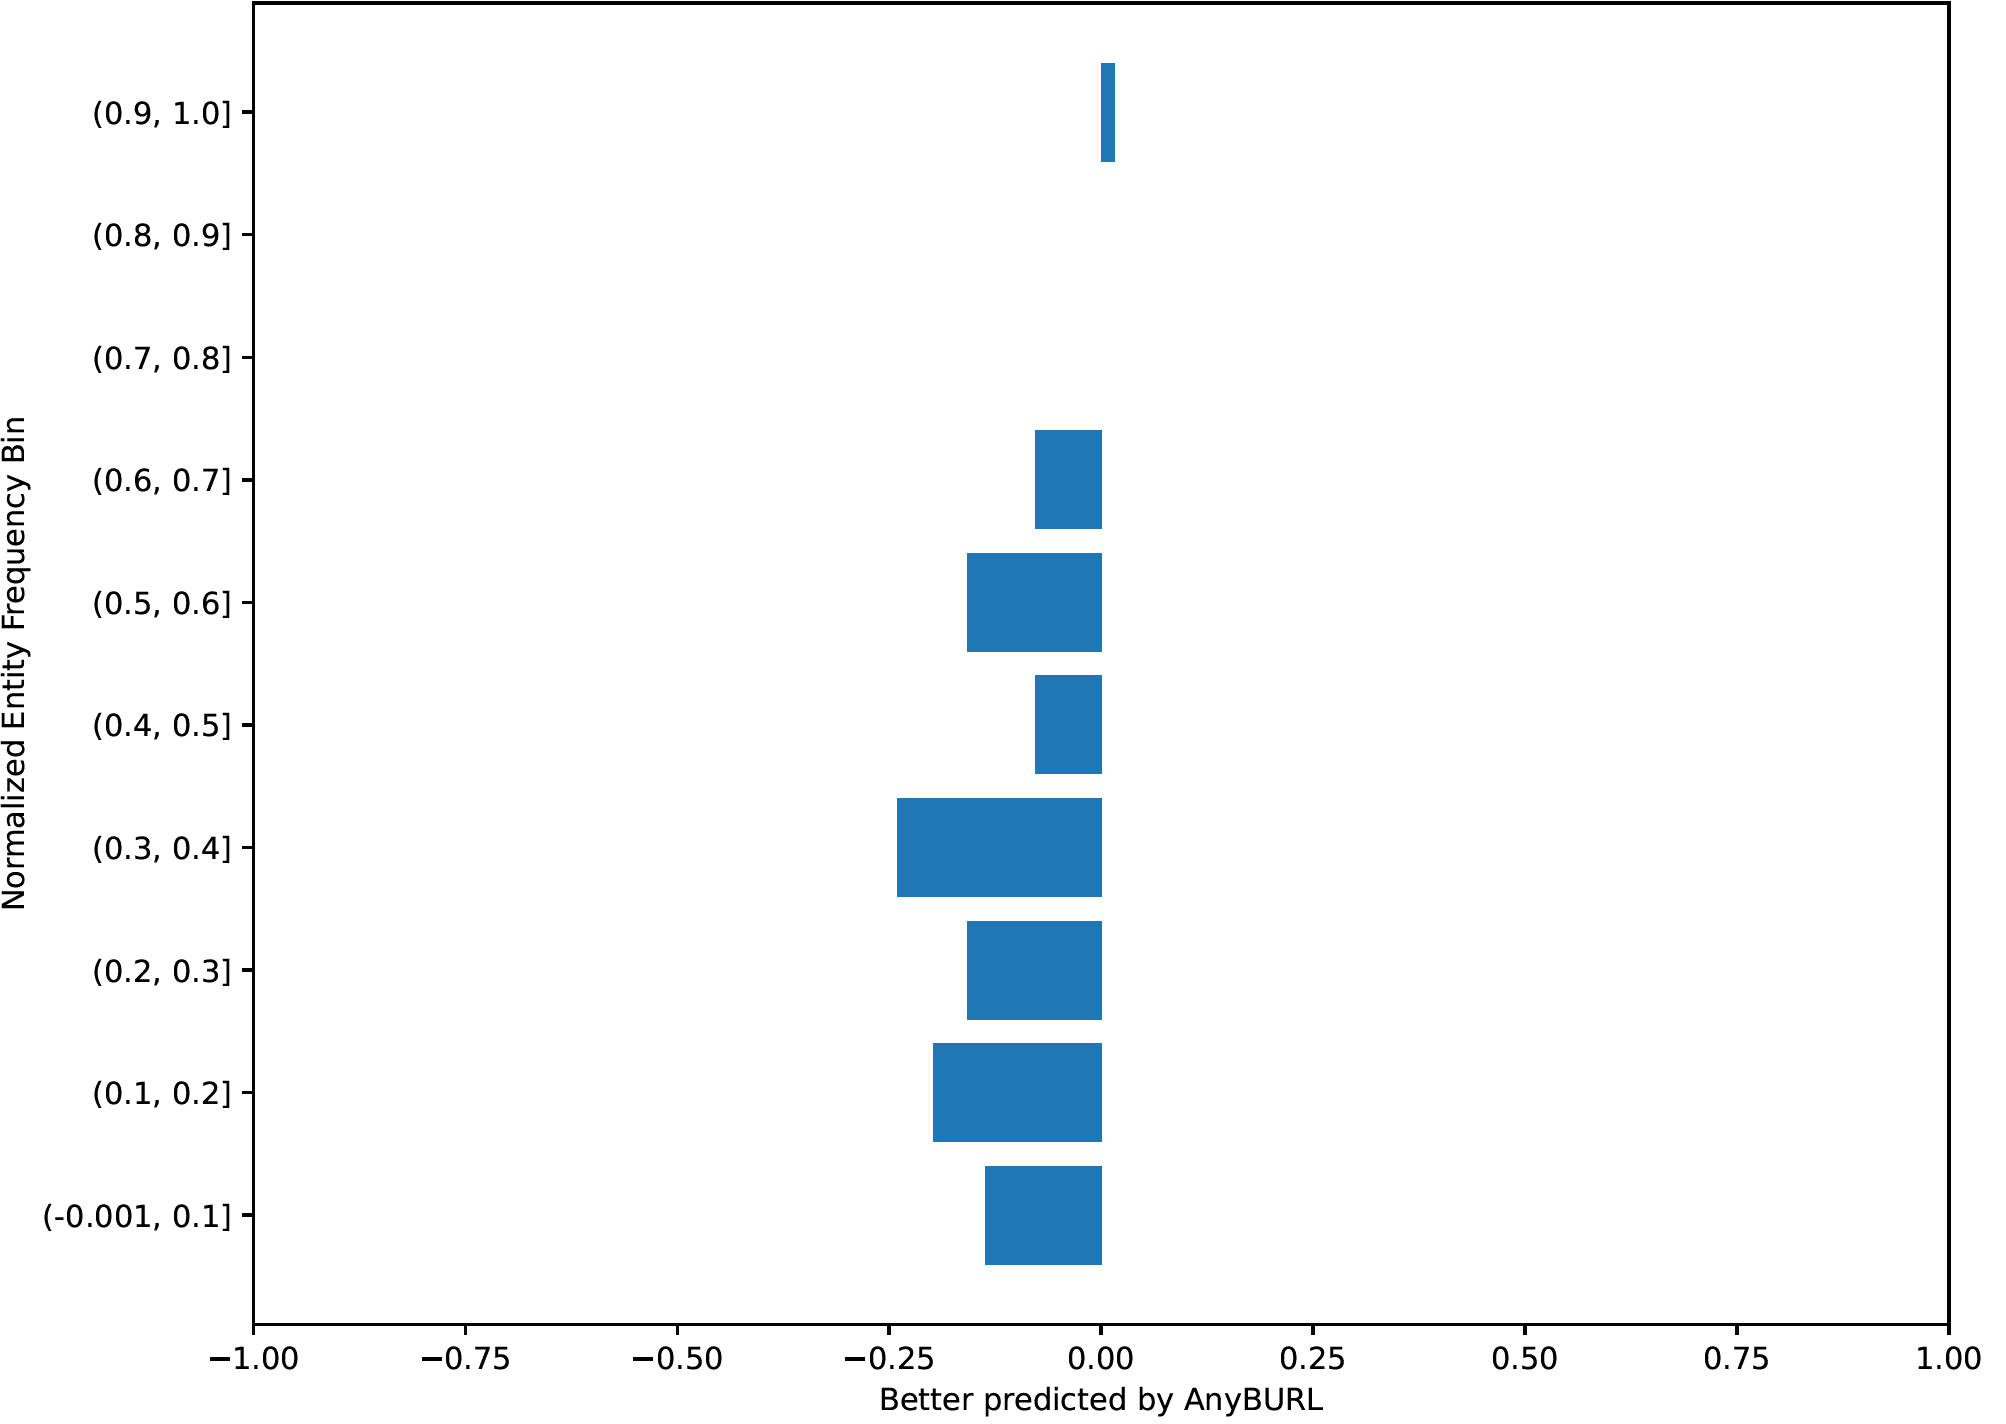
\includegraphics[width=0.7\textwidth]{images/entity_freq_question_anyburl_complex_fb15k.PNG}
\caption{Comparison of AnyBURL and ComplEx on FB15k-237 in regard to the question entity frequency}
\label{fig:entity_question_tail_anyburl_complex_fb15k}
\end{figure}

\begin{figure}[H]
\centering
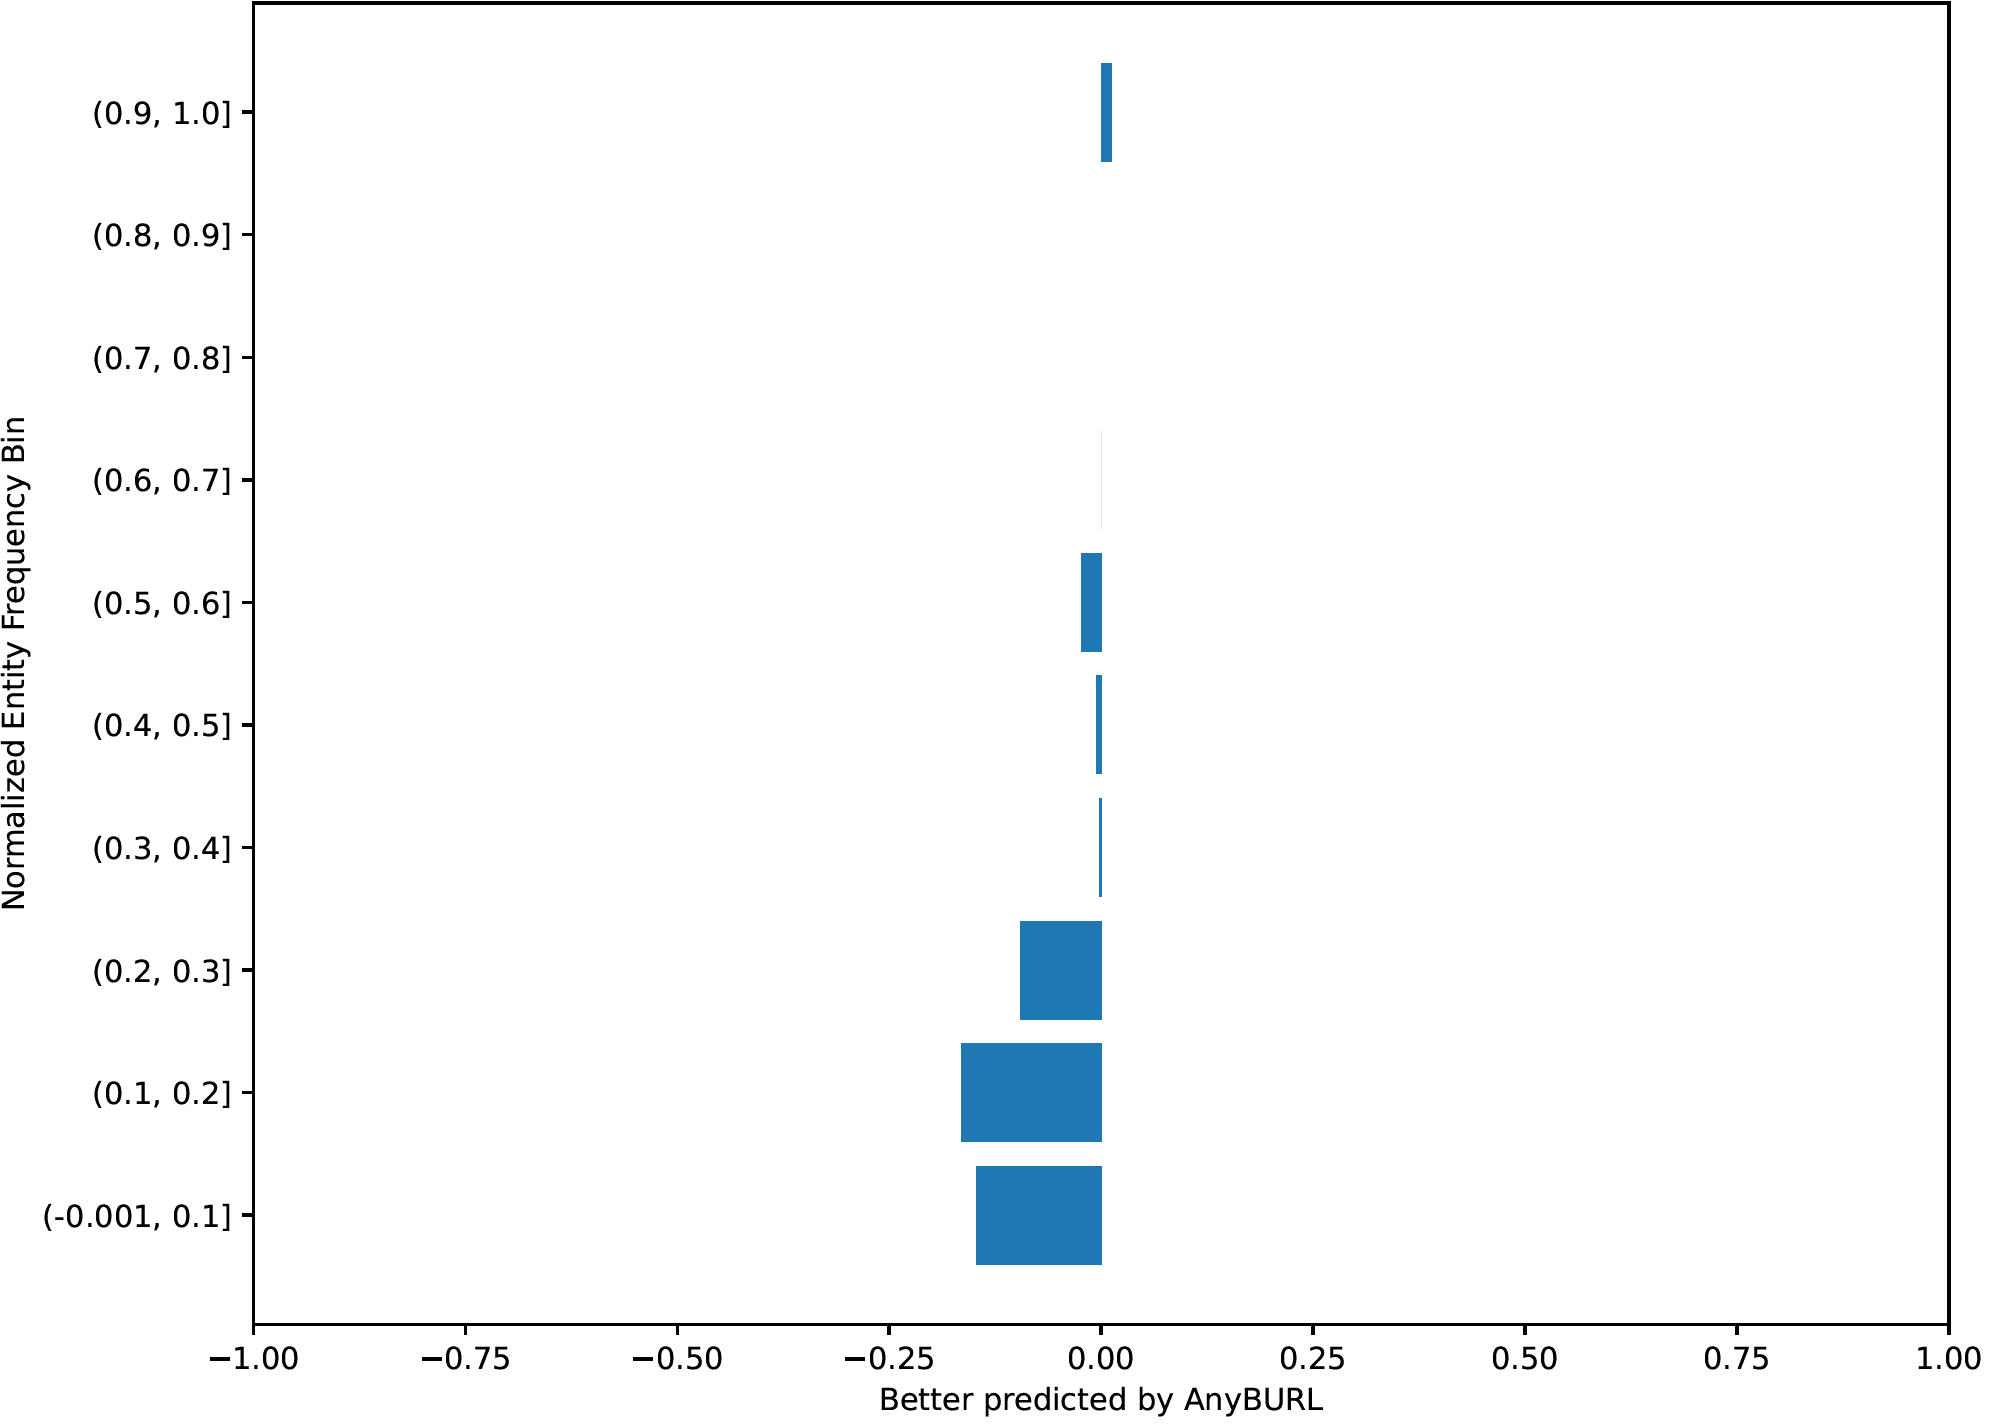
\includegraphics[width=0.7\textwidth]{images/entity_freq_answer_anyburl_complex_fb15k.PNG}
\caption{Comparison of AnyBURL and ComplEx on FB15k-237 in regard to the answer entity frequency}
\label{fig:entity_answer_tail_anyburl_complex_fb15k}
\end{figure}

\begin{figure}[H]
\centering
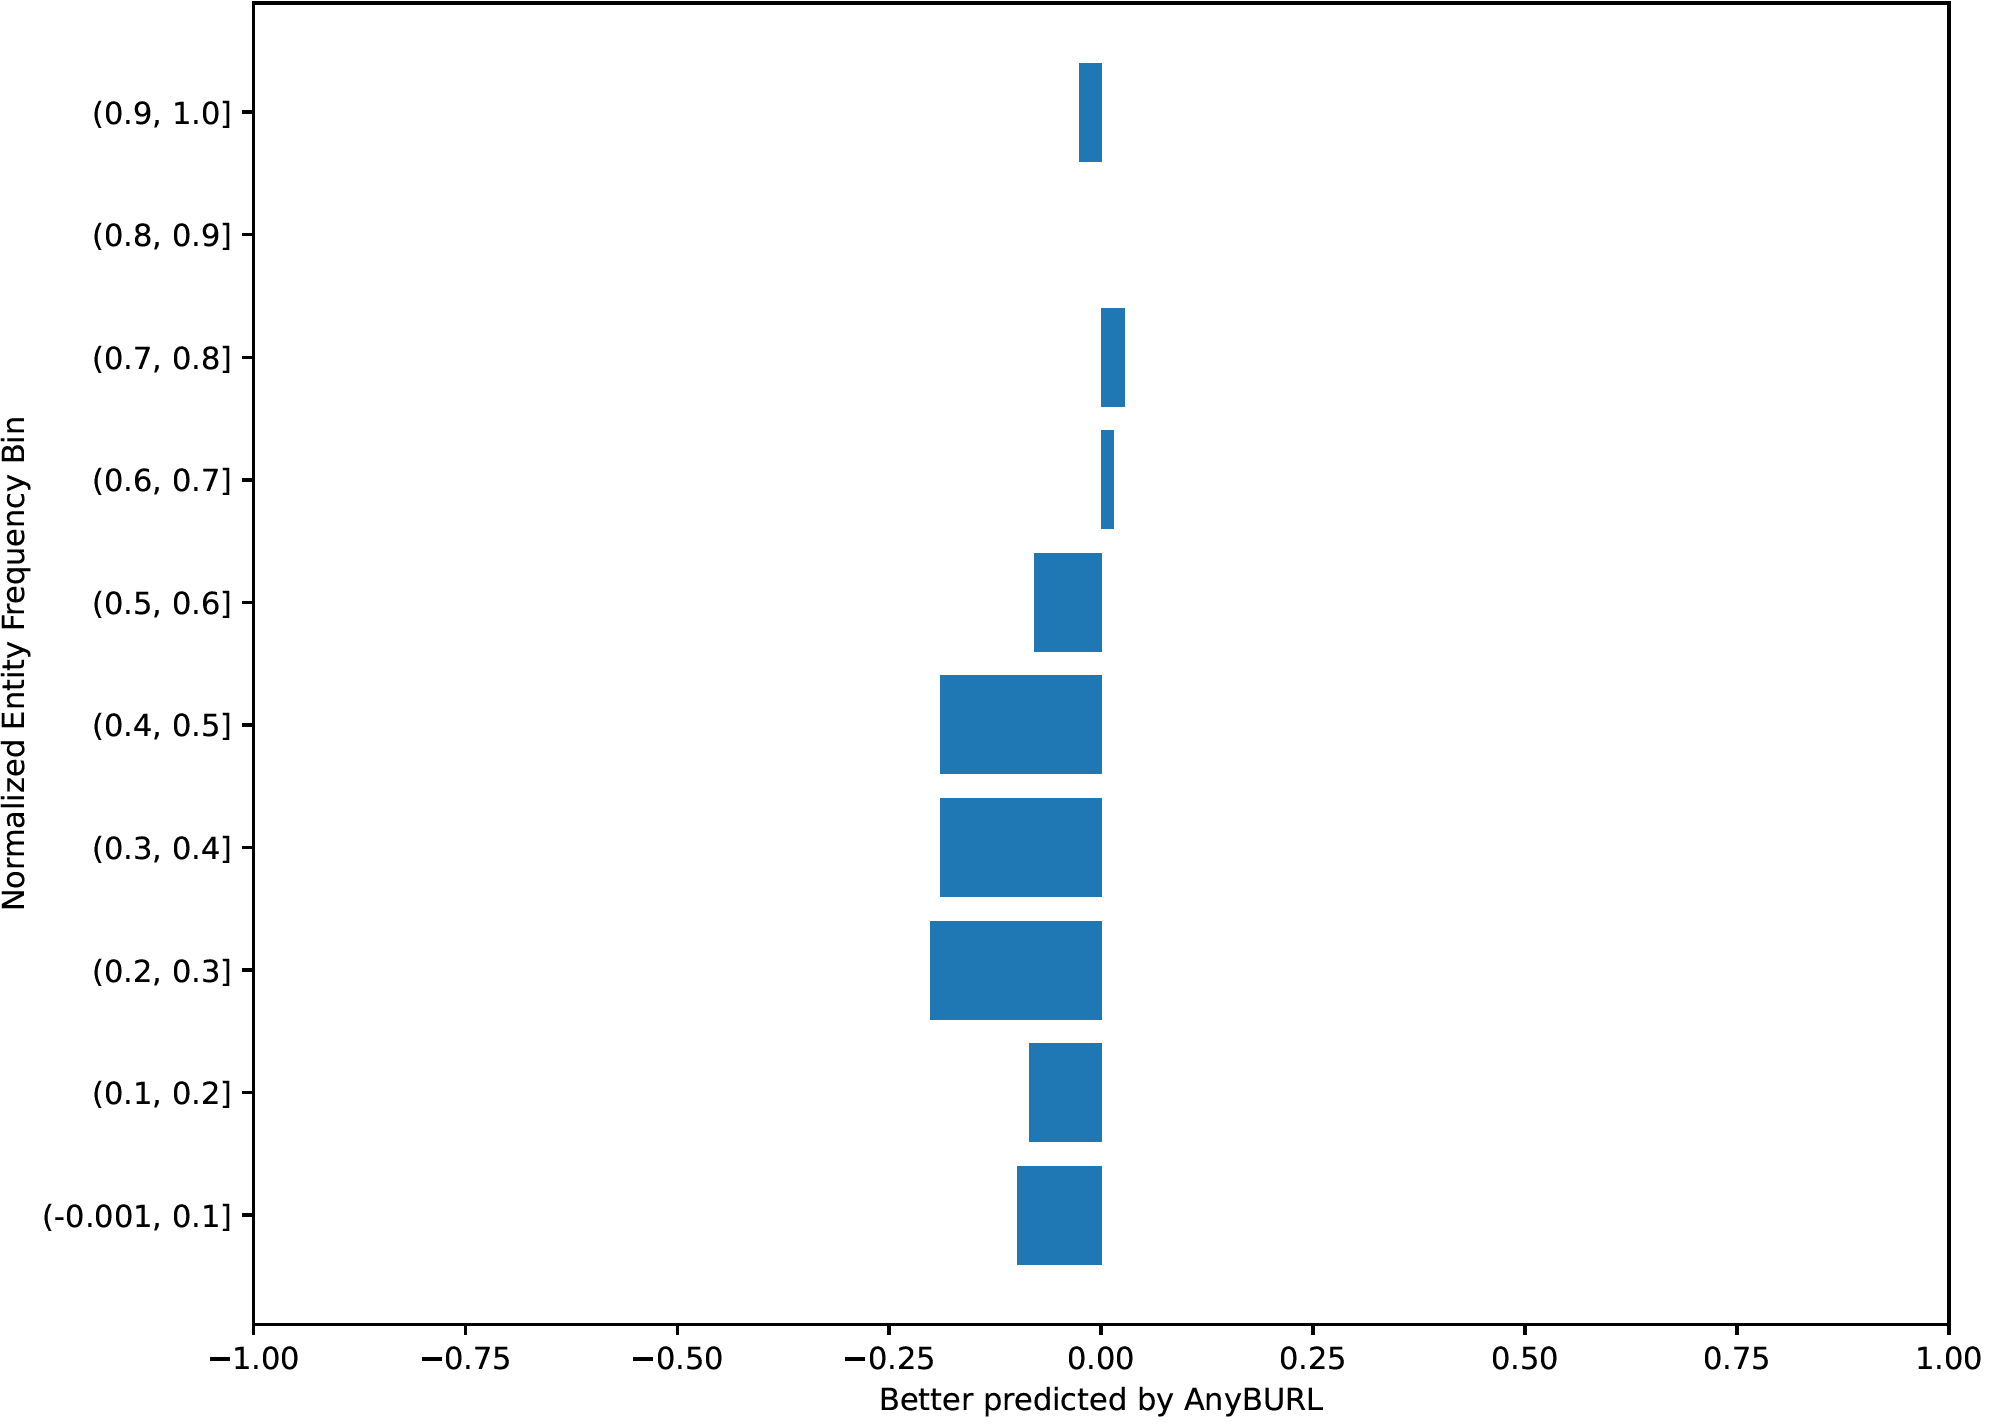
\includegraphics[width=0.7\textwidth]{images/combined_freq_anyburl_complex_fb15k.PNG}
\caption{Comparison of AnyBURL and ComplEx on FB15k-237 in regard to the combined entity and relation frequency}
\label{fig:combined_freq_anyburl_complex_fb15k}
\end{figure}





\subsection{AnyBURL and ConvE on FB15k-237}

\begin{figure}[H]
\centering
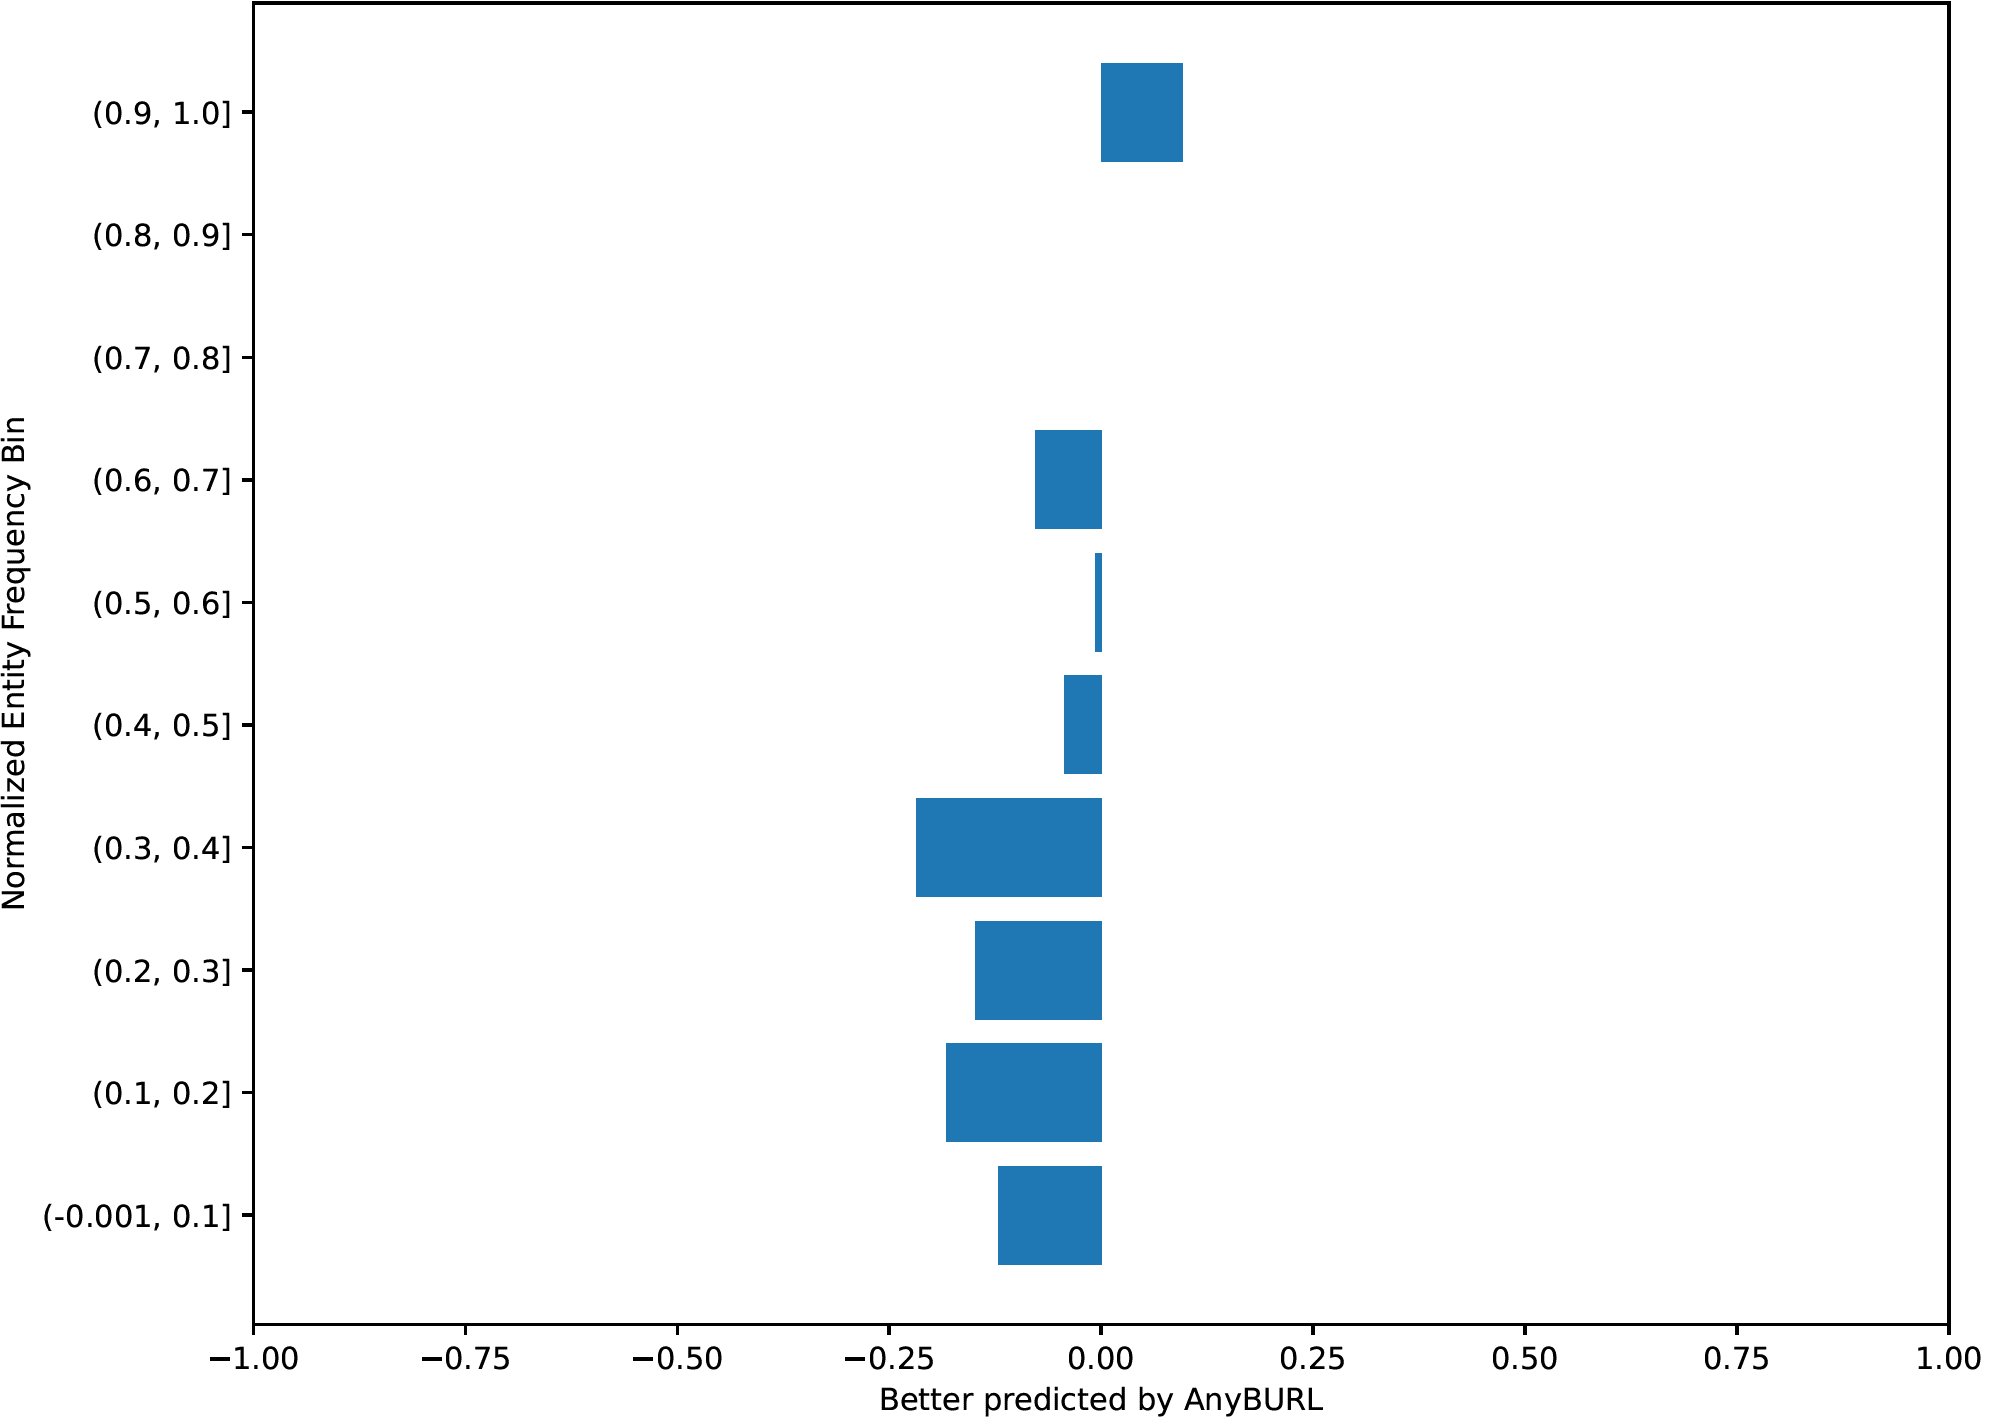
\includegraphics[width=0.7\textwidth]{images/entity_freq_question_anyburl_conve_fb15k.PNG}
\caption{Comparison of AnyBURL and ConvE on FB15k-237 in regard to the question entity frequency}
\label{fig:entity_question_tail_anyburl_conve_fb15k}
\end{figure}

\begin{figure}[H]
\centering
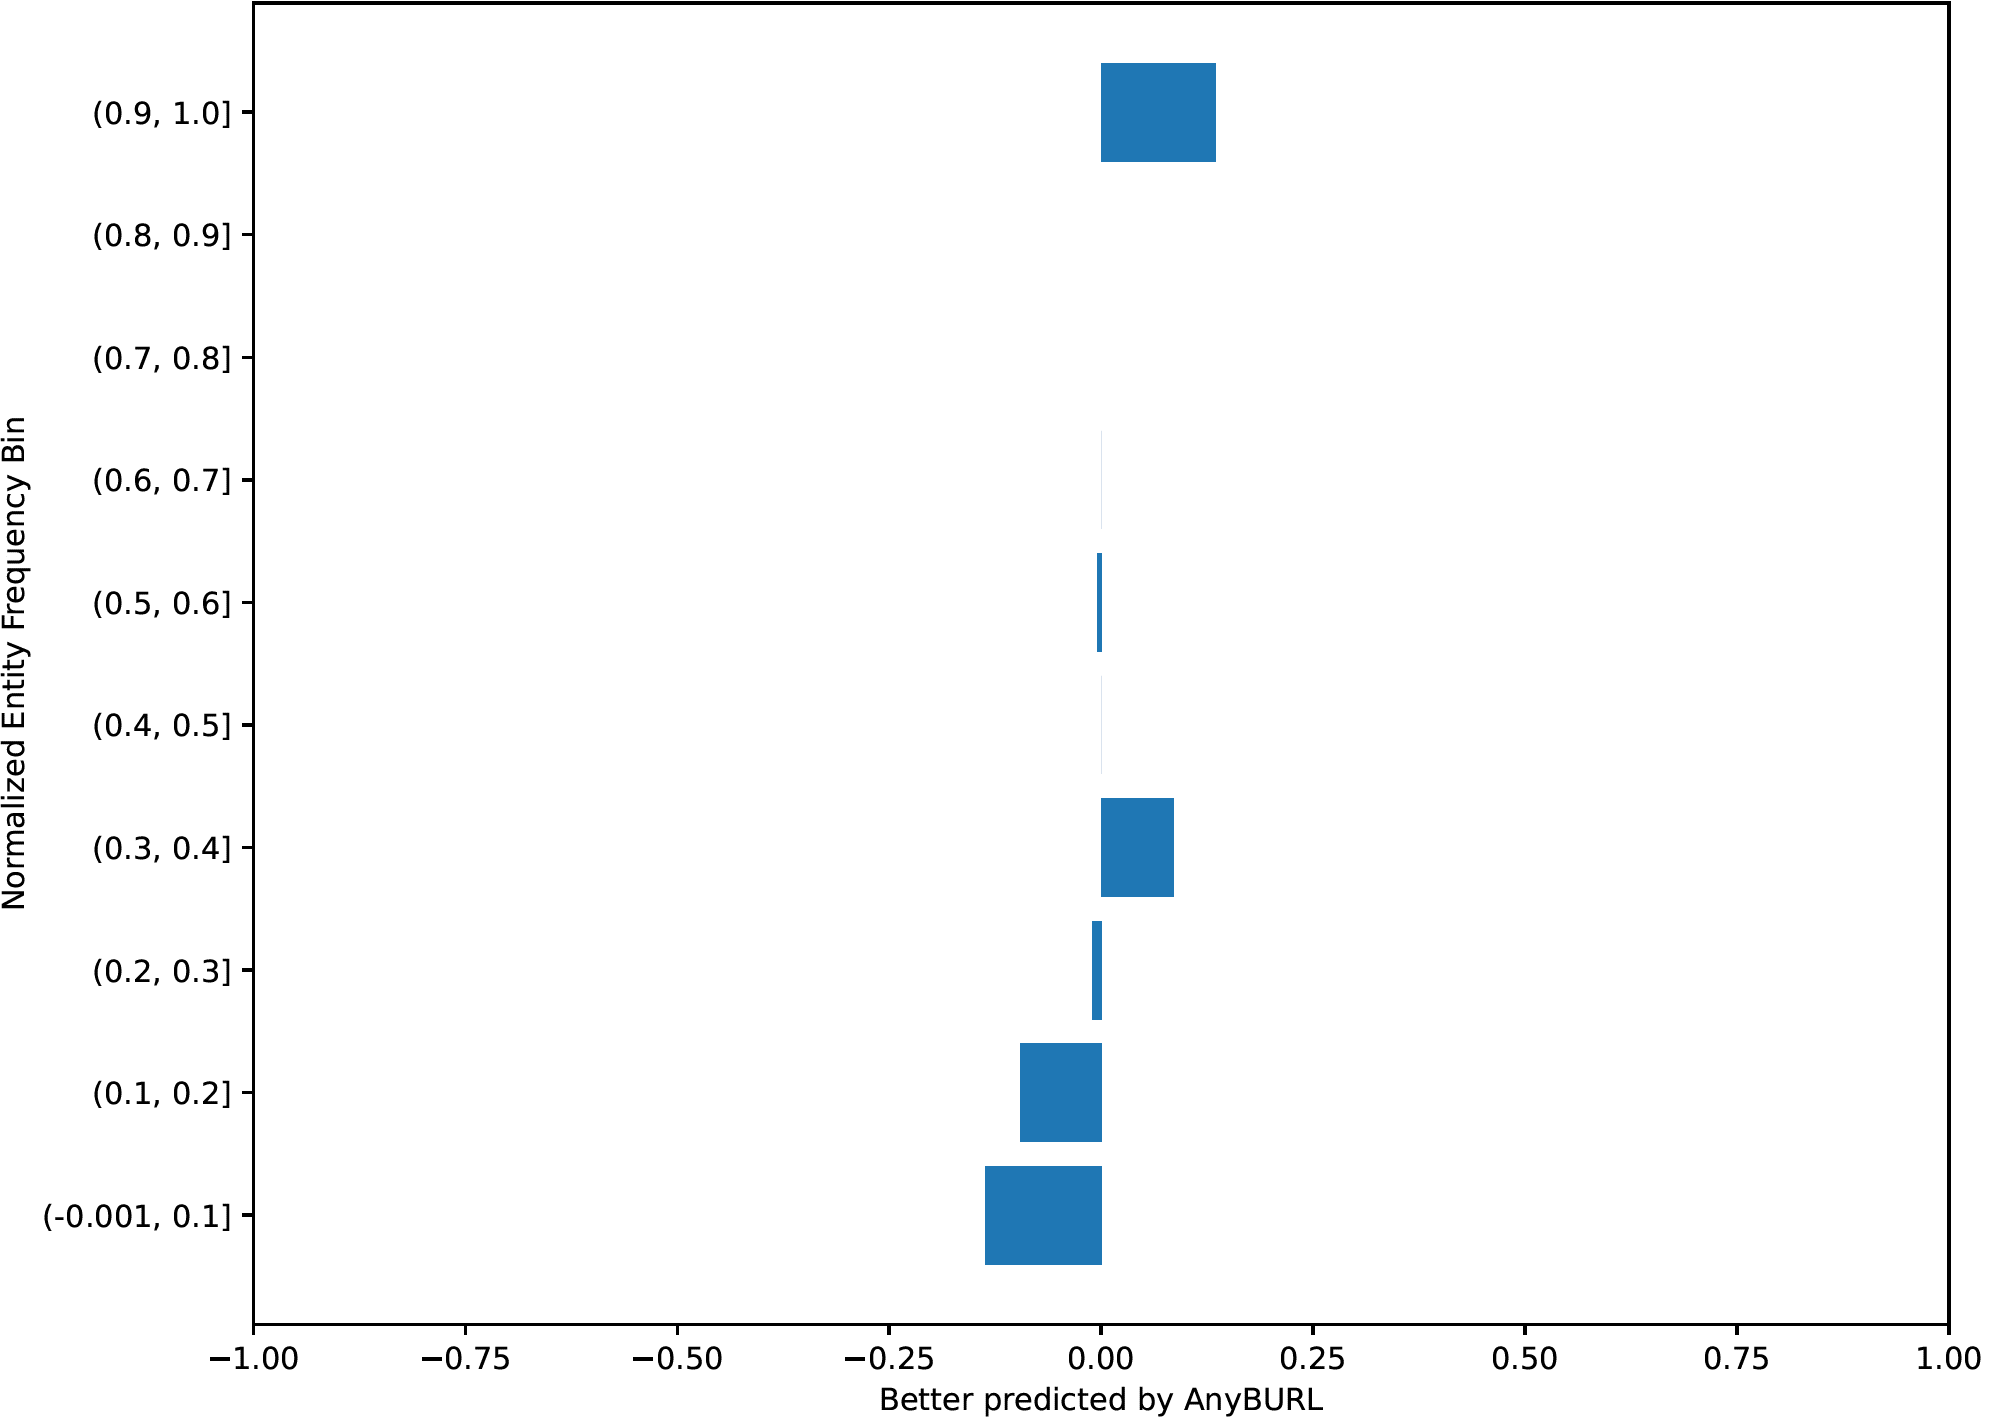
\includegraphics[width=0.7\textwidth]{images/entity_freq_answer_anyburl_conve_fb15k.PNG}
\caption{Comparison of AnyBURL and ConvE on FB15k-237 in regard to the answer entity frequency}
\label{fig:entity_answer_tail_anyburl_conve_fb15k}
\end{figure}

\begin{figure}[H]
\centering
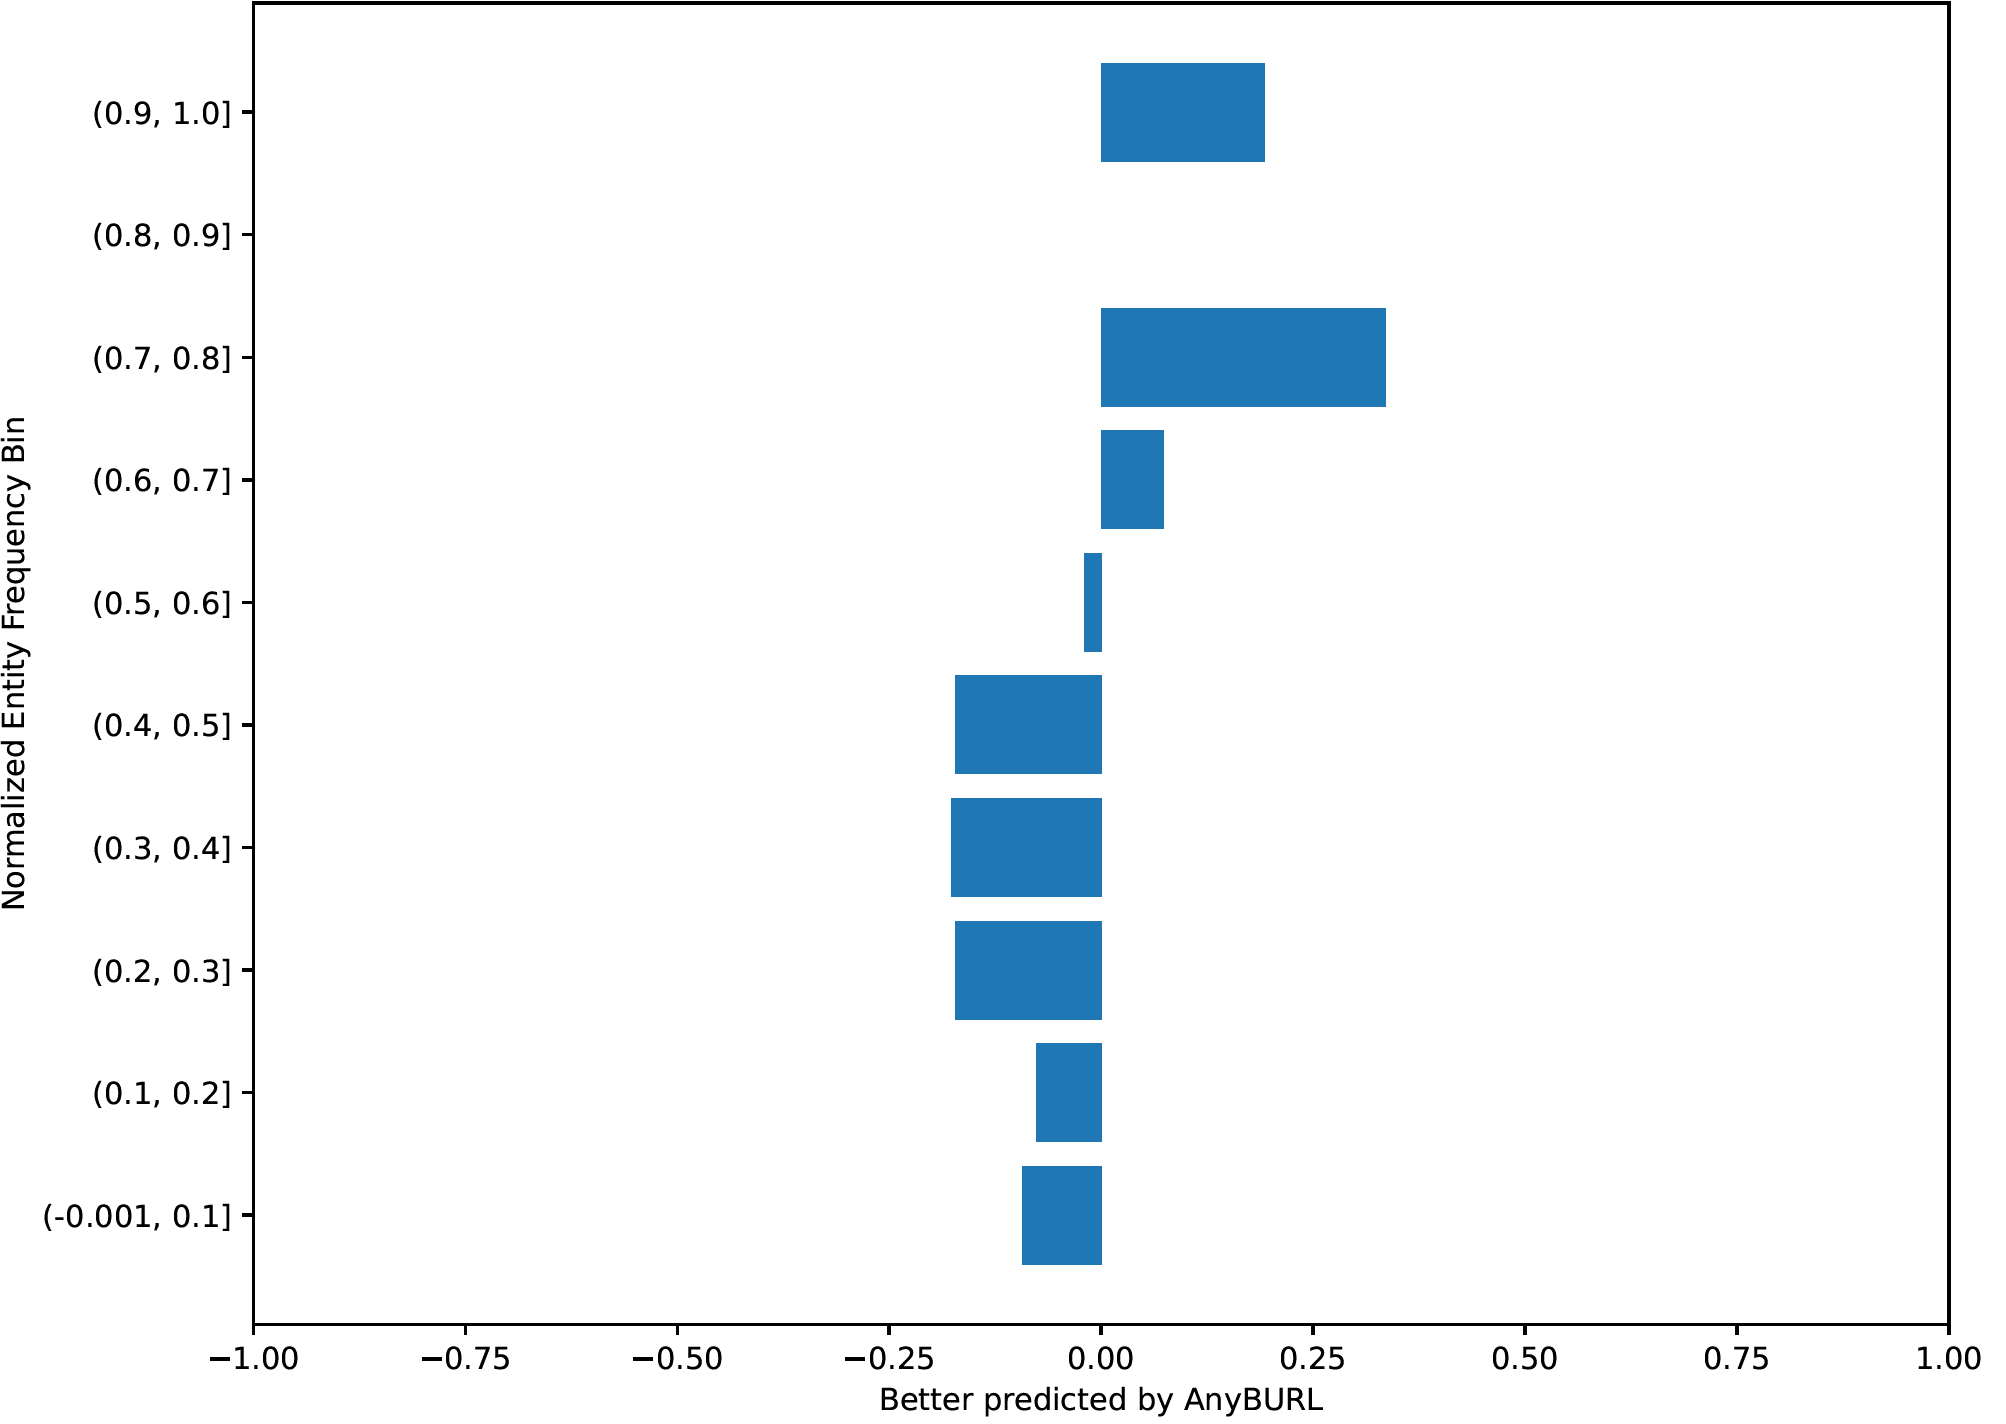
\includegraphics[width=0.7\textwidth]{images/combined_freq_anyburl_conve_fb15k.PNG}
\caption{Comparison of AnyBURL and ConvE on FB15k-237 in regard to the combined entity and relation frequency}
\label{fig:combined_freq_anyburl_conve_fb15k}
\end{figure}




\subsection{AnyBURL and RESCAL on FB15k-237}

\begin{figure}[H]
\centering
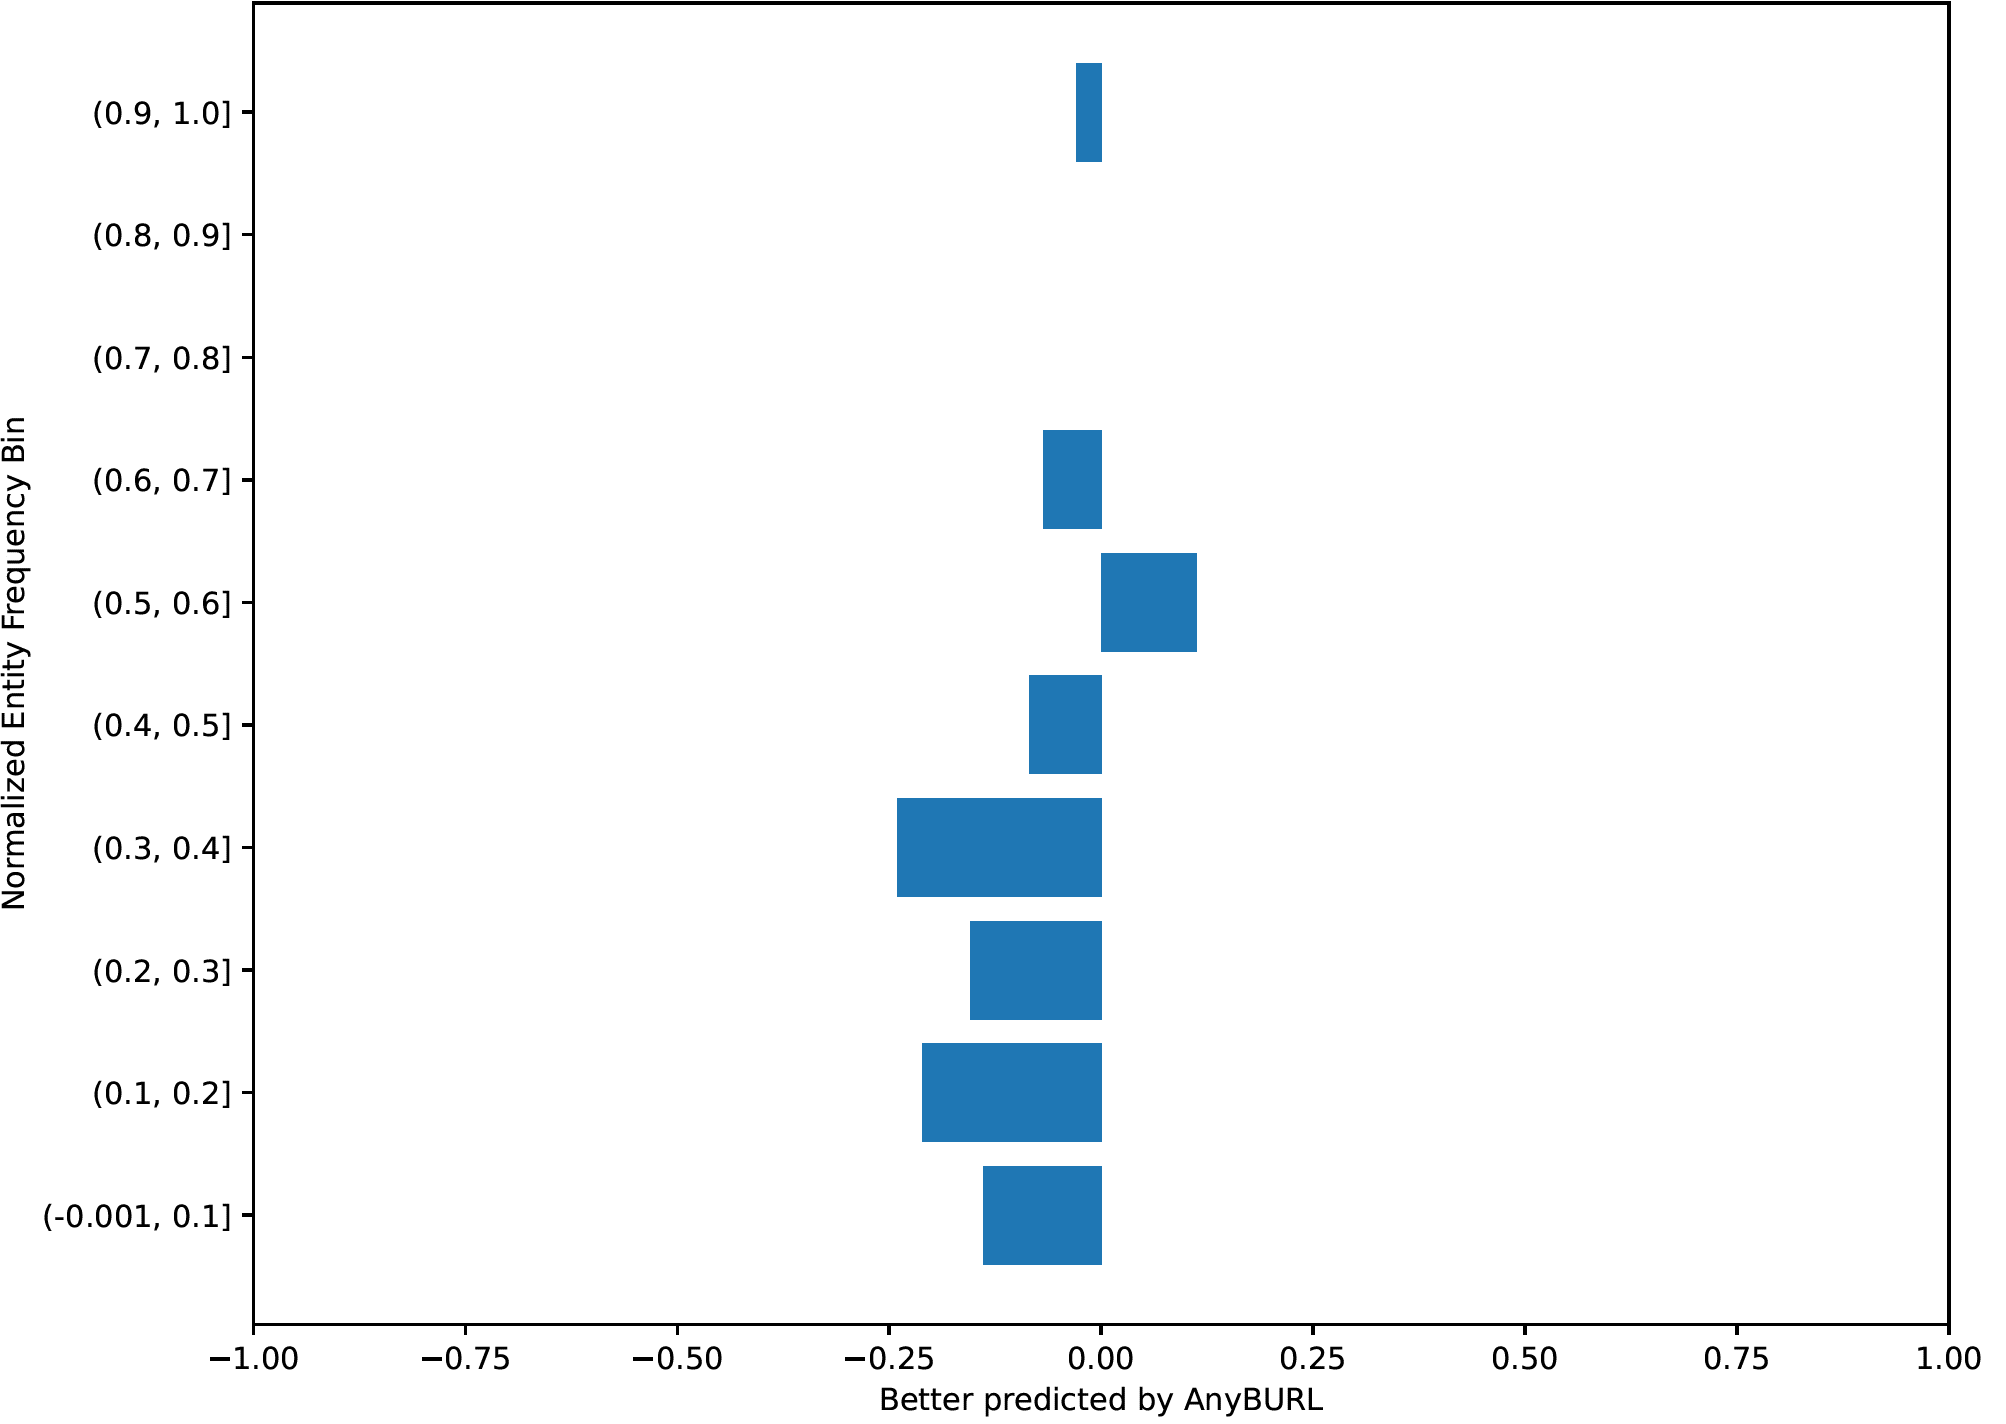
\includegraphics[width=0.7\textwidth]{images/entity_freq_question_anyburl_rescal_fb15k.PNG}
\caption{Comparison of AnyBURL and RESCAL on FB15k-237 in regard to the question entity frequency}
\label{fig:entity_question_tail_anyburl_rescal_fb15k}
\end{figure}

\begin{figure}[H]
\centering
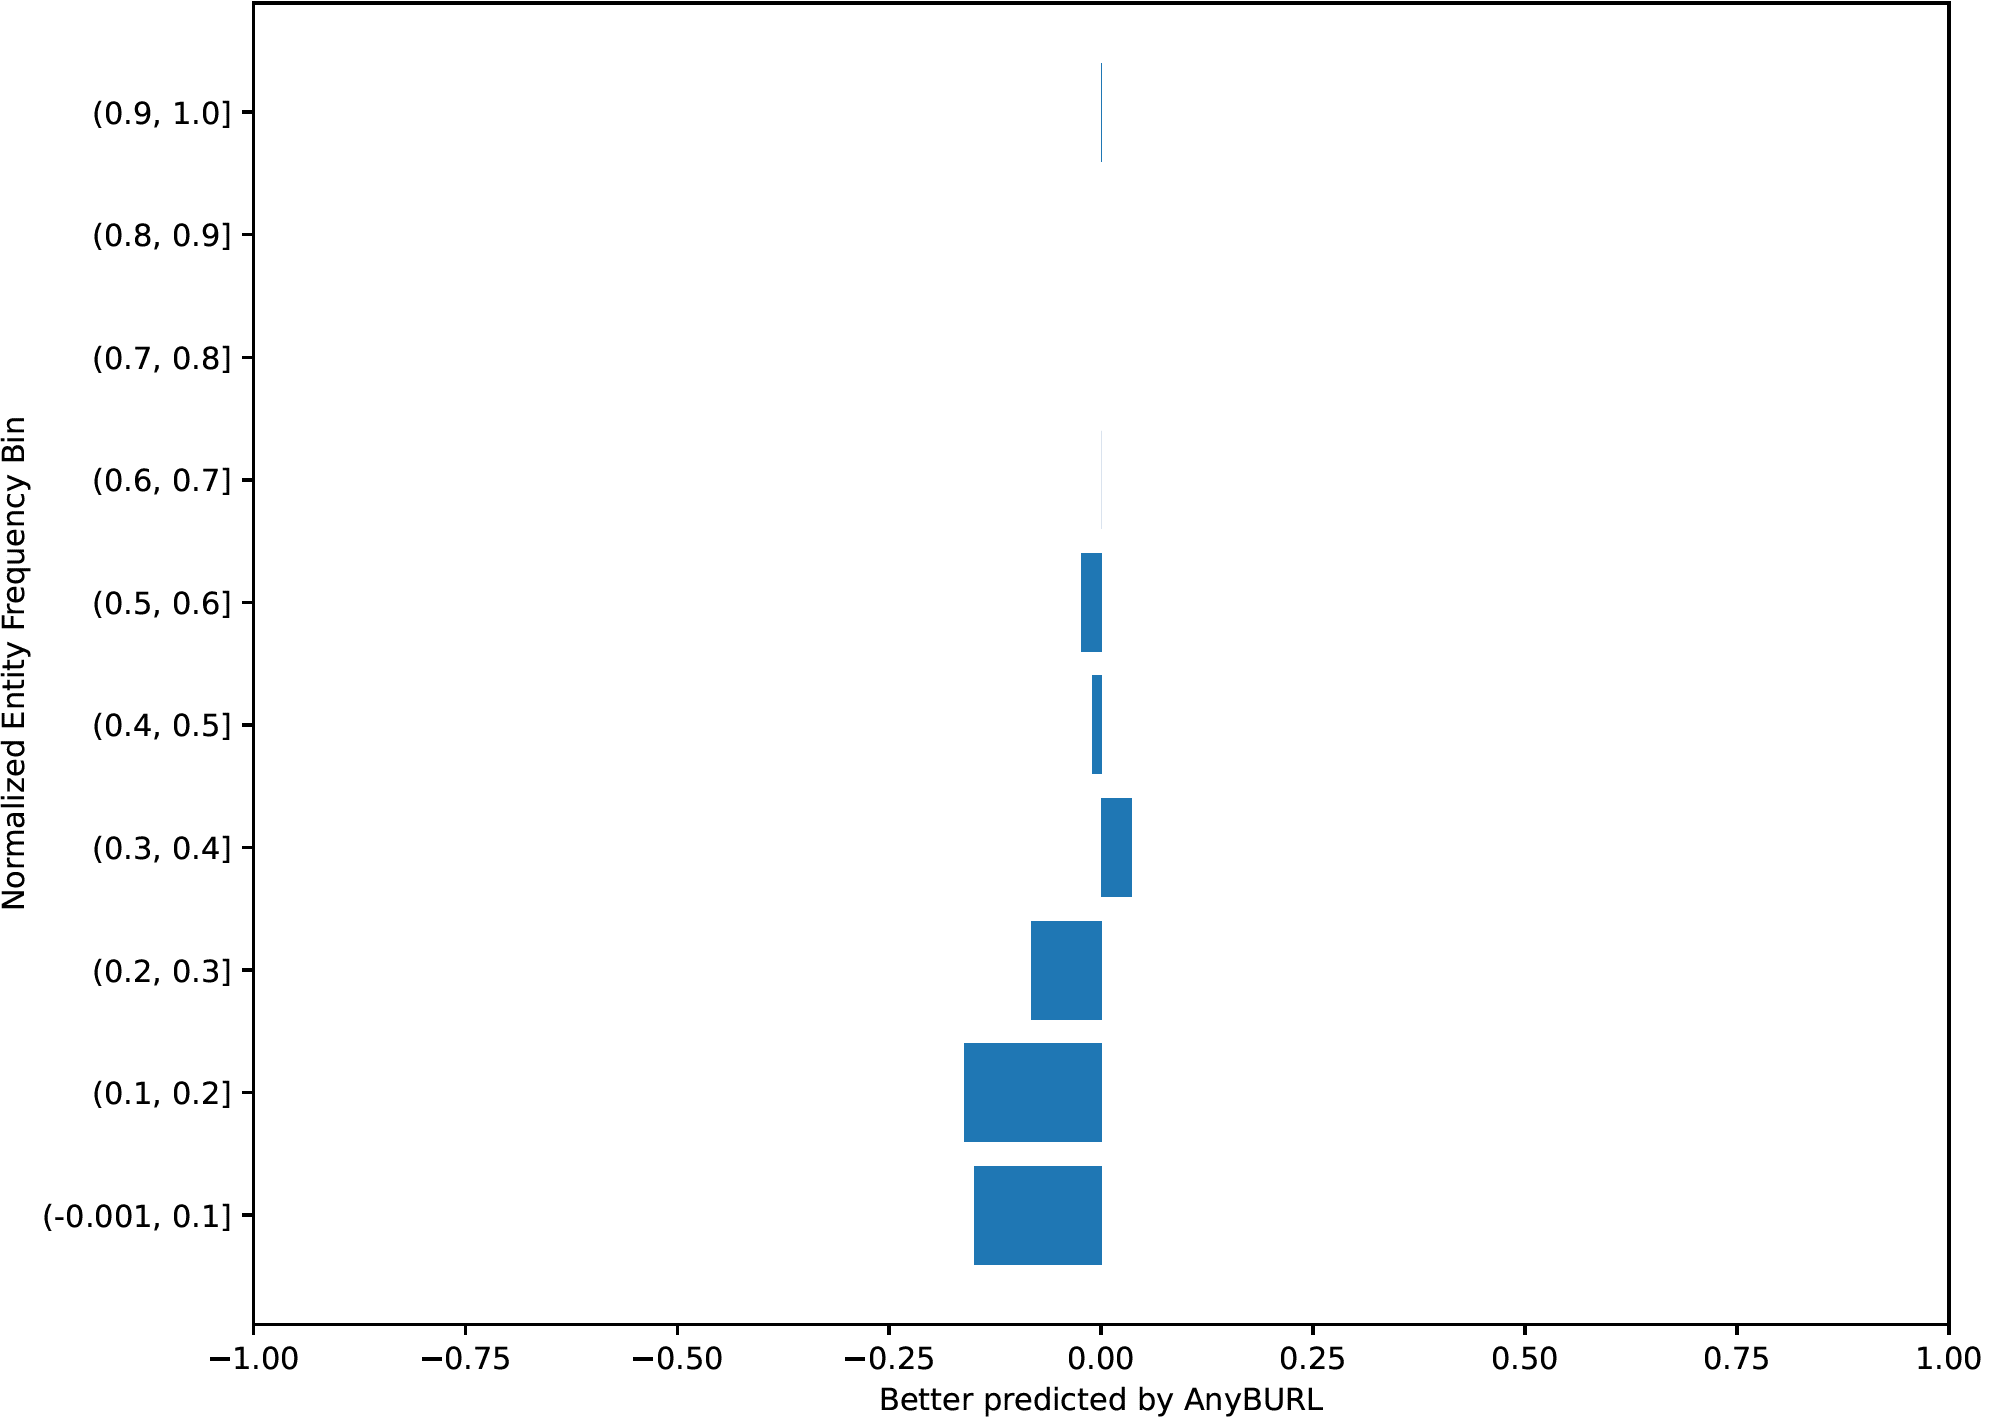
\includegraphics[width=0.7\textwidth]{images/entity_freq_answer_anyburl_rescal_fb15k.PNG}
\caption{Comparison of AnyBURL and RESCAL on FB15k-237 in regard to the answer entity frequency}
\label{fig:entity_answer_tail_anyburl_rescal_fb15k}
\end{figure}

\begin{figure}[H]
\centering
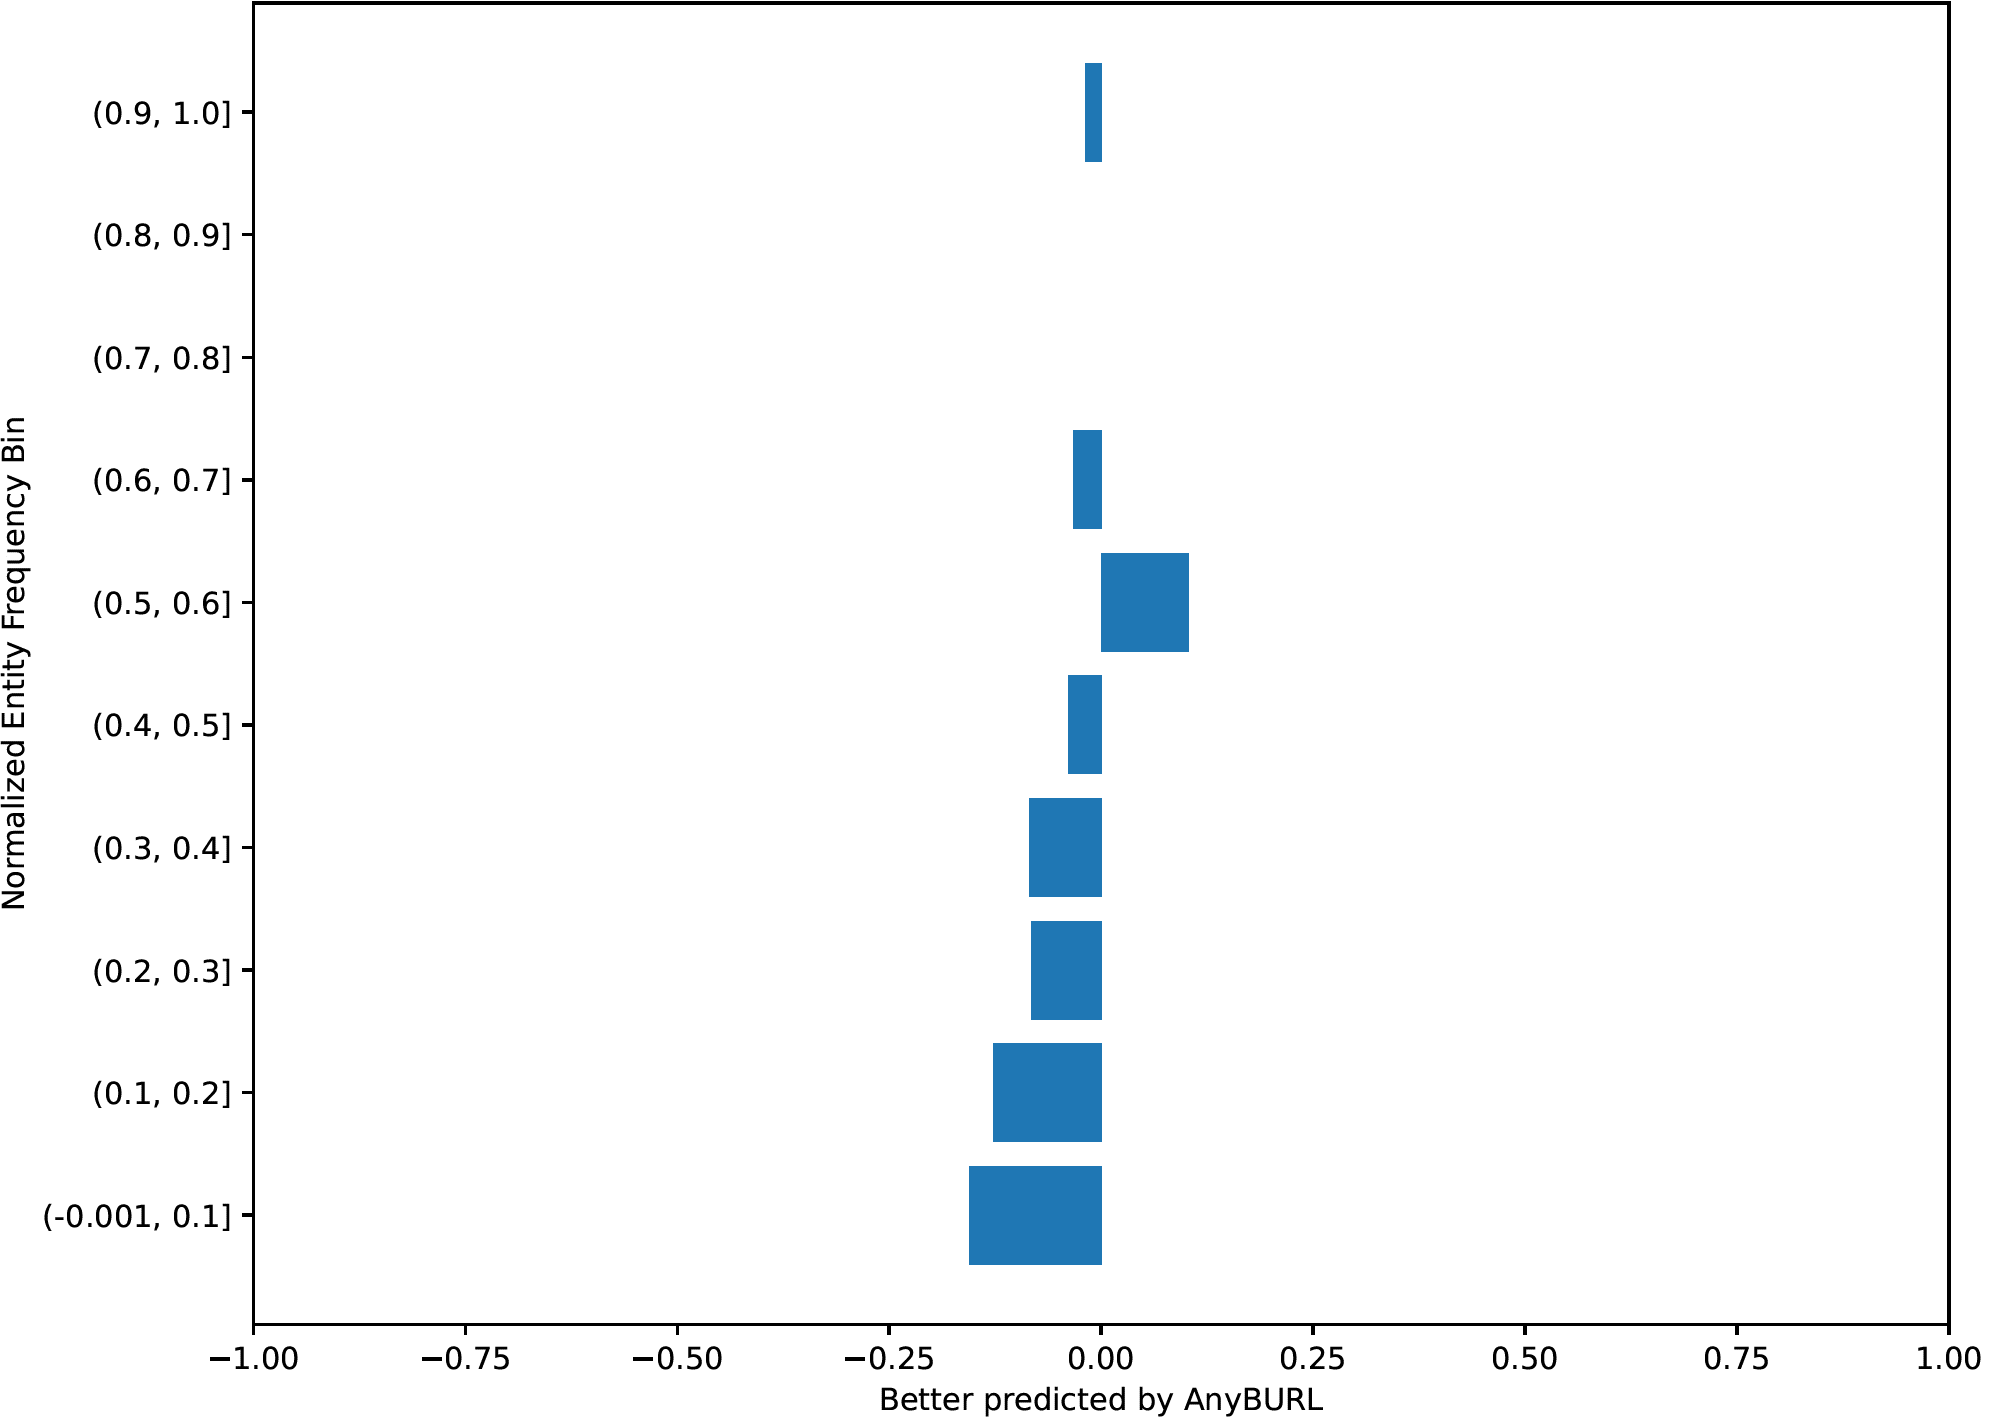
\includegraphics[width=0.7\textwidth]{images/combined_freq_anyburl_rescal_fb15k.PNG}
\caption{Comparison of AnyBURL and RESCAL on FB15k-237 in regard to the combined entity and relation frequency}
\label{fig:combined_freq_anyburl_rescal_fb15k}
\end{figure}



\subsection{AnyBURL and ComplEx on YAGO3-10}

\begin{figure}[H]
\centering
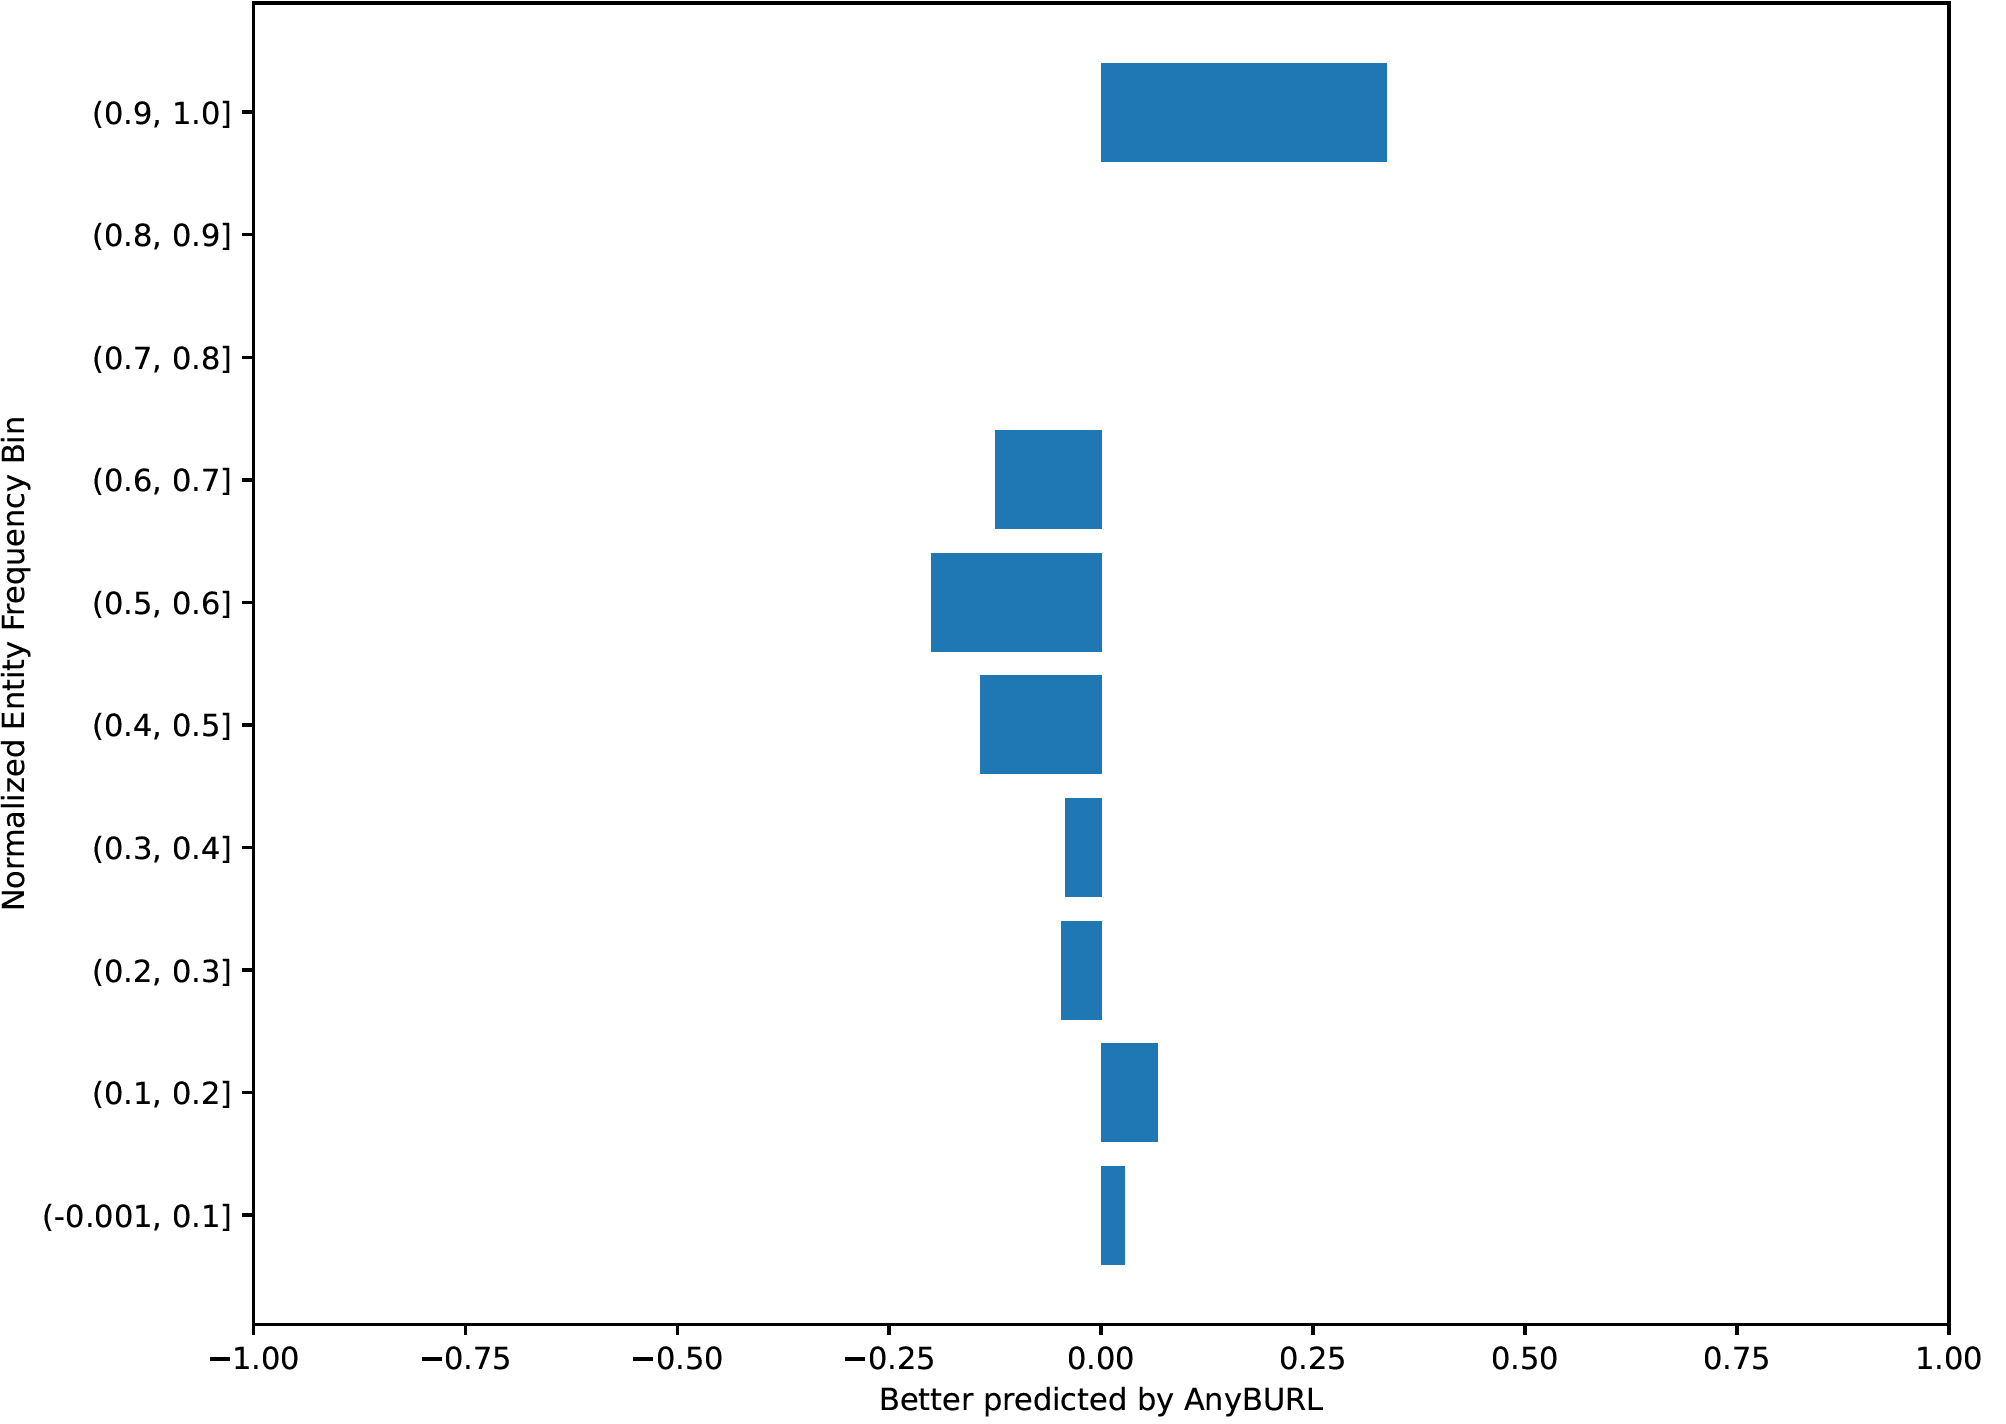
\includegraphics[width=0.7\textwidth]{images/entity_freq_question_anyburl_complex_yago.PNG}
\caption{Comparison of AnyBURL and ComplEx on YAGO3-10 in regard to the question entity frequency}
\label{fig:entity_question_tail_anyburl_complex_yago}
\end{figure}

\begin{figure}[H]
\centering
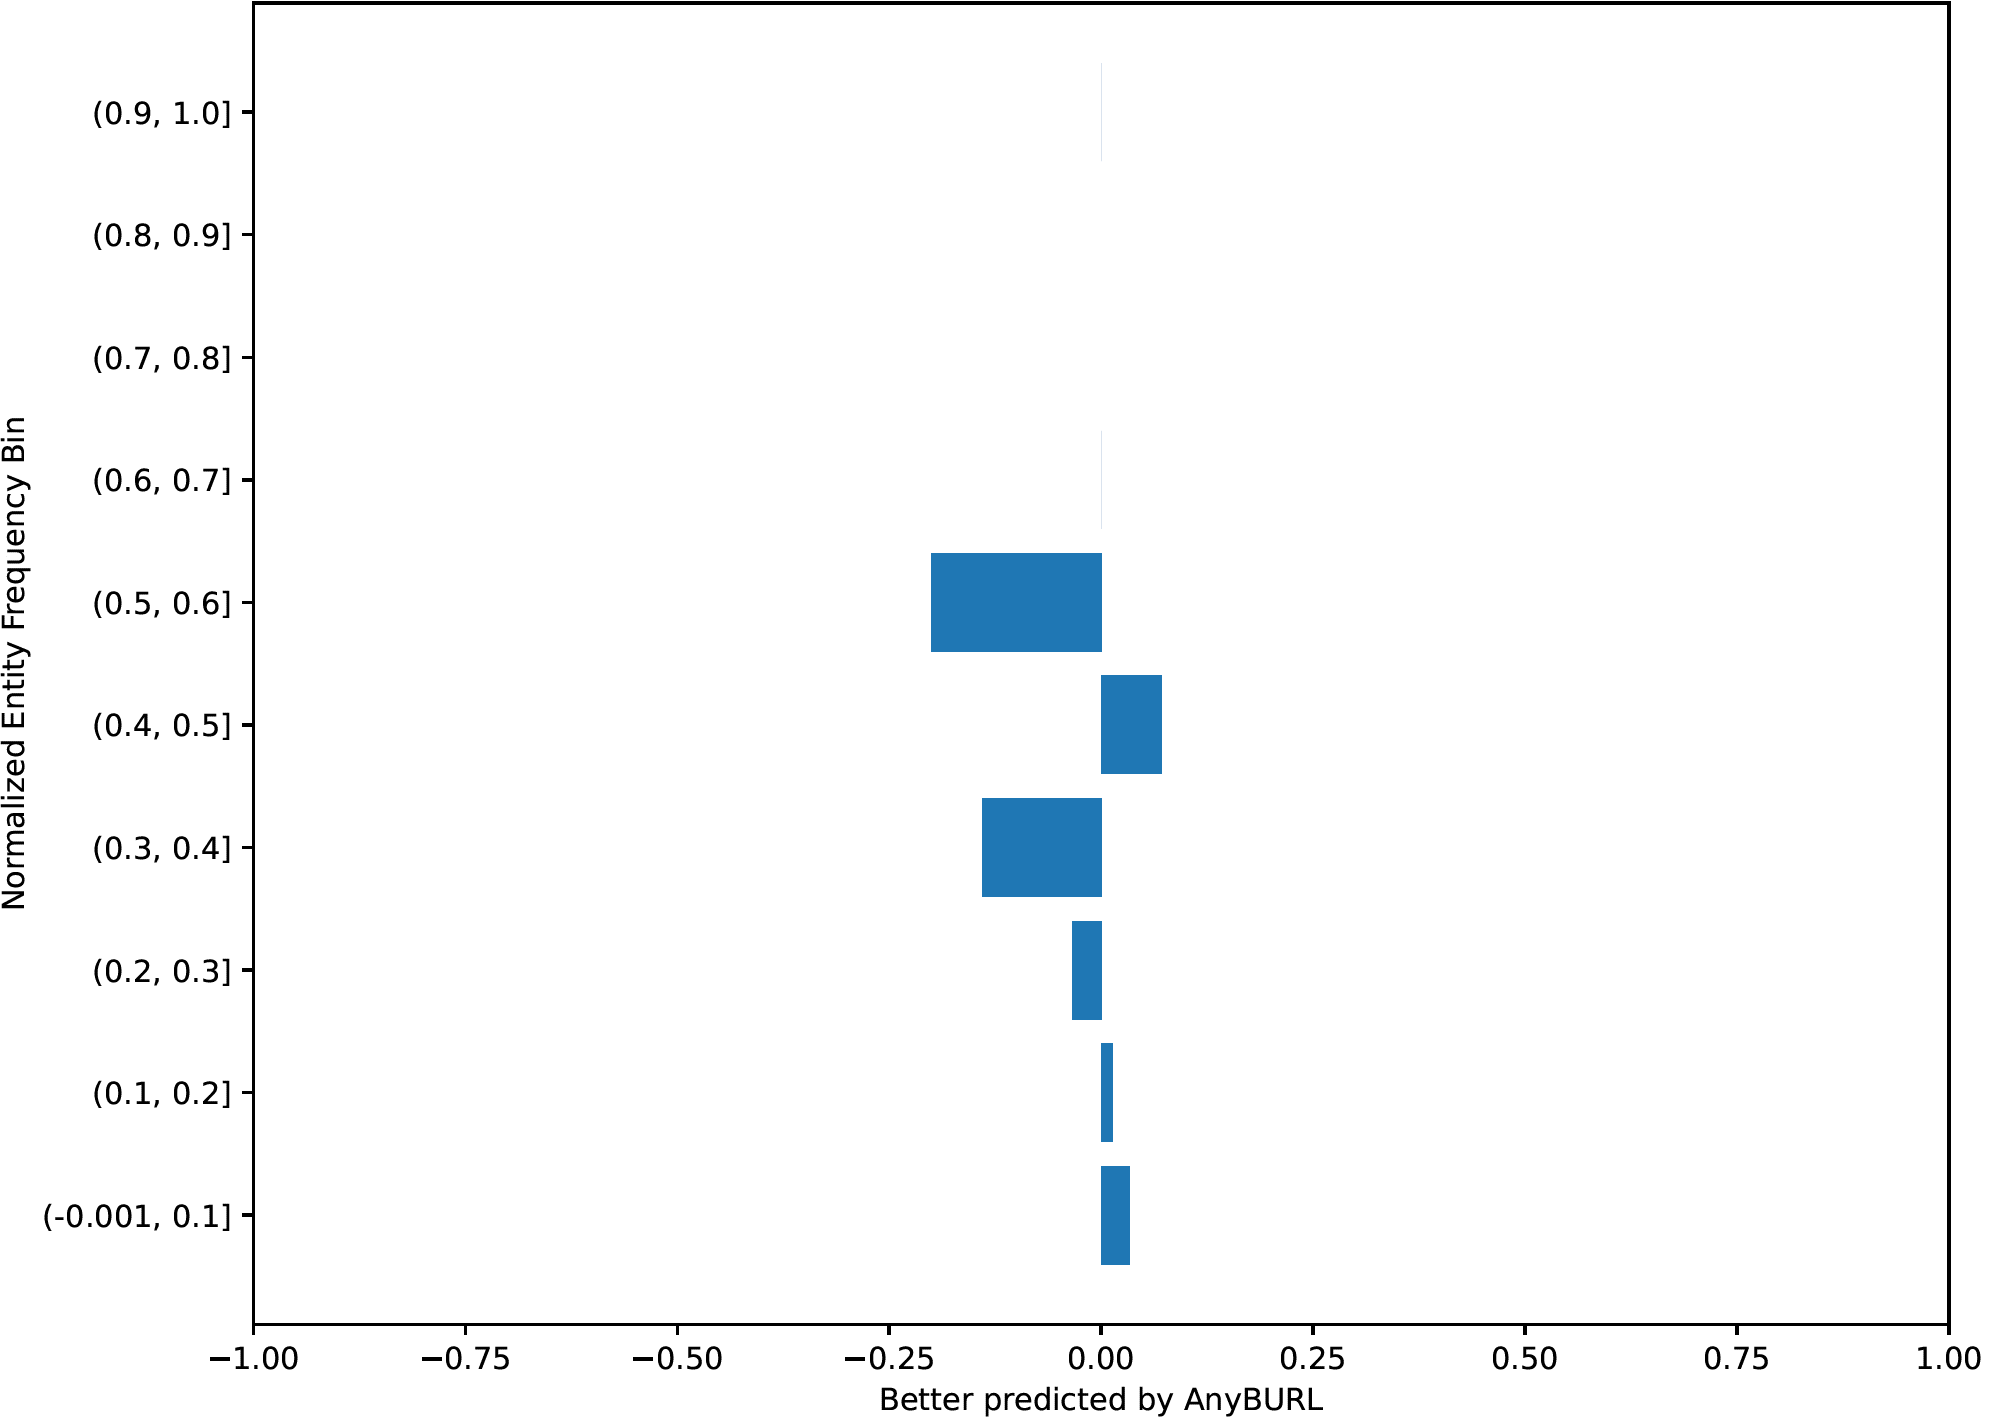
\includegraphics[width=0.7\textwidth]{images/entity_freq_answer_anyburl_complex_yago.PNG}
\caption{Comparison of AnyBURL and ComplEx on YAGO3-10 in regard to the answer entity frequency}
\label{fig:entity_answer_tail_anyburl_complex_yago}
\end{figure}

\begin{figure}[H]
\centering
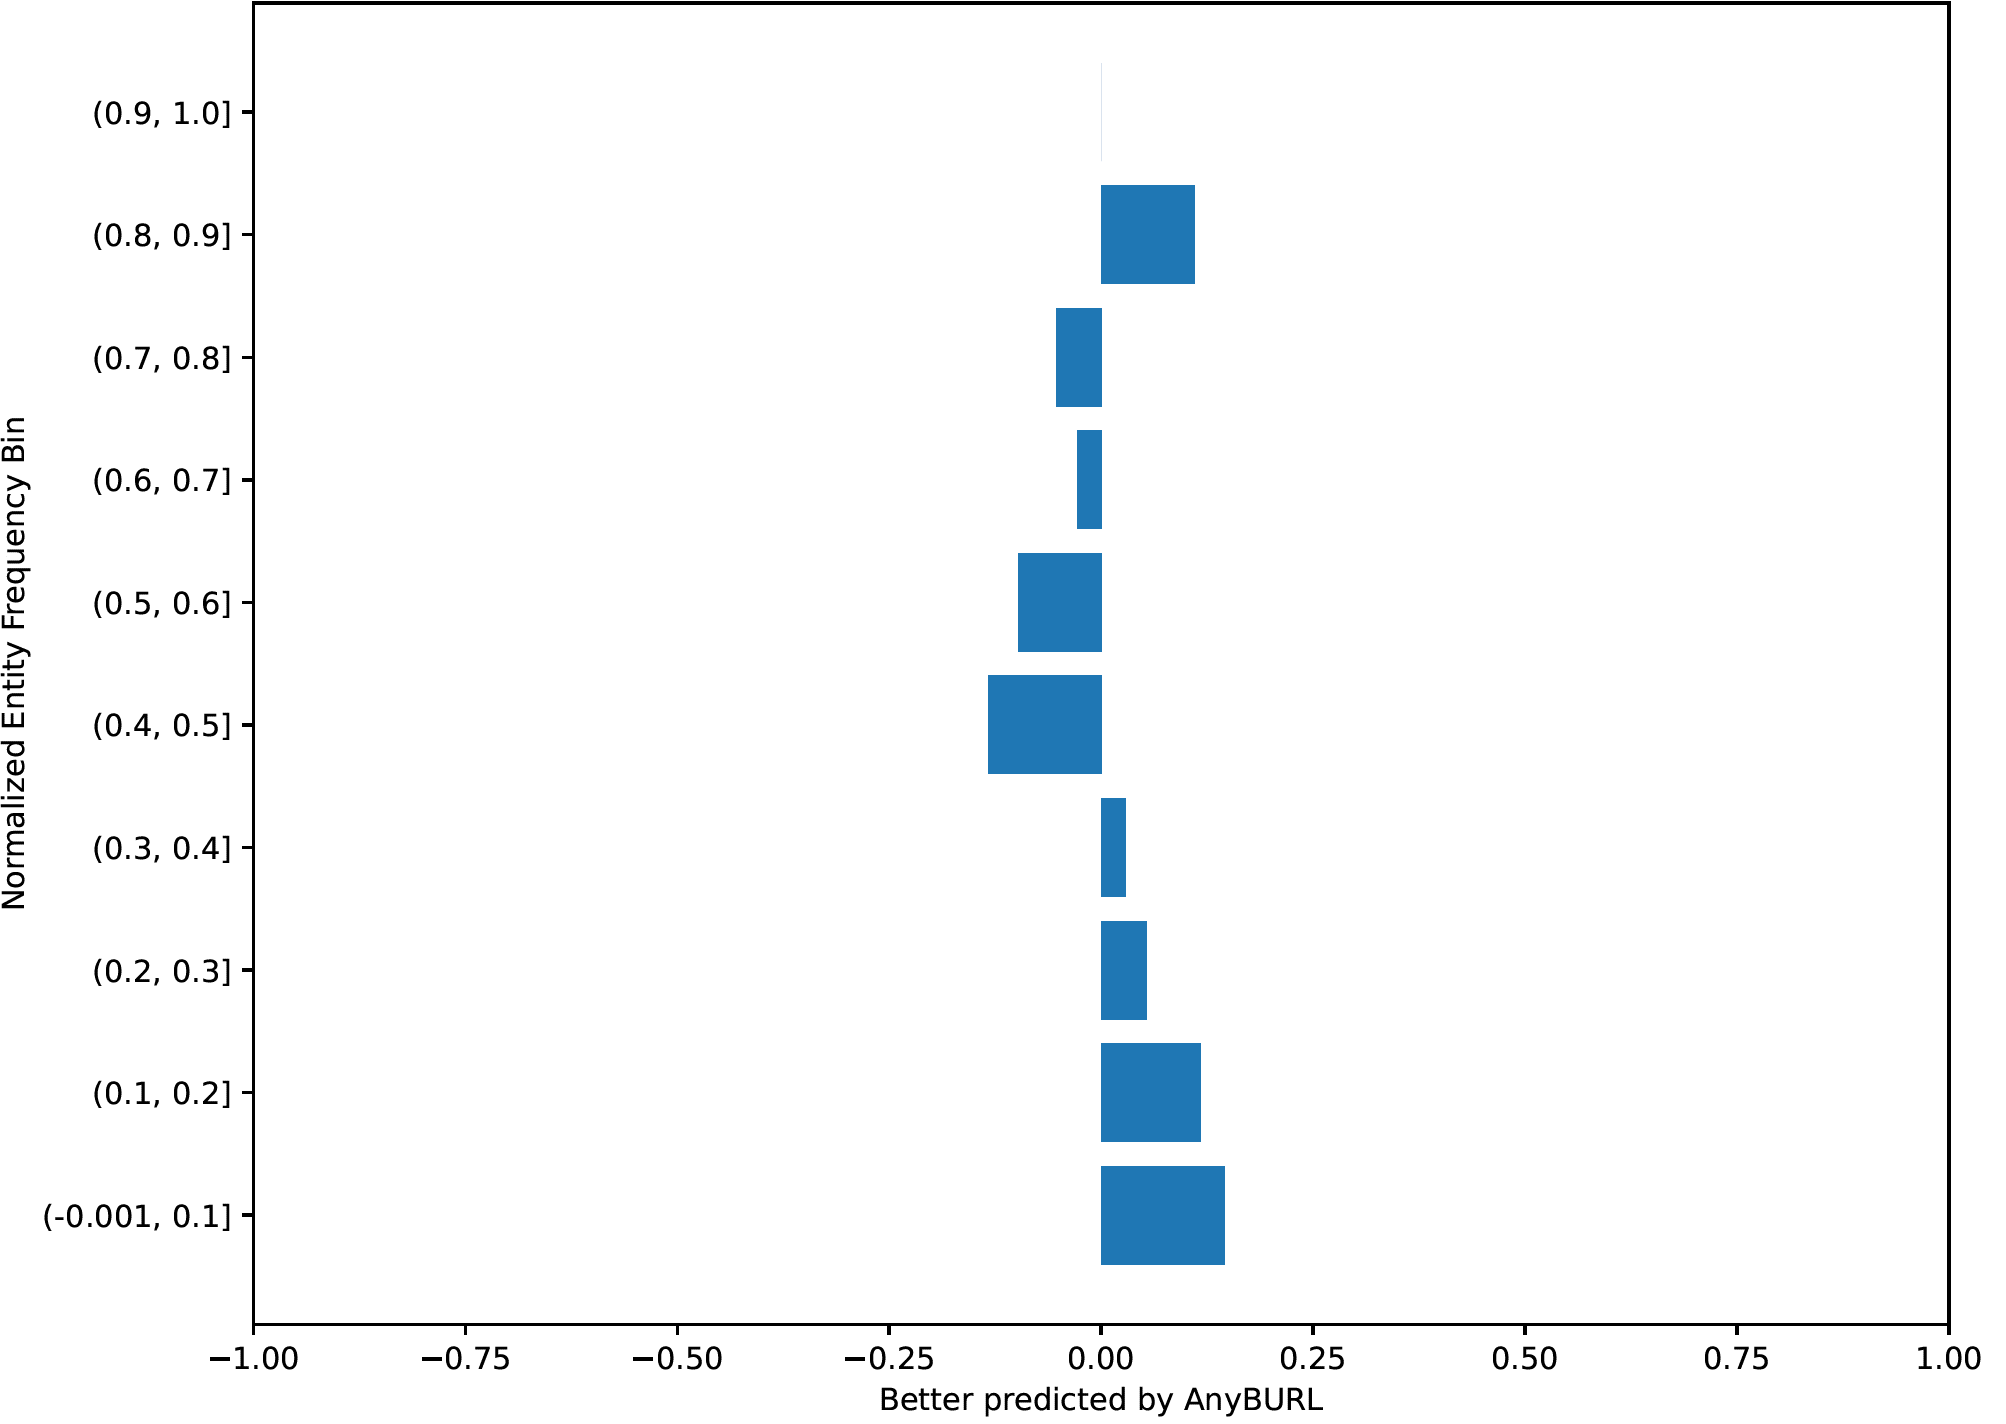
\includegraphics[width=0.7\textwidth]{images/combined_freq_anyburl_complex_yago.PNG}
\caption{Comparison of AnyBURL and ComplEx on YAGO3-10 in regard to the combined entity and relation frequency}
\label{fig:combined_freq_anyburl_complex_yago}
\end{figure}
\section{Comparison in regard to the Existence of Similar Triples in the Trainings Data}
\label{appendix:similar_triples}

\subsection{Binary}

\begin{figure}[H]
\centering
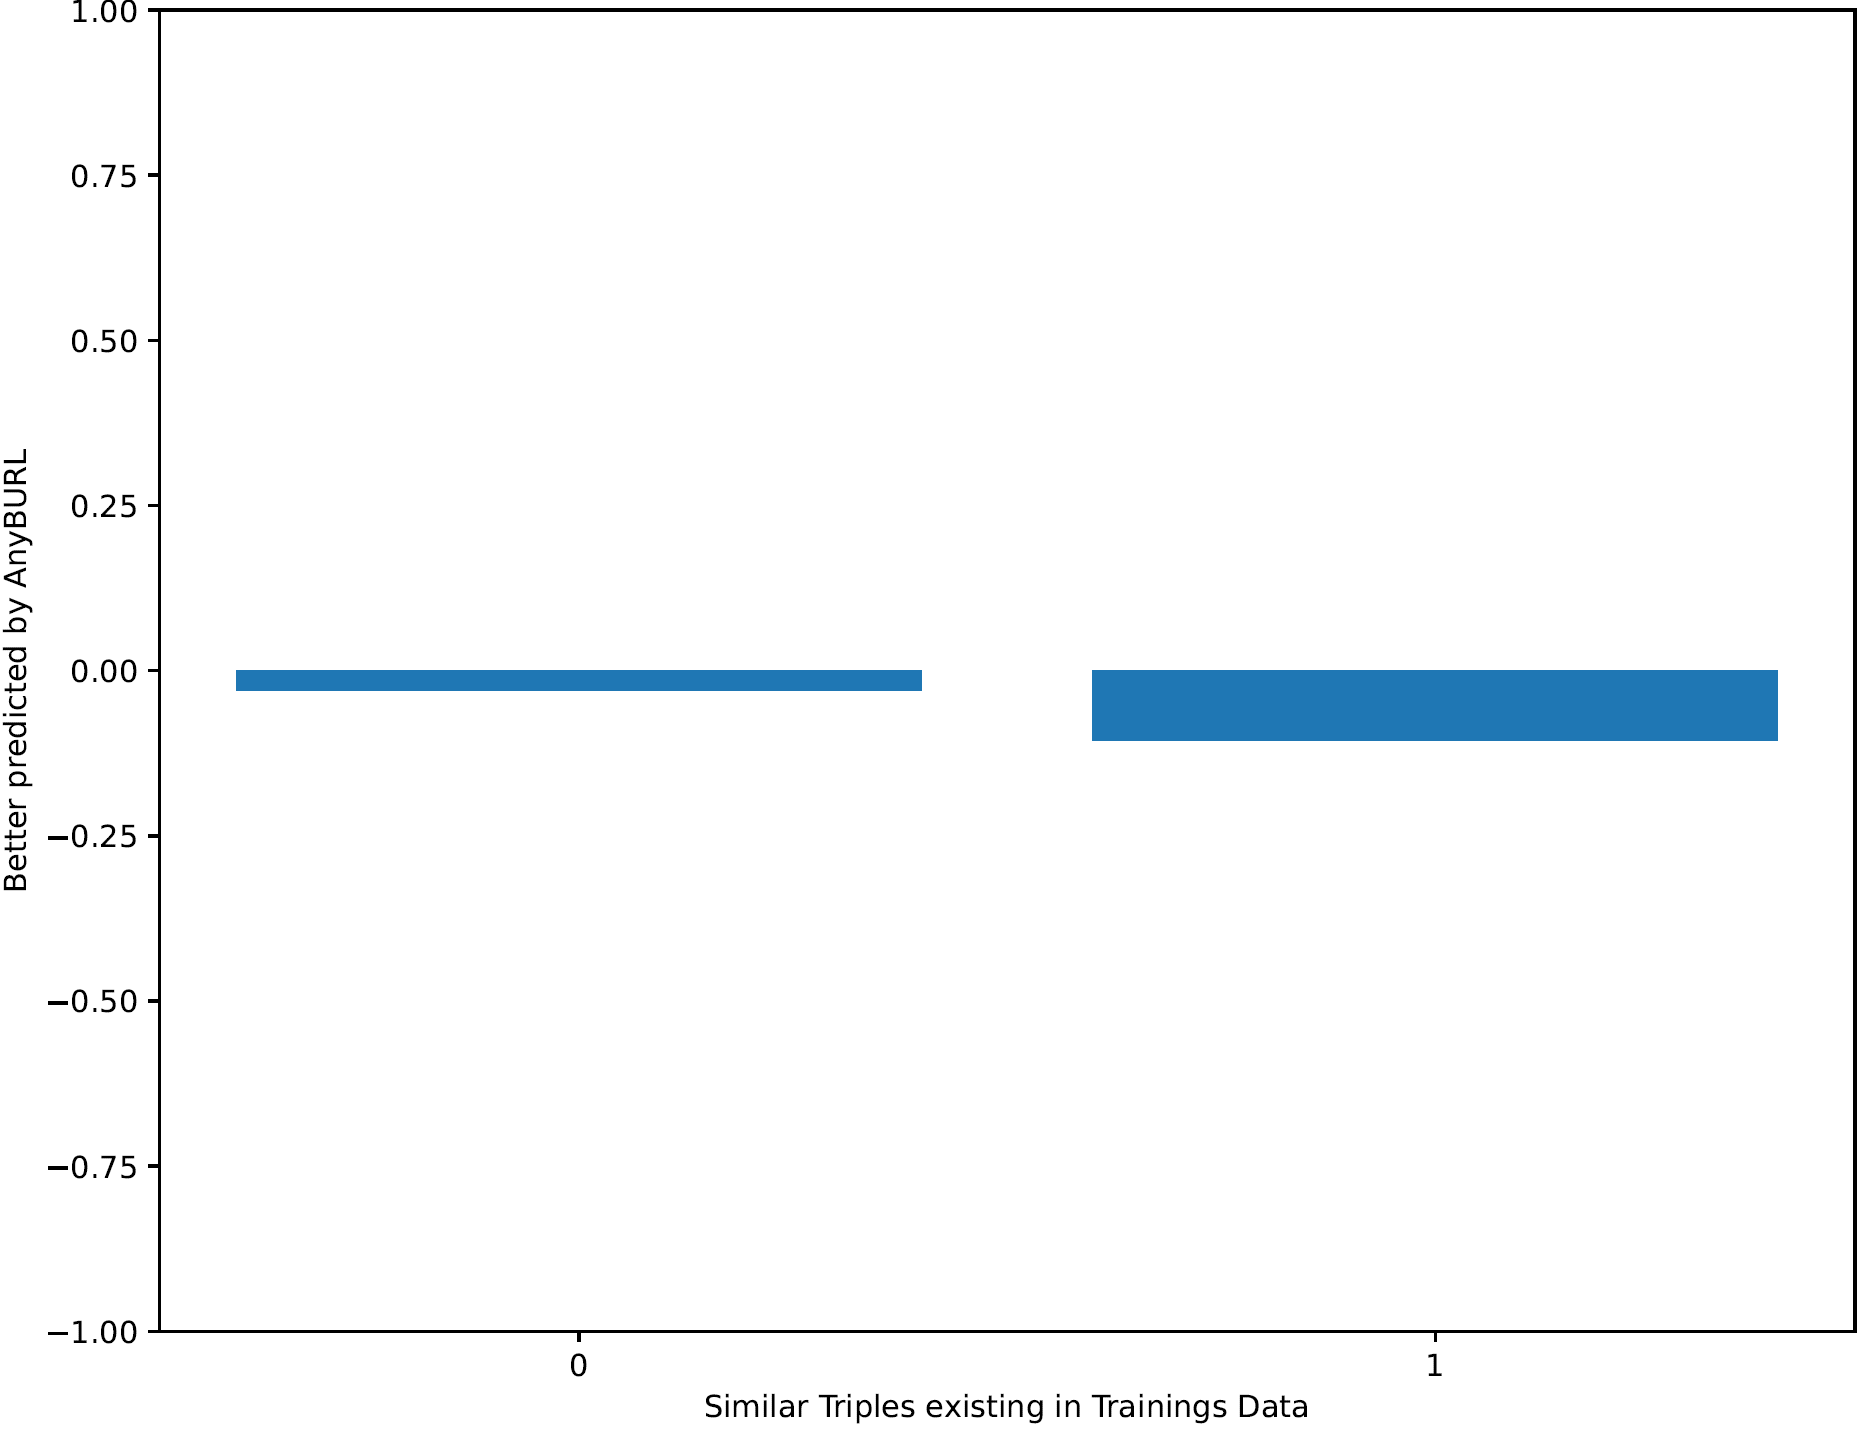
\includegraphics[width=0.7\textwidth]{images/similar_triples_binary_anyburl_conve_codex.PNG}
\caption{Comparison of AnyBURL and ConvE on FB15k-237 in regard to the existence of similar triples in the trainings data}
\label{fig:similar_triples_binary_anyburl_conve_fb15k}
\end{figure}

\begin{figure}[H]
\centering
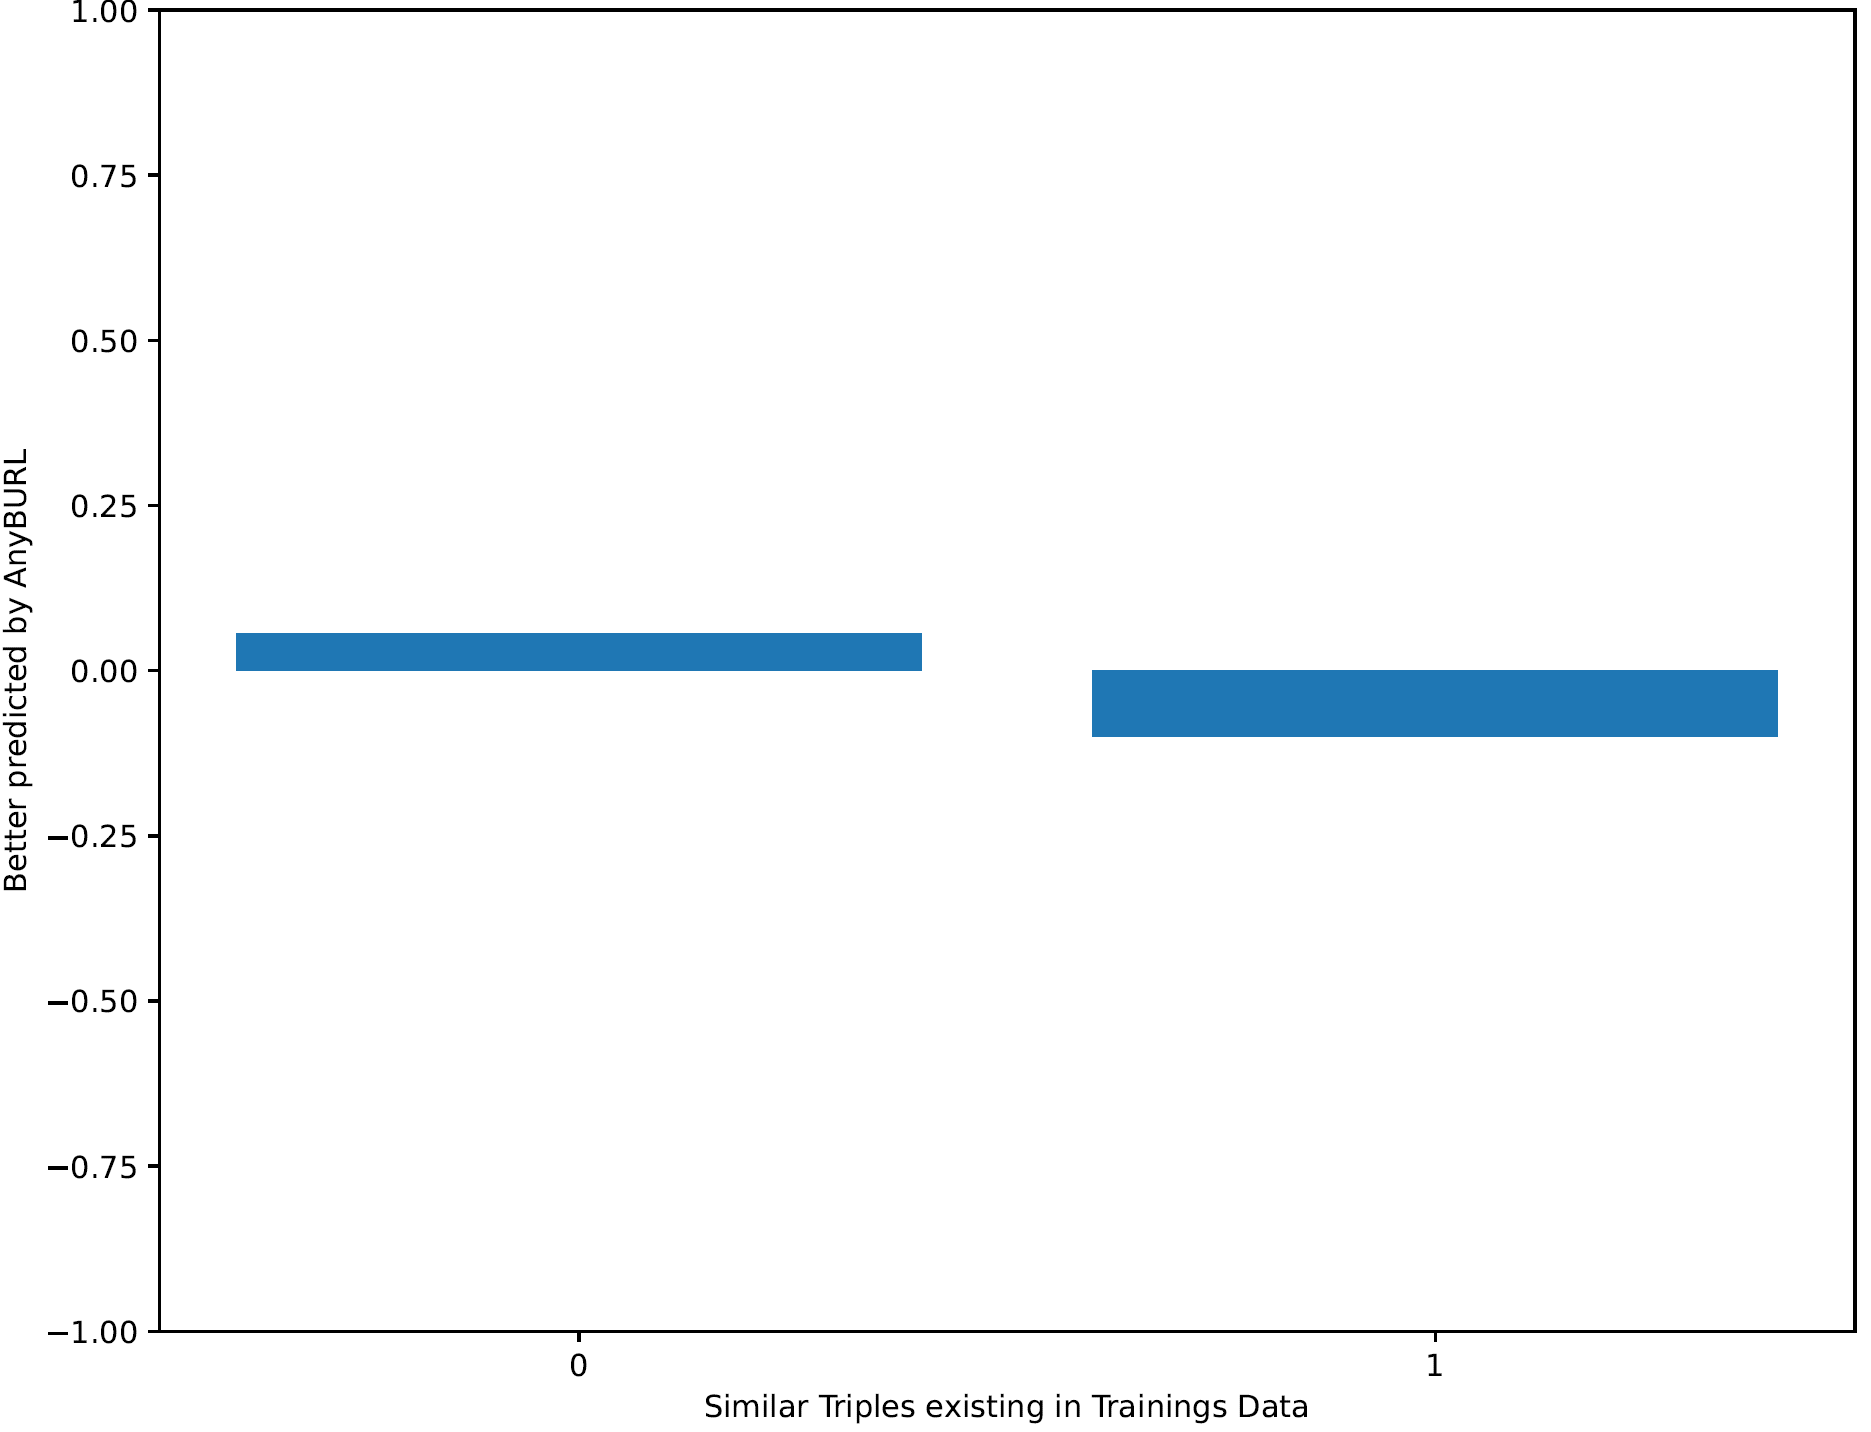
\includegraphics[width=0.7\textwidth]{images/similar_triples_binary_anyburl_rescal_codex.PNG}
\caption{Comparison of AnyBURL and RESCAL on FB15k-237 in regard to the existence of similar triples in the trainings data}
\label{fig:similar_triples_binary_anyburl_rescal_fb15k}
\end{figure}

\begin{figure}[H]
\centering
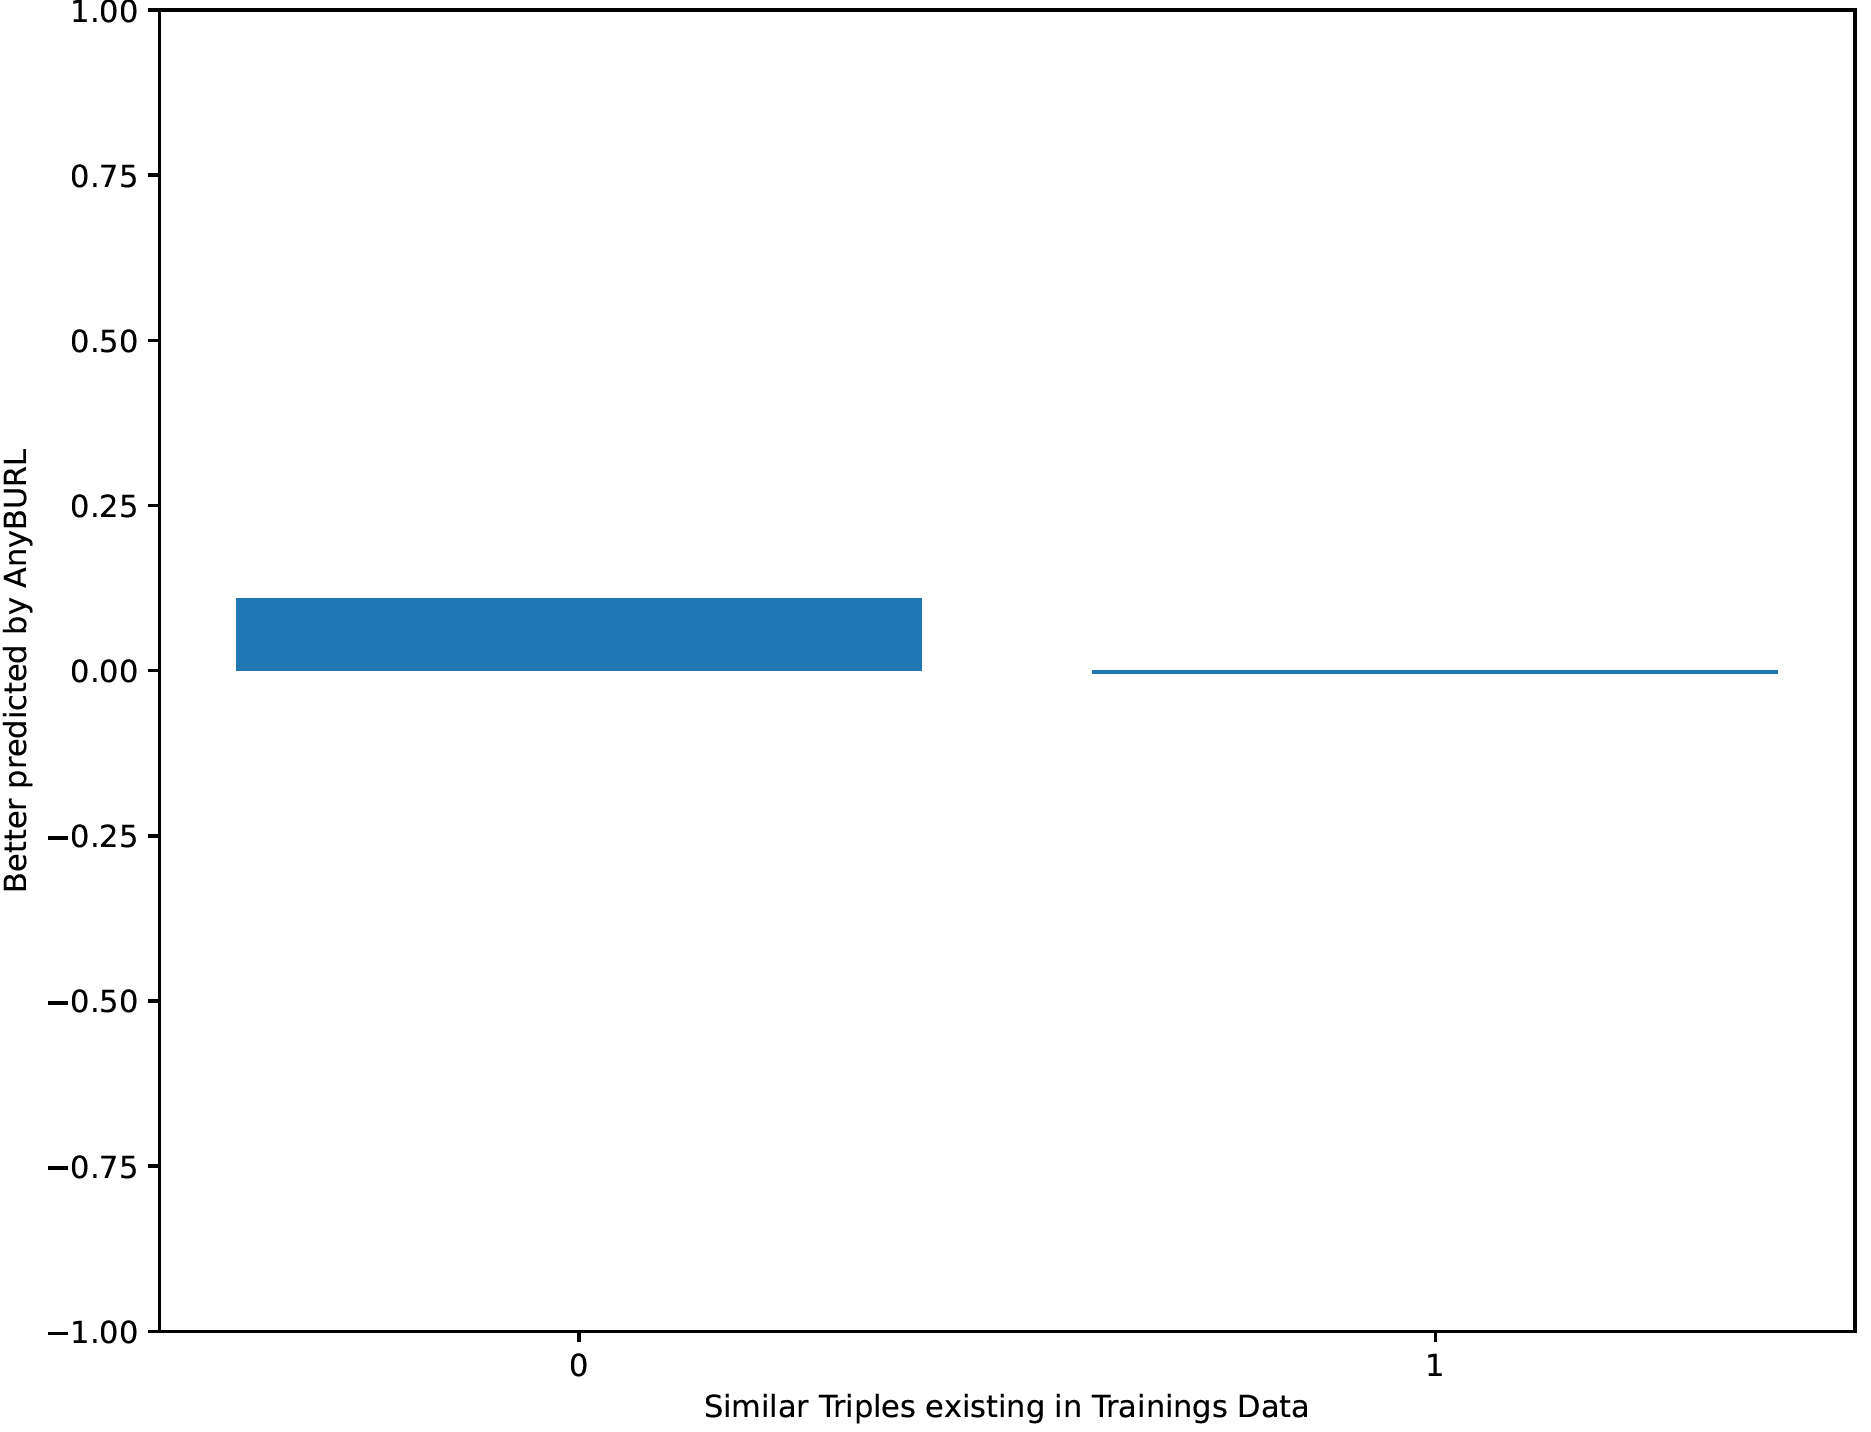
\includegraphics[width=0.7\textwidth]{images/similar_triples_binary_anyburl_complex_yago.PNG}
\caption{Comparison of AnyBURL and ComplEx on YAGO3-10 in regard to the existence of similar triples in the trainings data}
\label{fig:similar_triples_binary_anyburl_complex_yago}
\end{figure}

\subsection{Stepwise}

\begin{figure}[H]
\centering
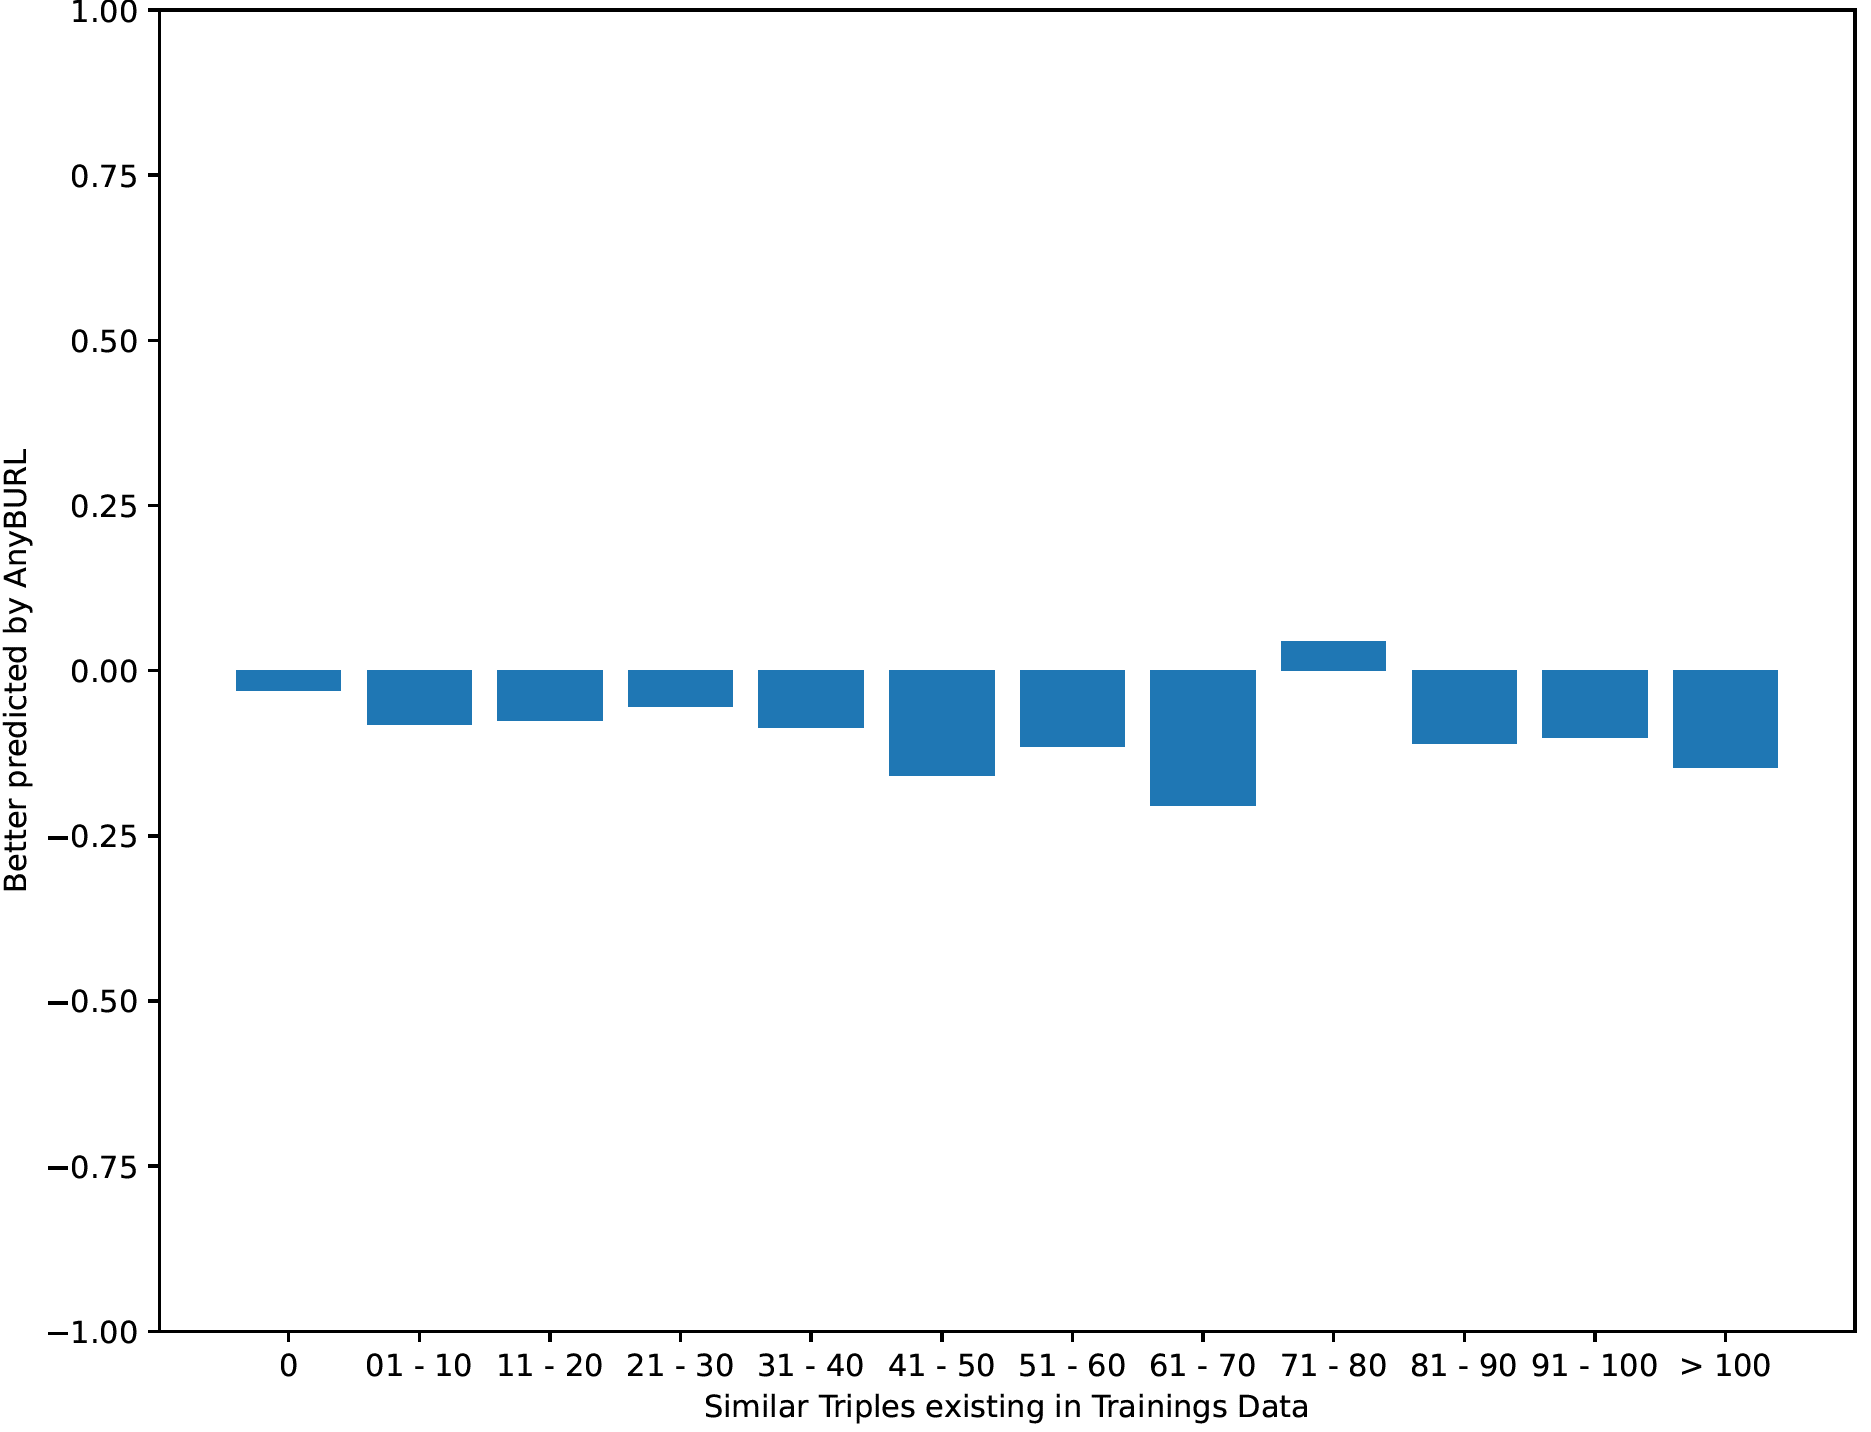
\includegraphics[width=0.7\textwidth]{images/similar_triples_steps_anyburl_conve_codex.PNG}
\caption{Comparison of AnyBURL and ConvE on CodEx-M in regard to the amount of similar triples in the trainings data}
\label{fig:similar_triples_steps_anyburl_conve_codex}
\end{figure}

\begin{figure}[H]
\centering
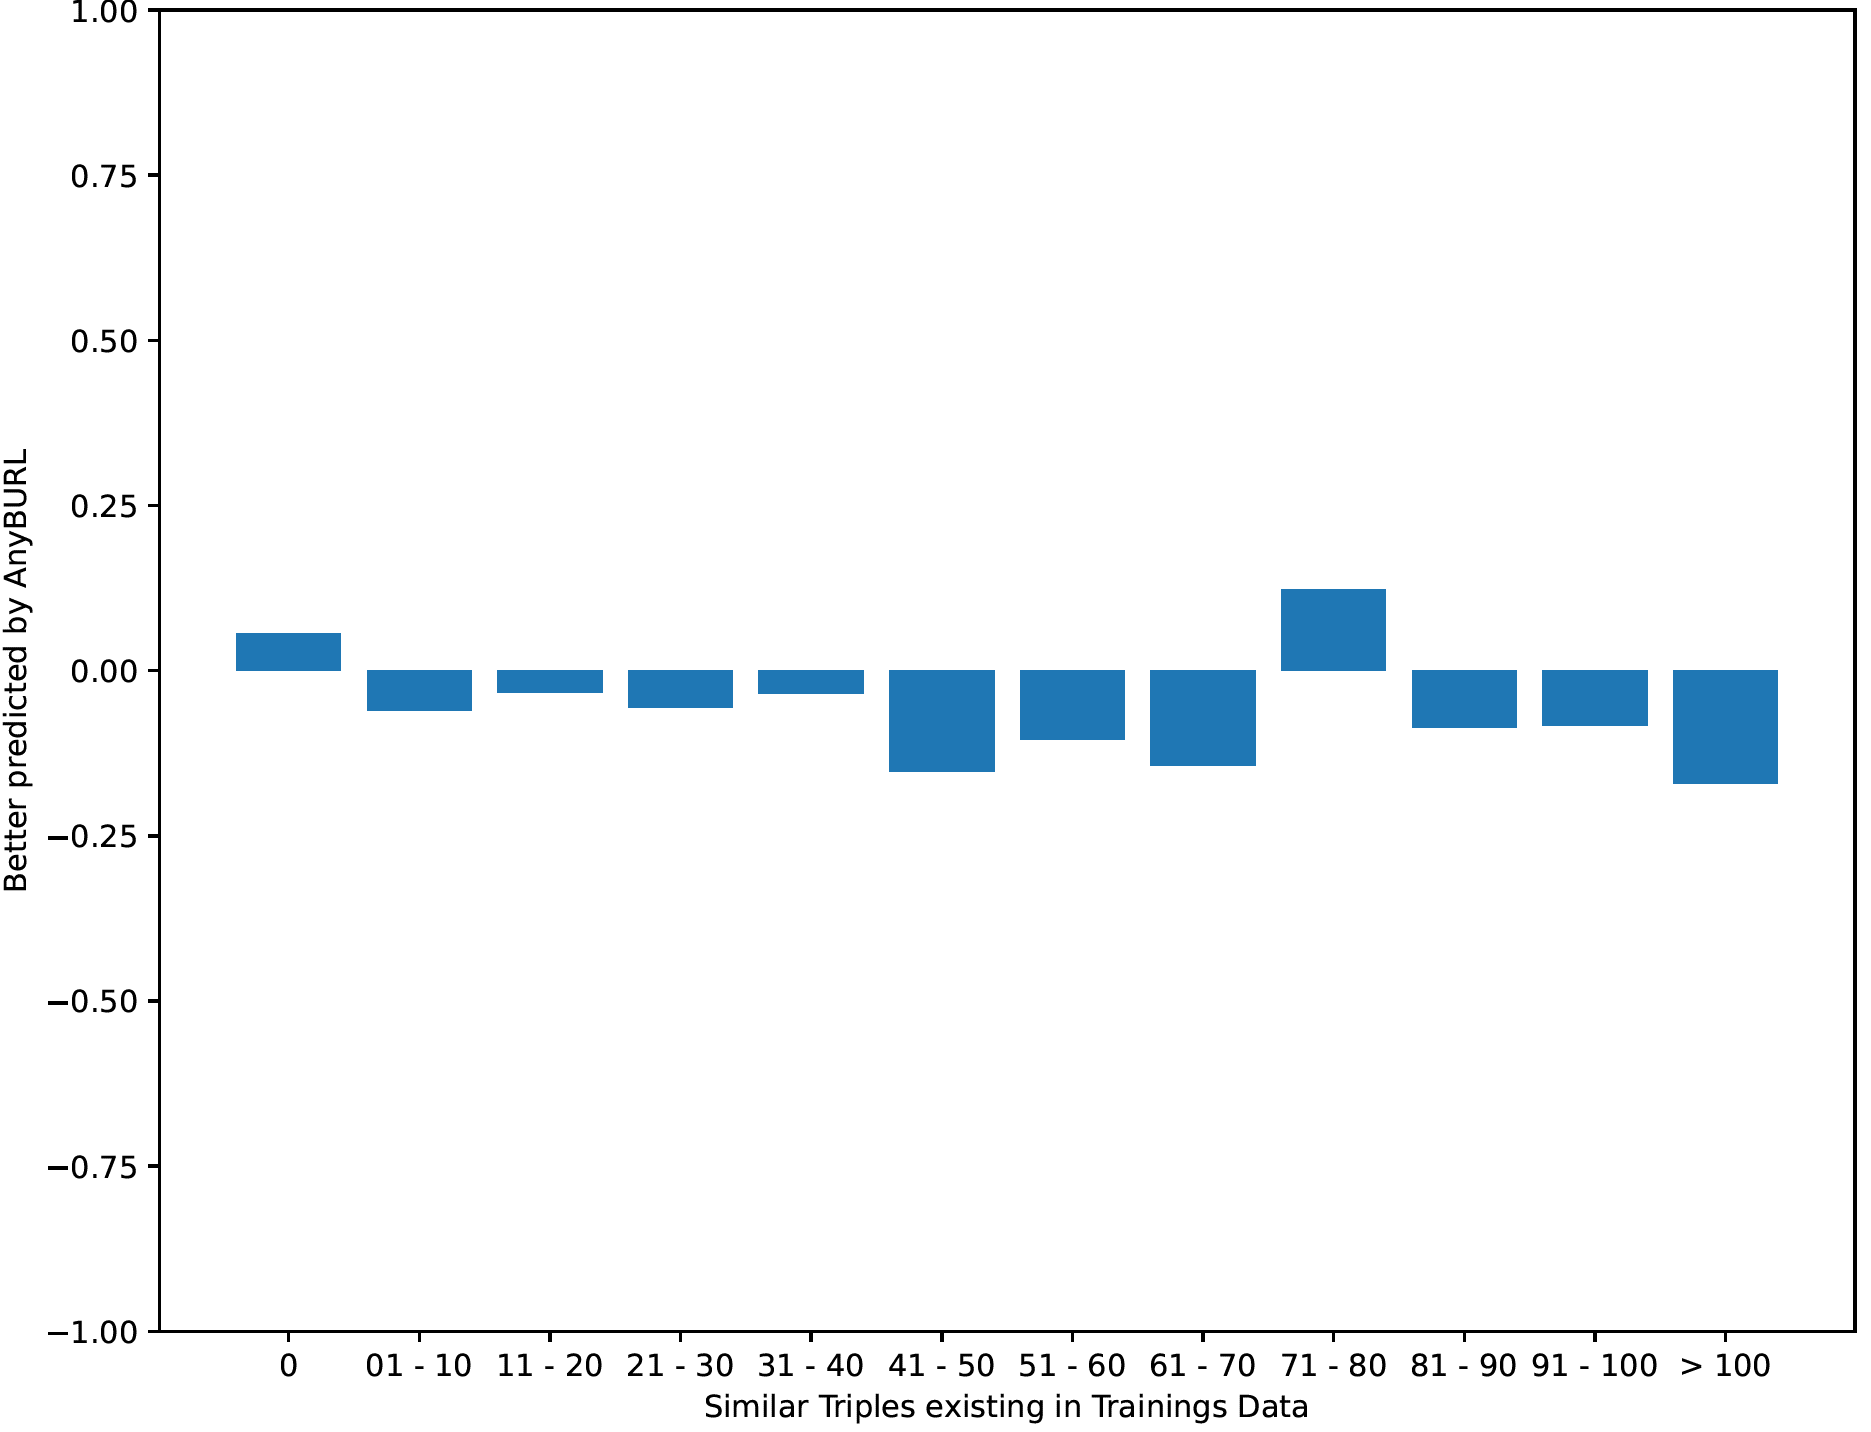
\includegraphics[width=0.7\textwidth]{images/similar_triples_steps_anyburl_rescal_codex.PNG}
\caption{Comparison of AnyBURL and RESCAL on CodEx-M in regard to the amount of similar triples in the trainings data}
\label{fig:similar_triples_steps_anyburl_rescal_codex}
\end{figure}

\begin{figure}[H]
\centering
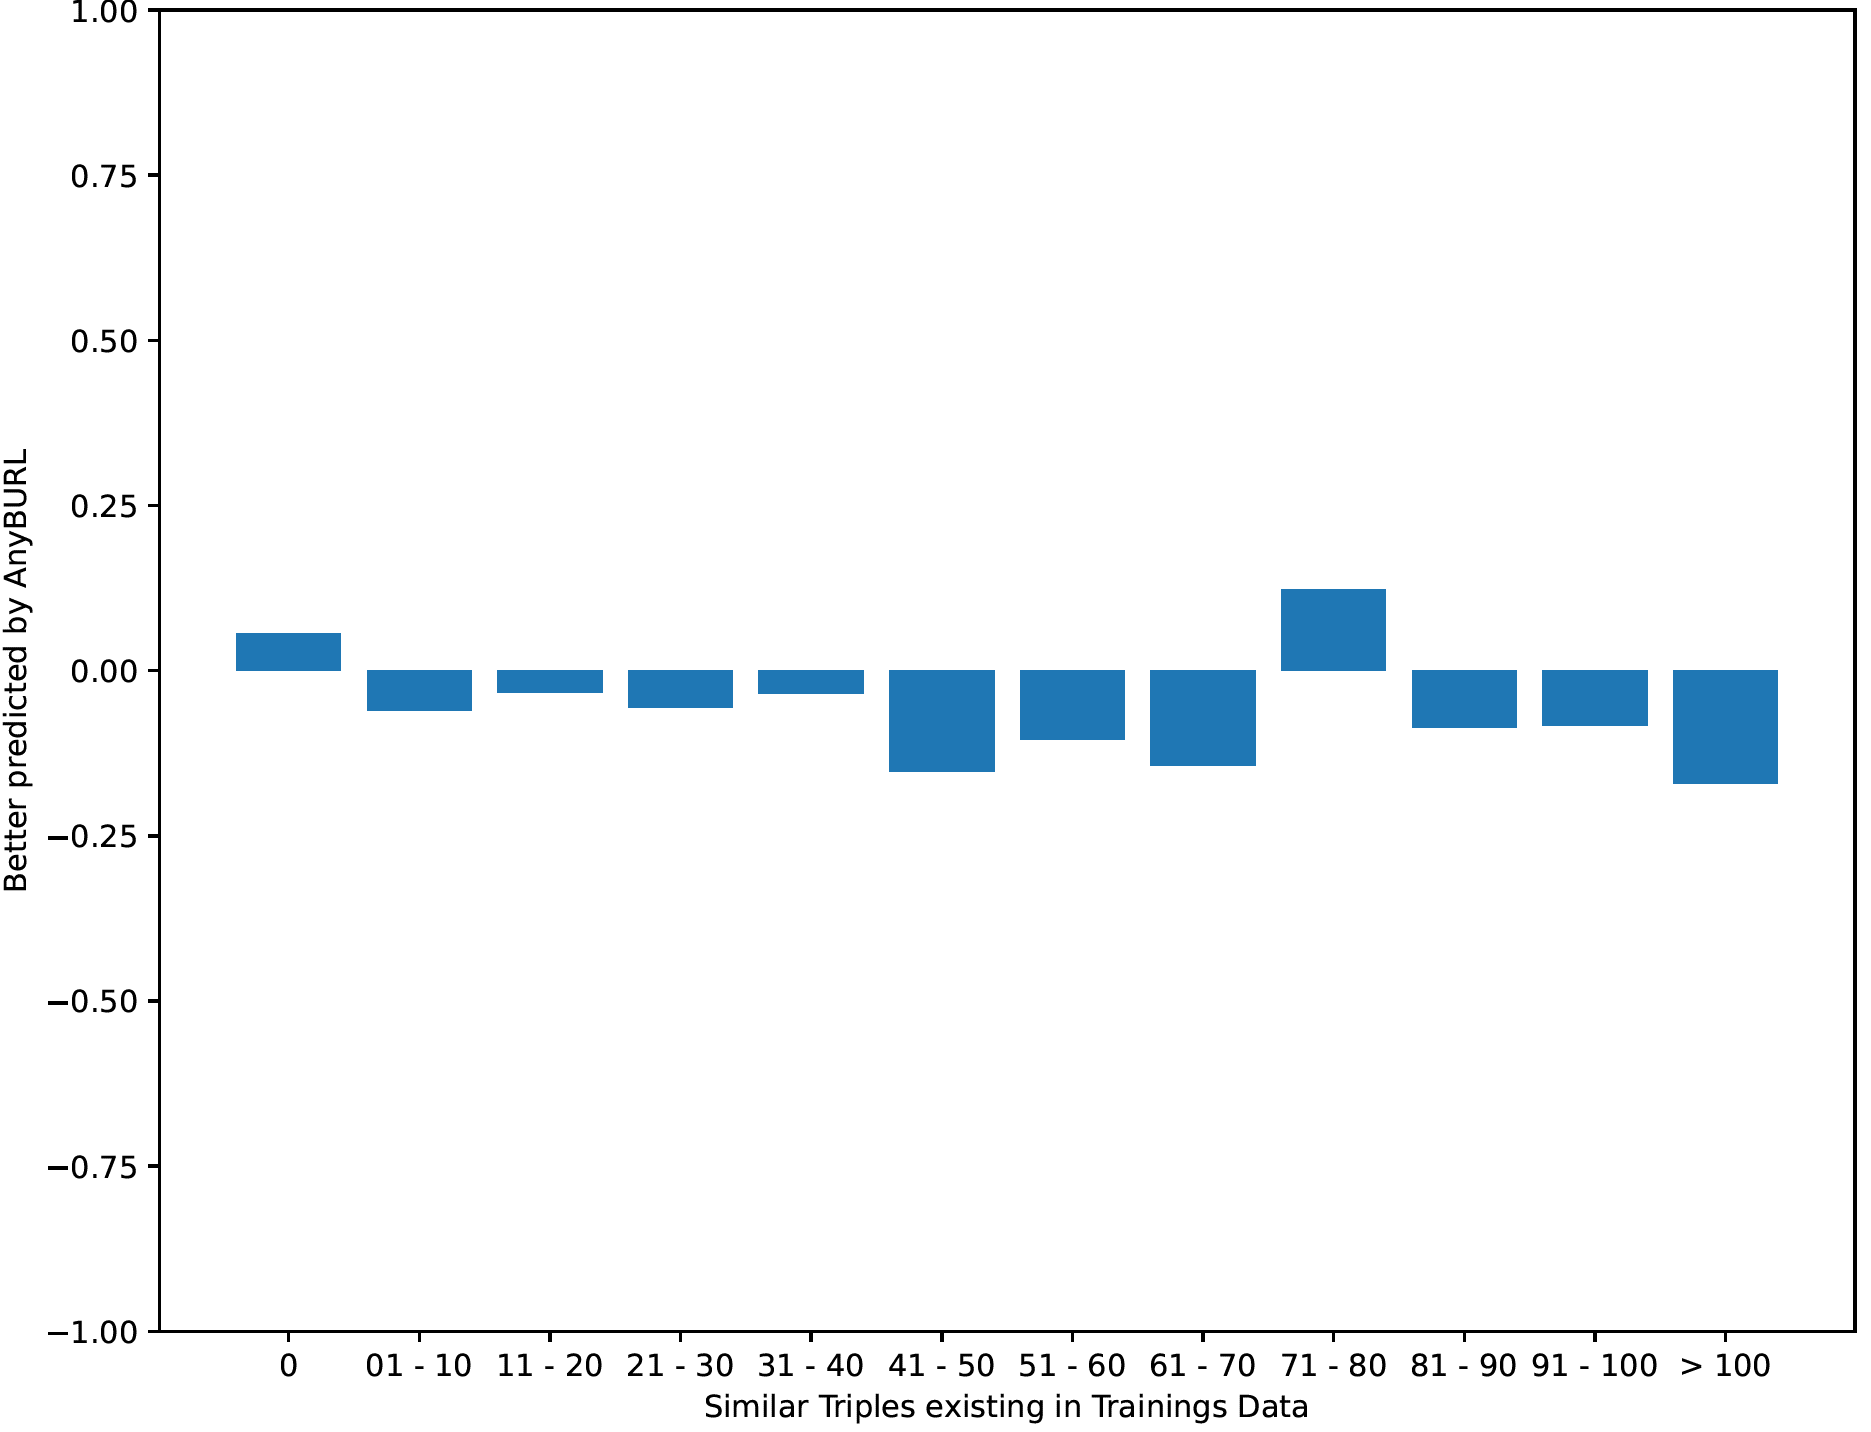
\includegraphics[width=0.7\textwidth]{images/similar_triples_steps_anyburl_complex_fb15k.PNG}
\caption{Comparison of AnyBURL and ComplEx on FB15k-237 in regard to the amount of similar triples in the trainings data}
\label{fig:similar_triples_steps_anyburl_complex_fb15k}
\end{figure}

\begin{figure}[H]
\centering
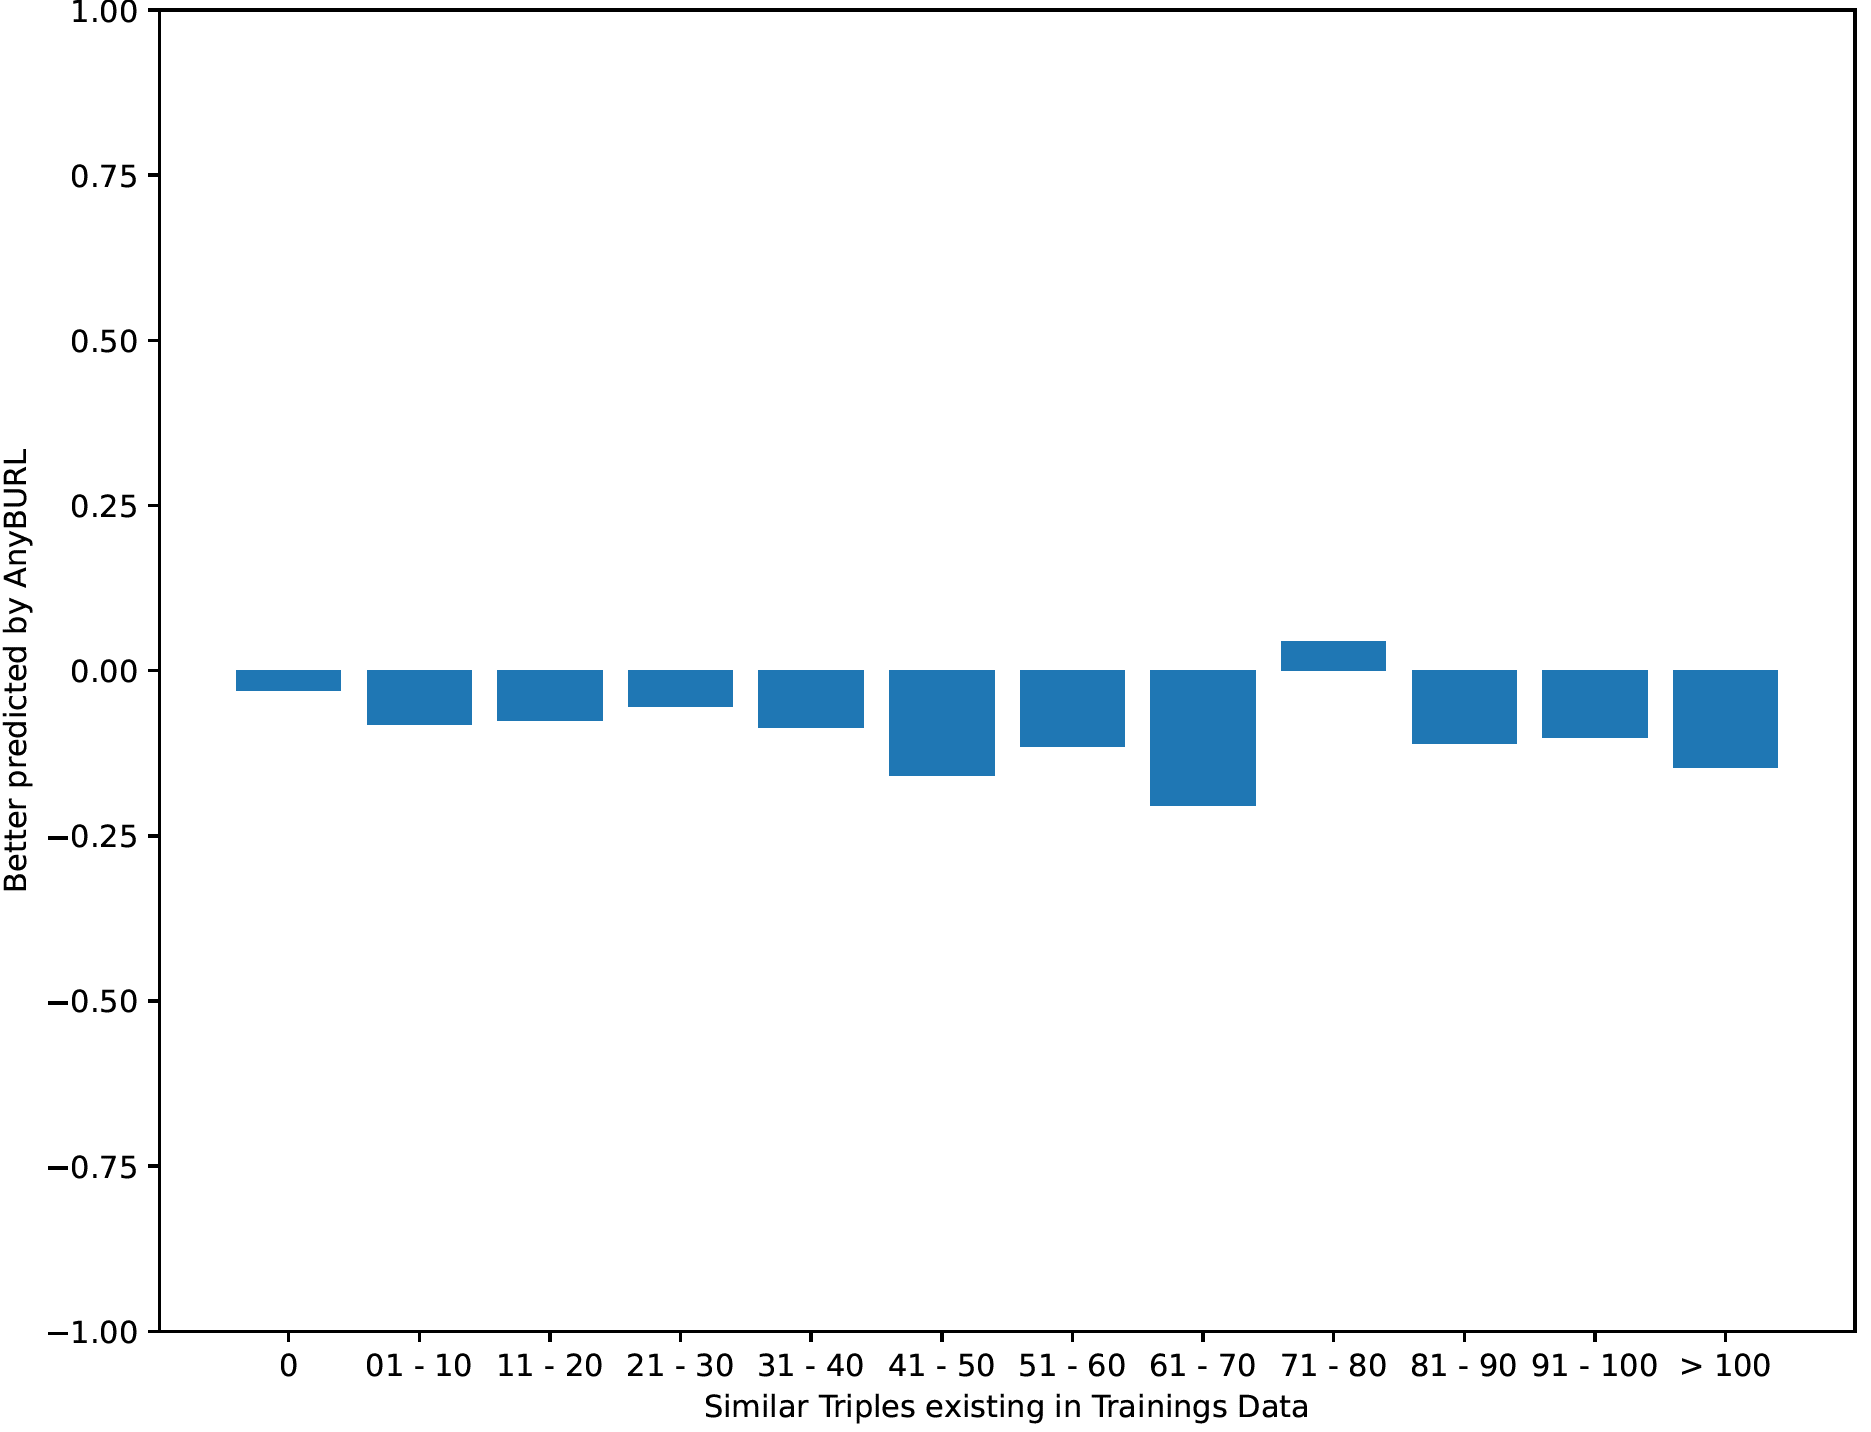
\includegraphics[width=0.7\textwidth]{images/similar_triples_steps_anyburl_conve_codex.PNG}
\caption{Comparison of AnyBURL and ConvE on FB15k-237 in regard to the amount of similar triples in the trainings data}
\label{fig:similar_triples_steps_anyburl_conve_fb15k}
\end{figure}

\begin{figure}[H]
\centering
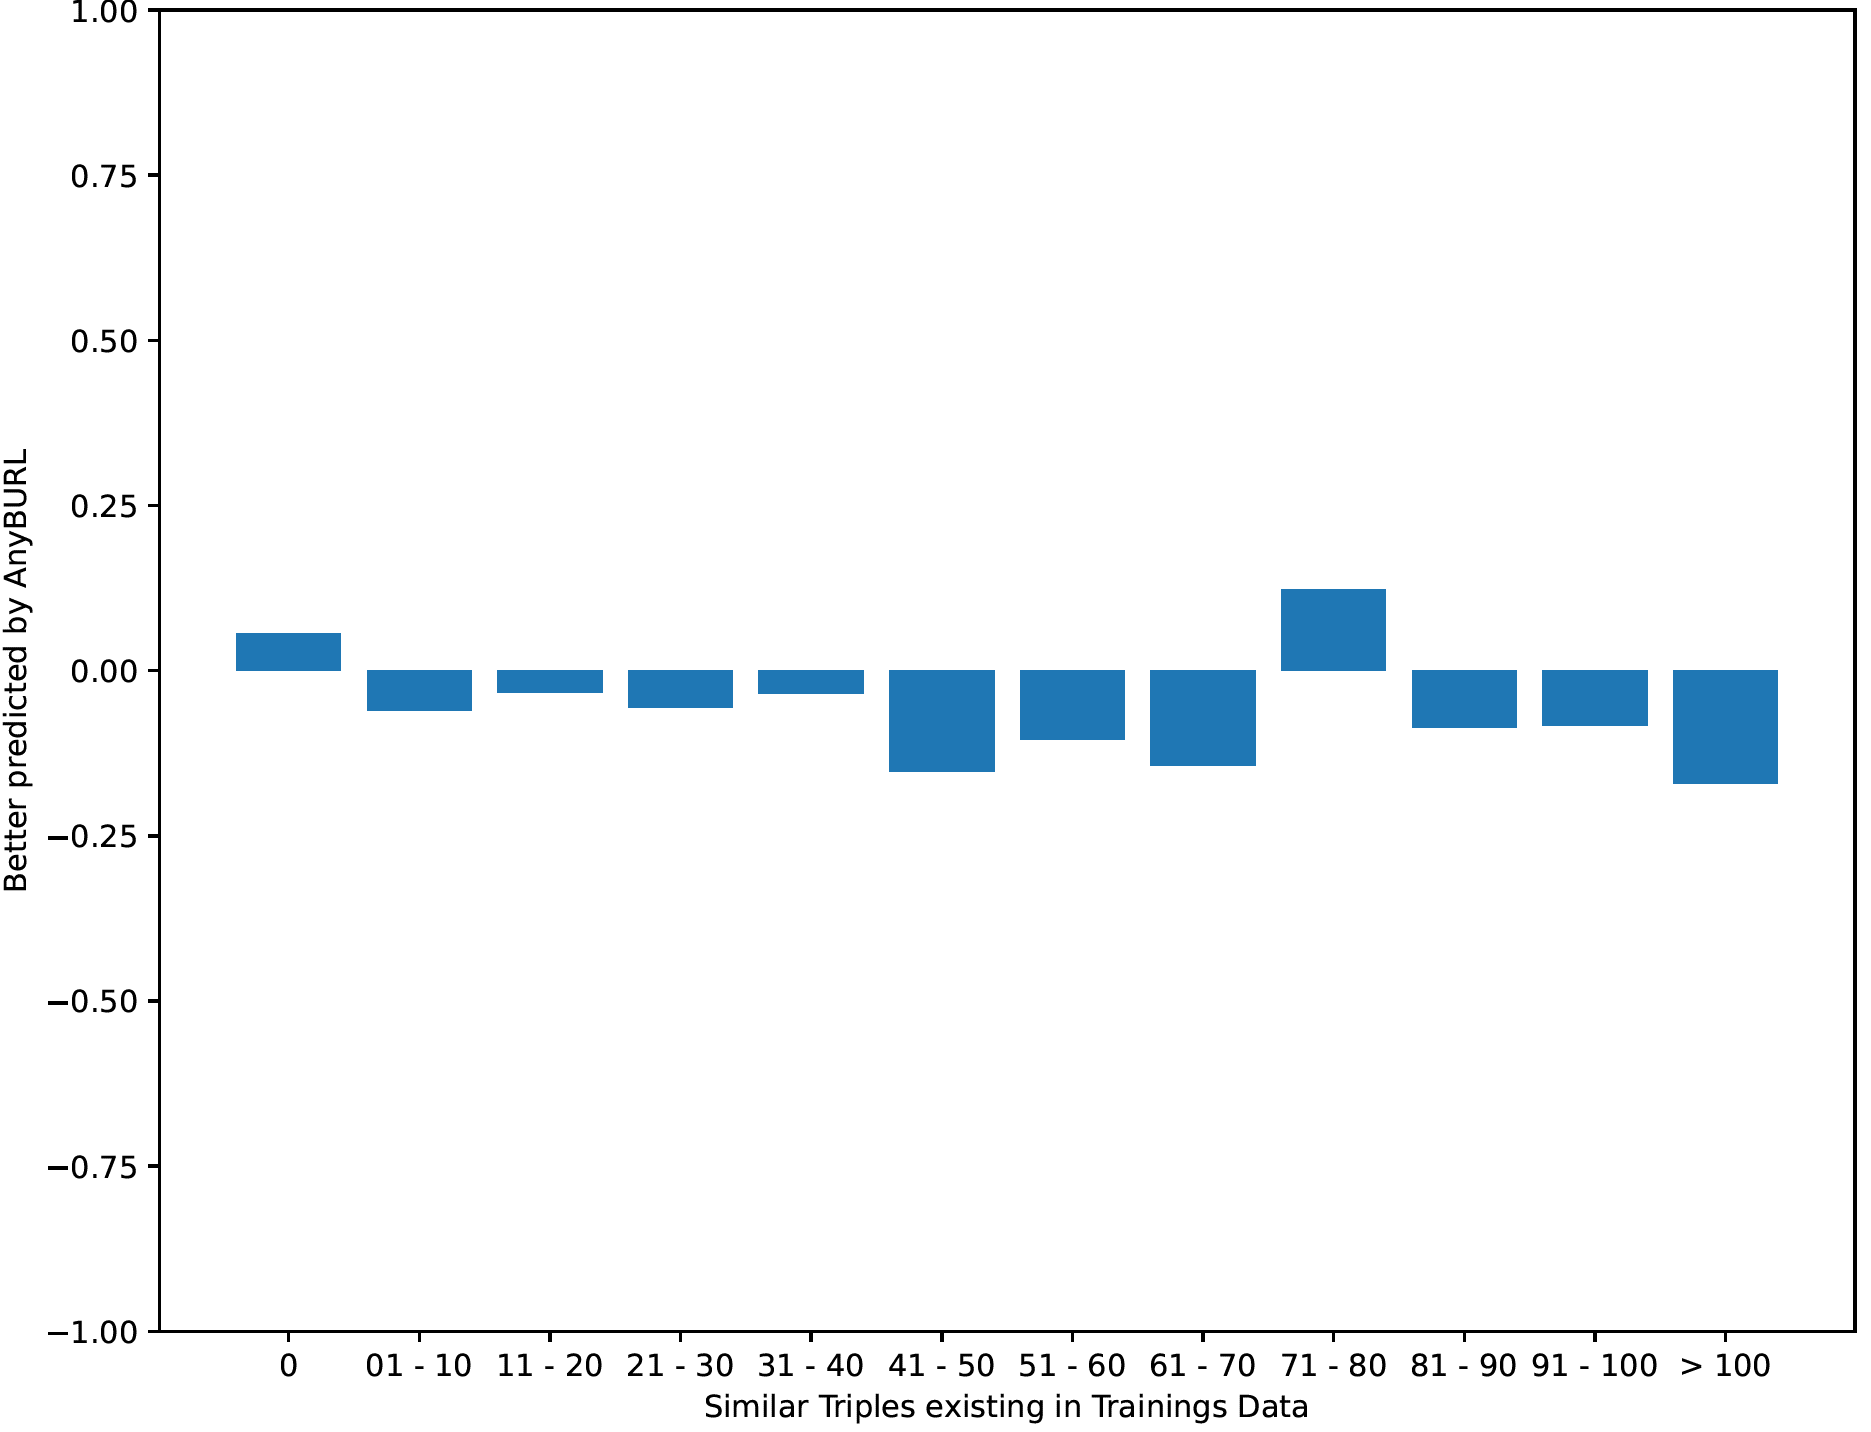
\includegraphics[width=0.7\textwidth]{images/similar_triples_steps_anyburl_rescal_codex.PNG}
\caption{Comparison of AnyBURL and RESCAL on FB15k-237 in regard to the amount of similar triples in the trainings data}
\label{fig:similar_triples_steps_anyburl_rescal_fb15k}
\end{figure}

\begin{figure}[H]
\centering
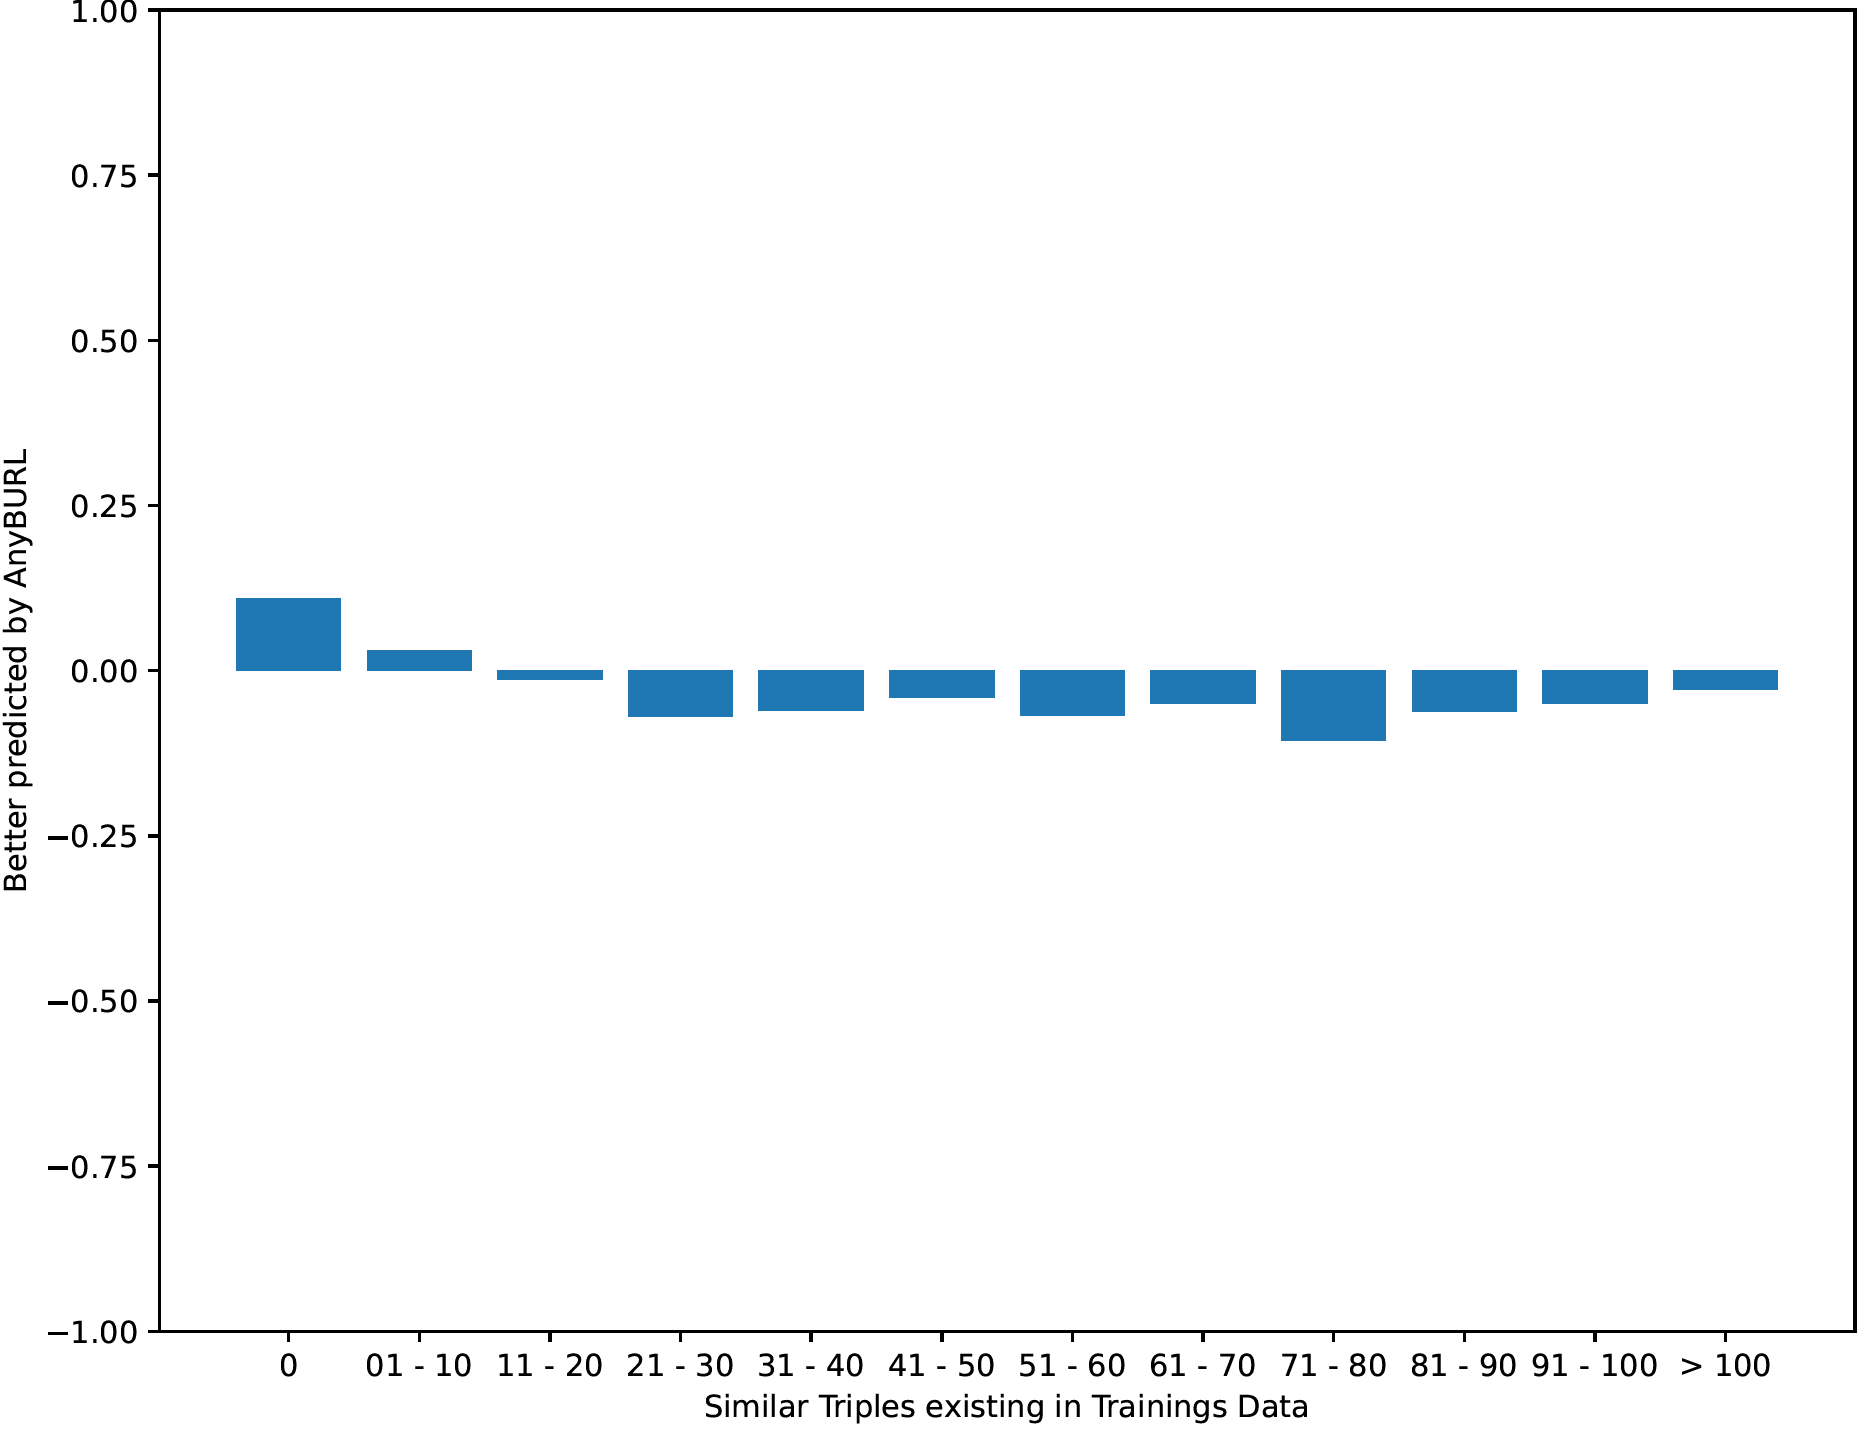
\includegraphics[width=0.7\textwidth]{images/similar_triples_steps_anyburl_complex_yago.PNG}
\caption{Comparison of AnyBURL and ComplEx on YAGO3-10 in regard to the amount of similar triples in the trainings data}
\label{fig:similar_triples_steps_anyburl_complex_yago}
\end{figure}


\section{Comparison in regard to the existence of Similar Entities}
\label{appendix:similar_entities}
\subsection{AnyBURL and ComplEx on CoDEx-M}

\begin{figure}[H]
\centering
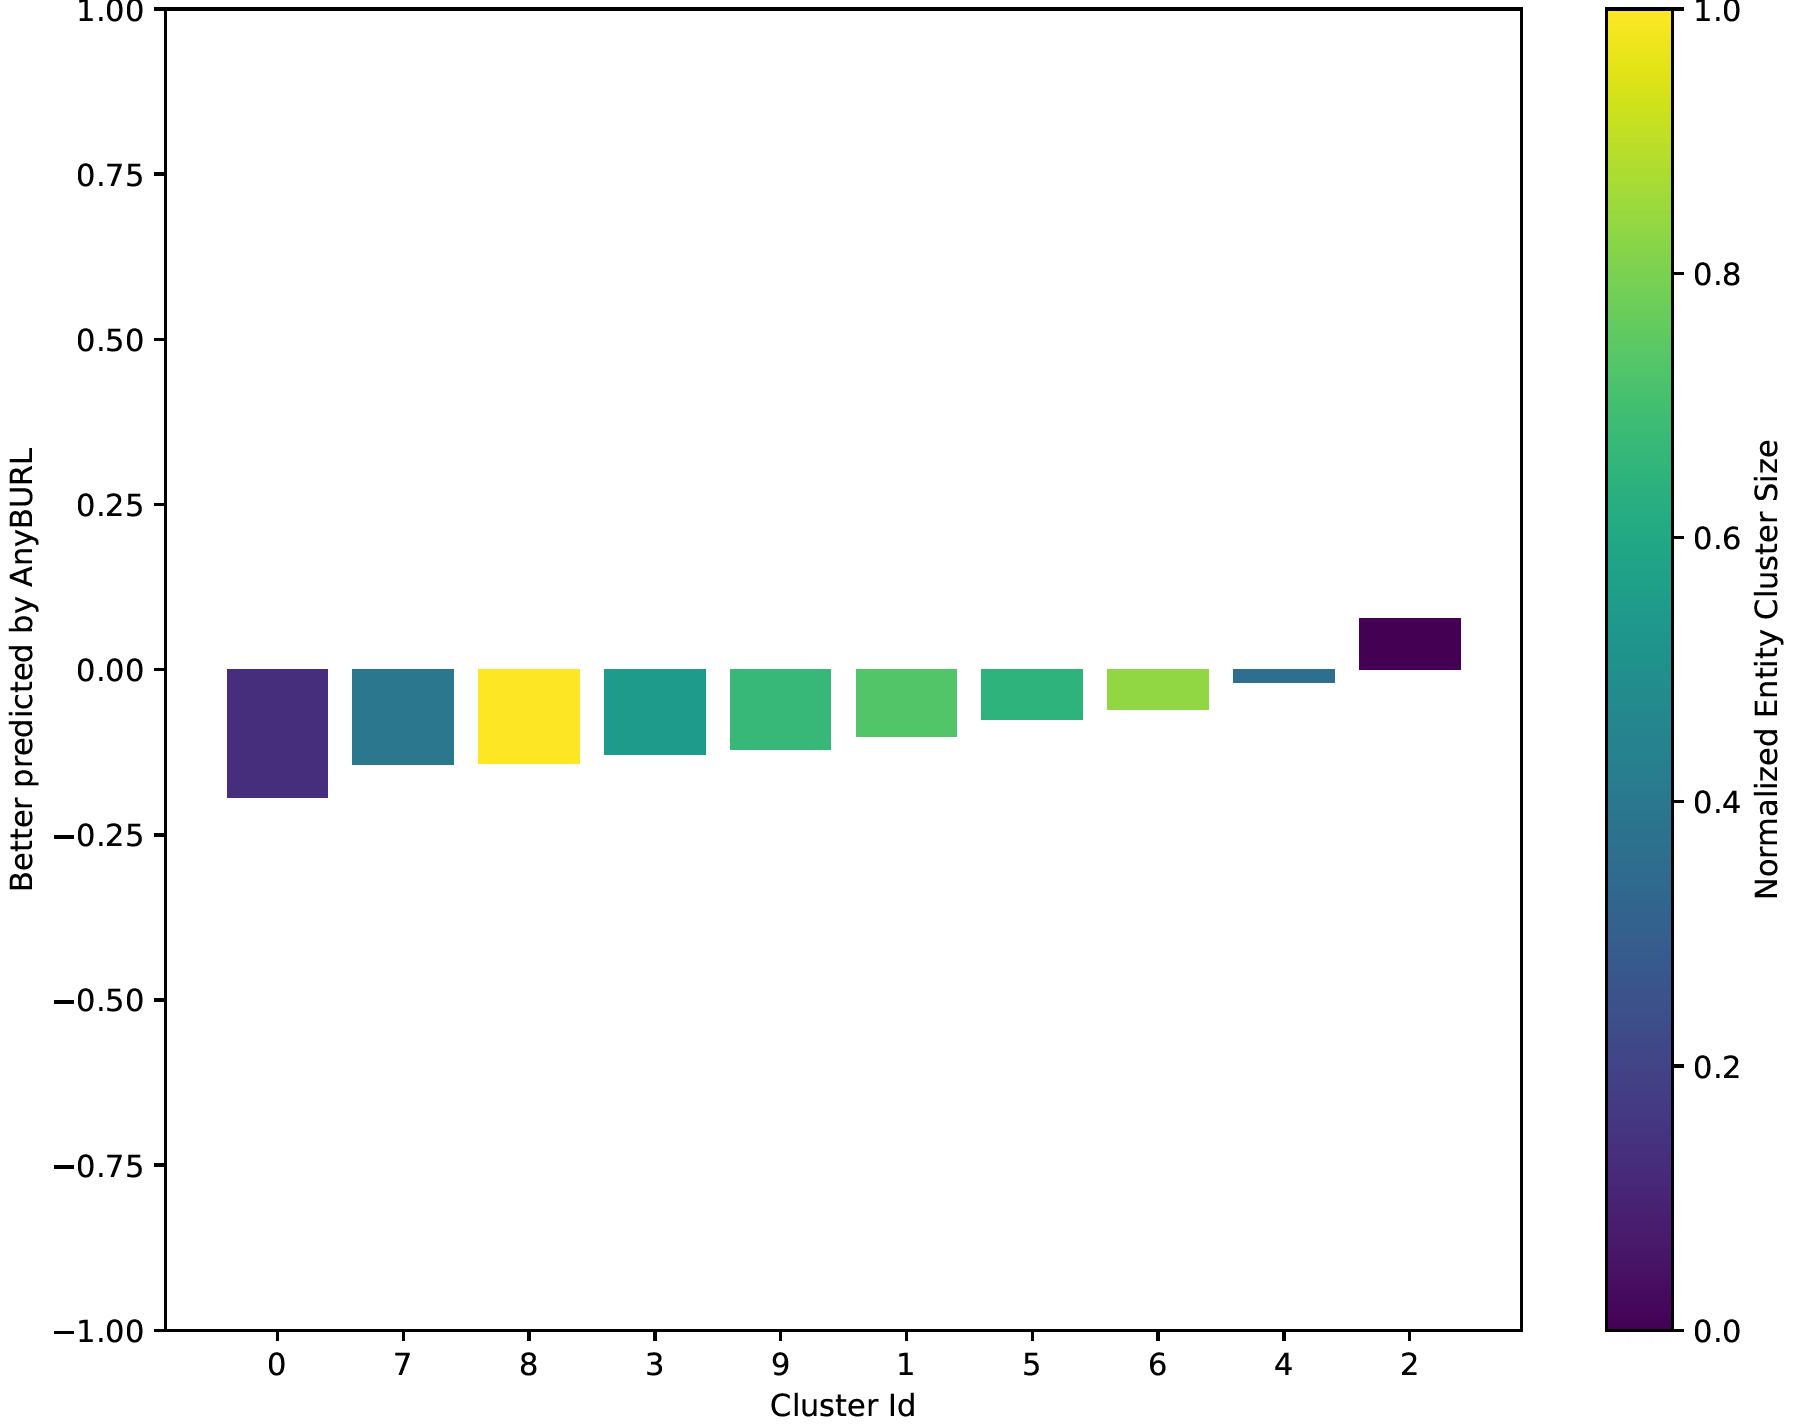
\includegraphics[width=0.7\textwidth]{images/head_cluster_10_anyburl_complex_codex.PNG}
\caption{Comparison of AnyBURL and ComplEx on CoDEx-M in regard to the existence of similar head entities based on K-Means Clustering (k=10)}
\label{fig:head_cluster_10_anyburl_complex_codex}
\end{figure}

\begin{figure}[H]
\centering
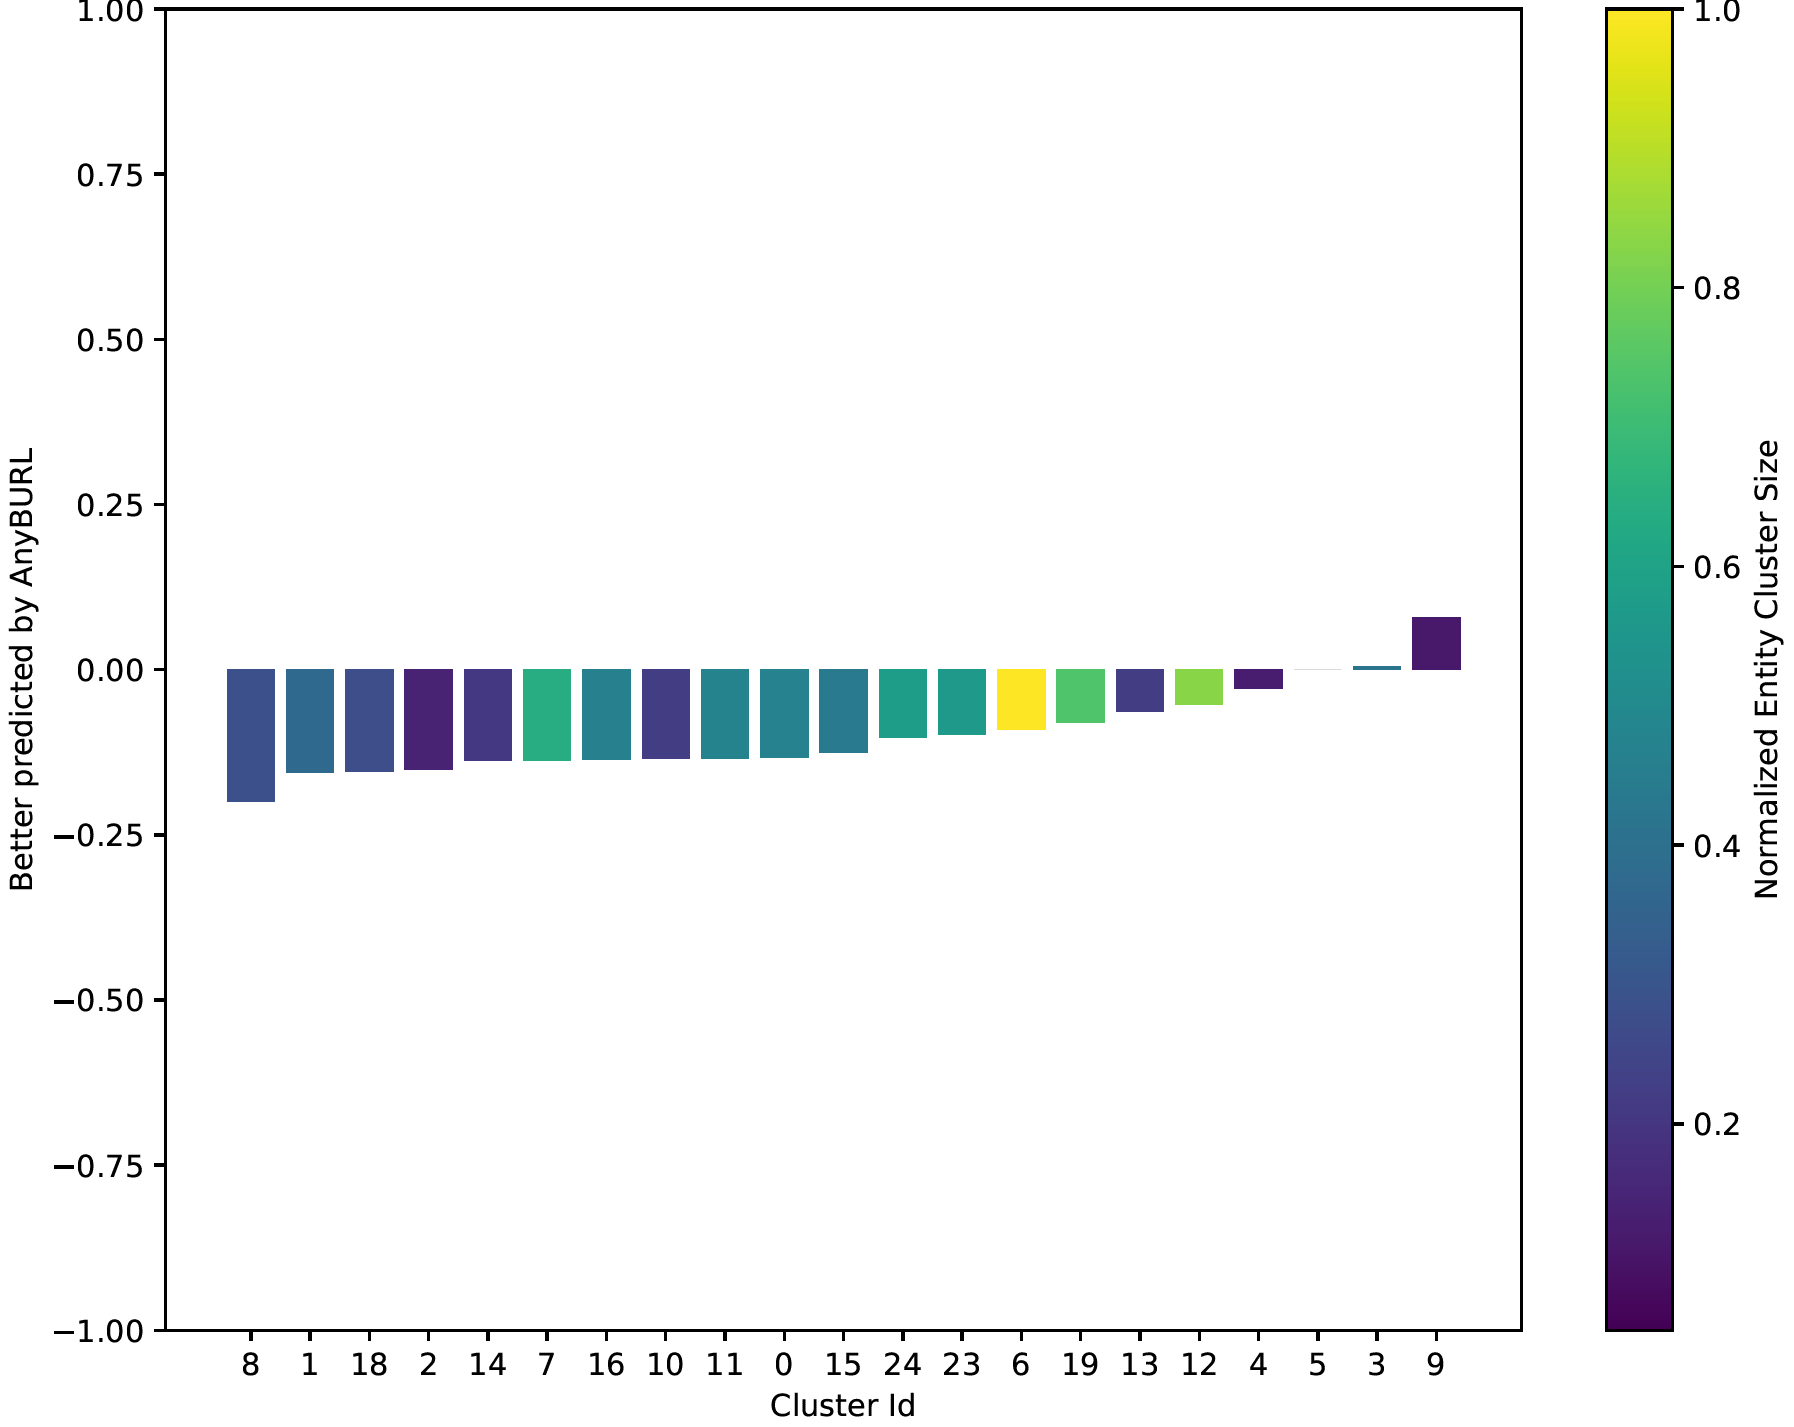
\includegraphics[width=0.7\textwidth]{images/head_cluster_25_anyburl_complex_codex.PNG}
\caption{Comparison of AnyBURL and ComplEx on CoDEx-M in regard to the existence of similar head entities based on K-Means Clustering (k=25)}
\label{fig:head_cluster_25_anyburl_complex_codex}
\end{figure}

\begin{figure}[H]
\centering
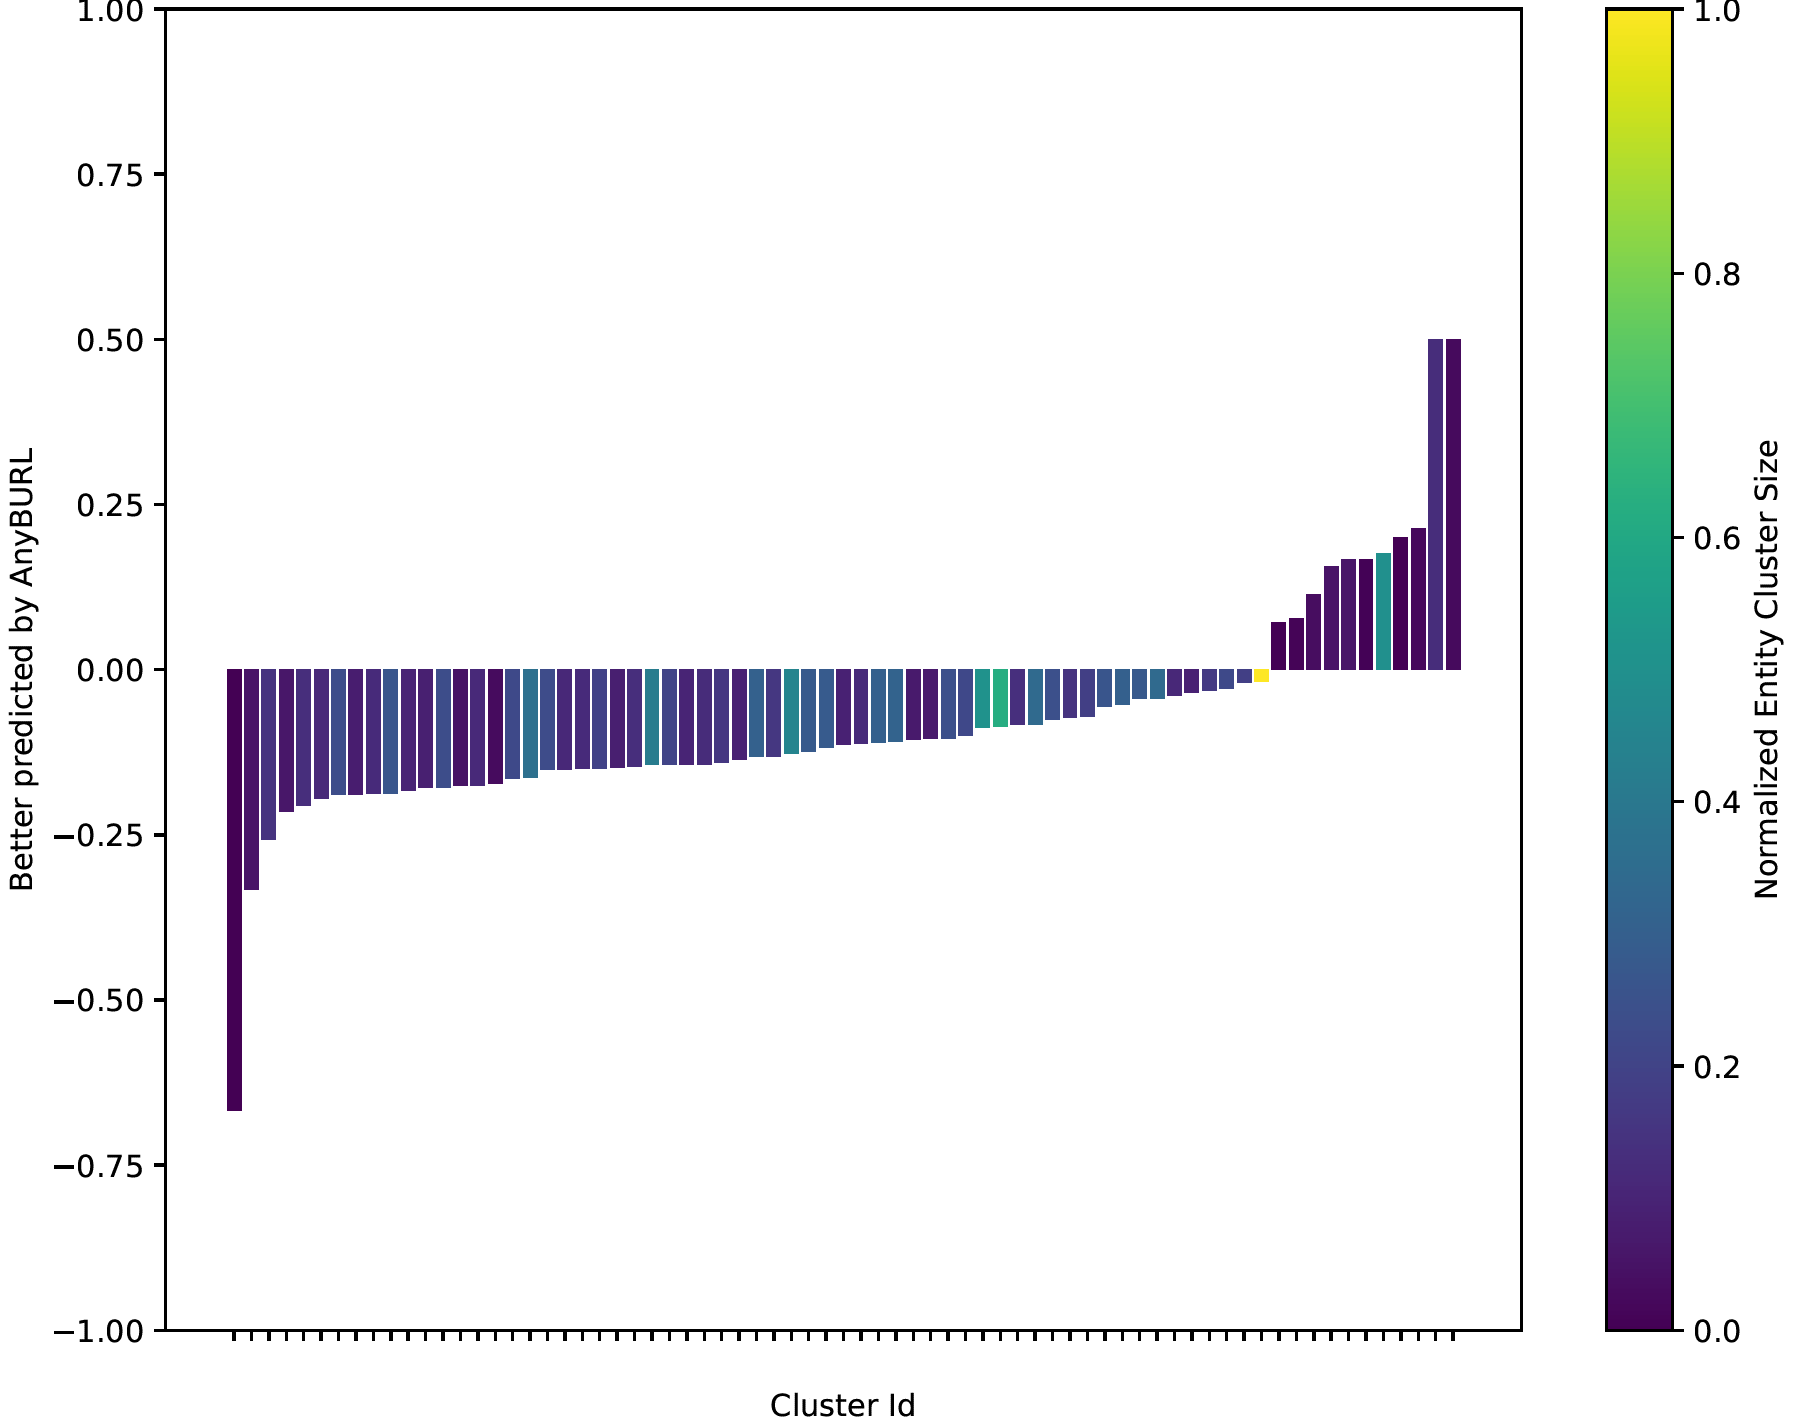
\includegraphics[width=0.7\textwidth]{images/head_cluster_100_anyburl_complex_codex.PNG}
\caption{Comparison of AnyBURL and ComplEx on CoDEx-M in regard to the existence of similar head entities based on K-Means Clustering (k=100)}
\label{fig:head_cluster_100_anyburl_complex_codex}
\end{figure}

\begin{figure}[H]
\centering
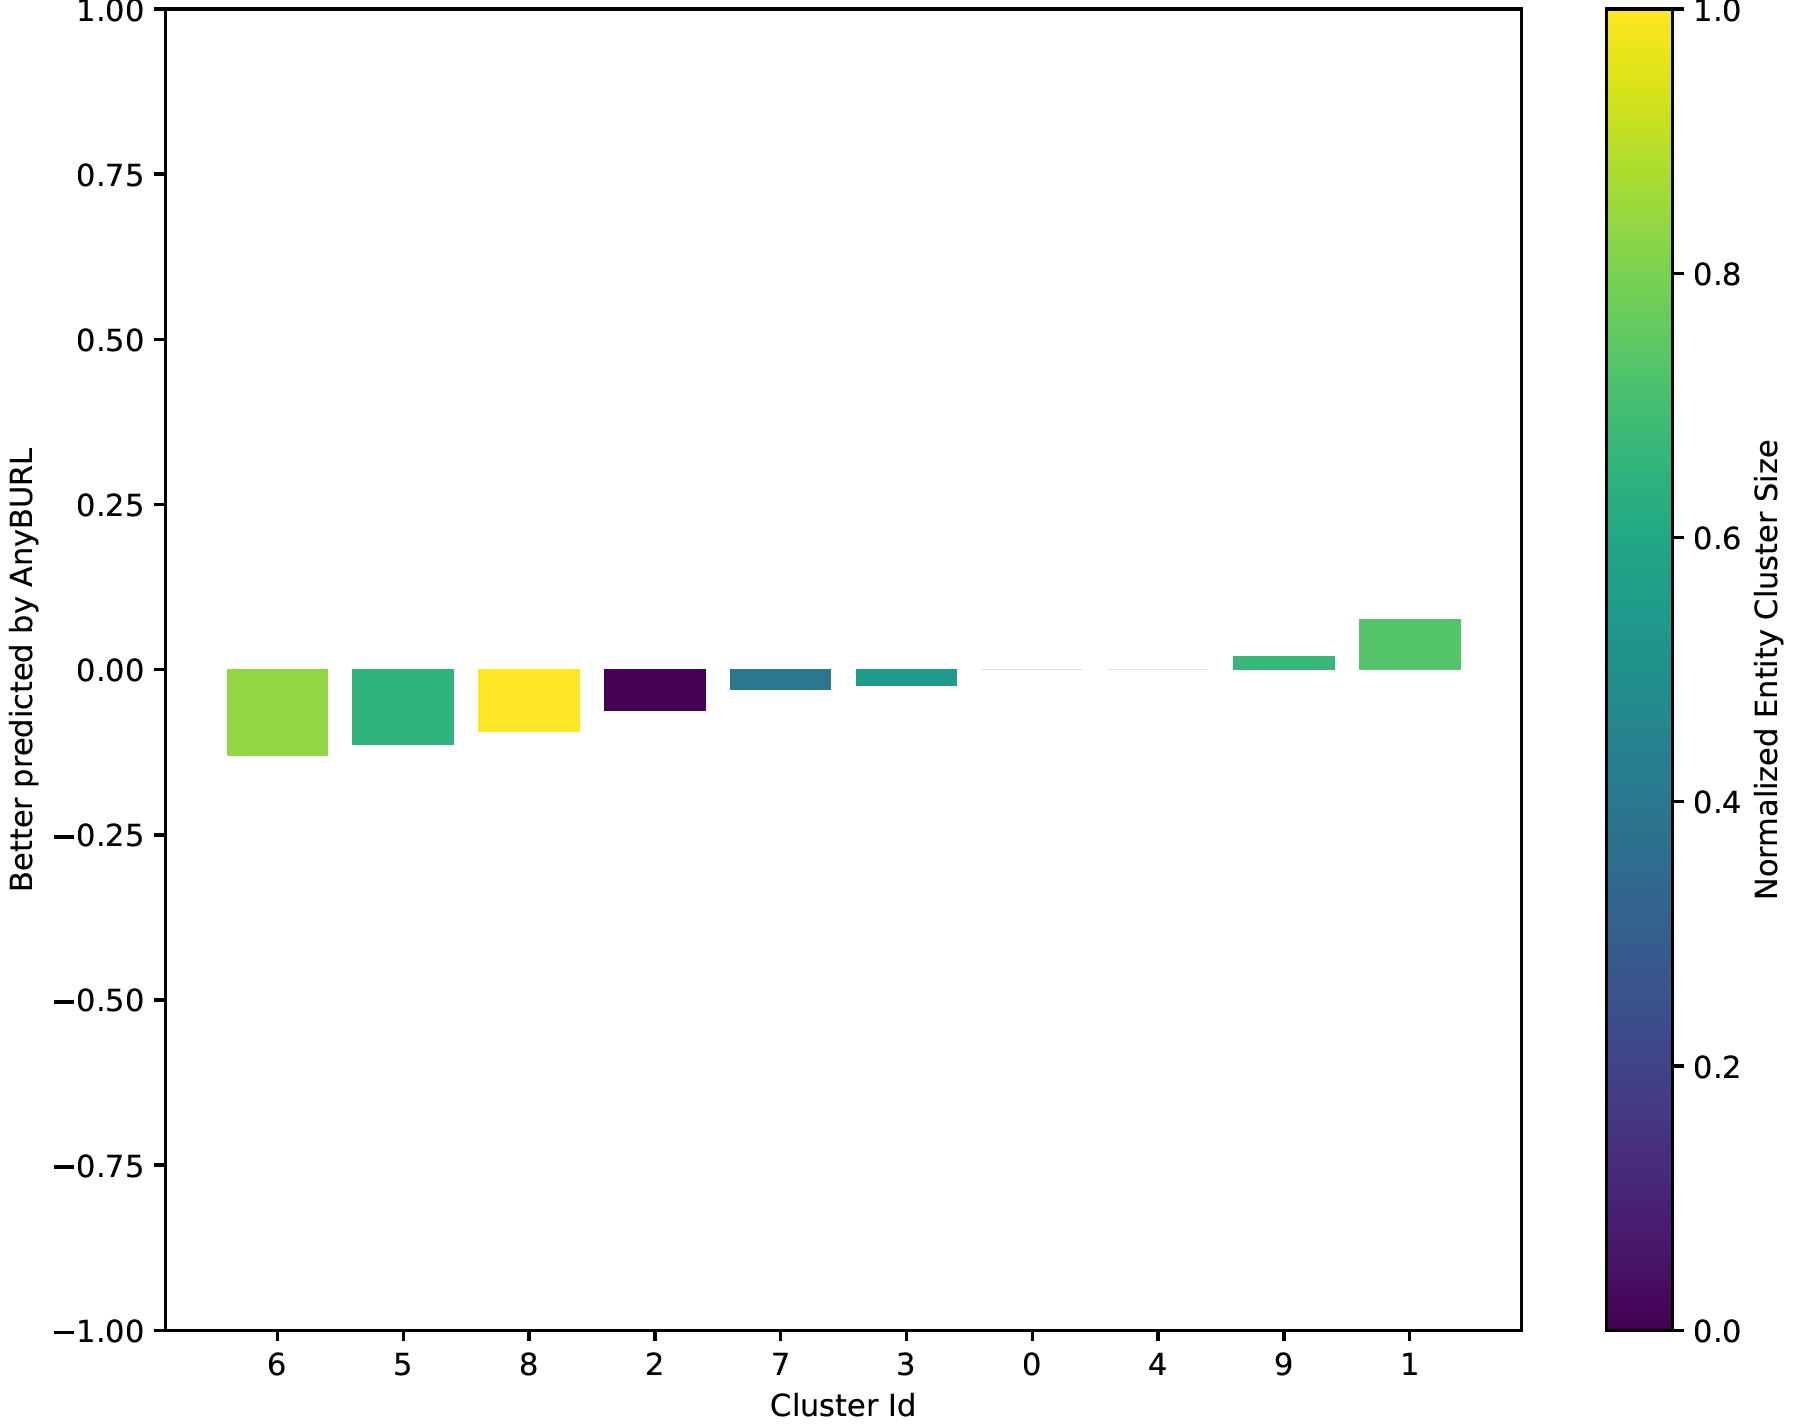
\includegraphics[width=0.7\textwidth]{images/tail_cluster_10_anyburl_complex_codex.PNG}
\caption{Comparison of AnyBURL and ComplEx on CoDEx-M in regard to the existence of similar tail entities based on K-Means Clustering (k=10)}
\label{fig:tail_cluster_10_anyburl_complex_codex}
\end{figure}

\begin{figure}[H]
\centering
\includegraphics[width=0.7\textwidth]{images/tail_cluster_25_anyburl_complex_codex.PNG}
\caption{Comparison of AnyBURL and ComplEx on CoDEx-M in regard to the existence of similar tail entities based on K-Means Clustering (k=25)}
\label{fig:tail_cluster_25_anyburl_complex_codex}
\end{figure}



\subsection{AnyBURL and ConvE on CoDEx-M}

\begin{figure}[H]
\centering
\includegraphics[width=0.7\textwidth]{images/head_cluster_100_anyburl_conve_codex.PNG}
\caption{Comparison of AnyBURL and ConvE on CoDEx-M in regard to the existence of similar head entities based on K-Means Clustering (k=100)}
\label{fig:head_cluster_100_anyburl_conve_codex}
\end{figure}


\subsection{AnyBURL and RESCAL on CoDEx-M}

\begin{figure}[H]
\centering
\includegraphics[width=0.7\textwidth]{images/head_cluster_100_anyburl_rescal_codex.PNG}
\caption{Comparison of AnyBURL and ConvE on CoDEx-M in regard to the existence of similar head entities based on K-Means Clustering (k=100)}
\label{fig:head_cluster_100_anyburl_rescal_codex}
\end{figure}

\subsection{AnyBURL and ComplEx on FB15k-237}

\begin{figure}[H]
\centering
\includegraphics[width=0.7\textwidth]{images/head_cluster_100_anyburl_complex_fb15k.PNG}
\caption{Comparison of AnyBURL and ComplEx on FB15k-237 in regard to the existence of similar head entities based on K-Means Clustering (k=100)}
\label{fig:head_cluster_100_anyburl_complex_fb15k}
\end{figure}

\subsection{AnyBURL and ConvE on FB15k-237}

\begin{figure}[H]
\centering
\includegraphics[width=0.7\textwidth]{images/head_cluster_100_anyburl_conve_fb15k.PNG}
\caption{Comparison of AnyBURL and ConvE on FB15k-237 in regard to the existence of similar head entities based on K-Means Clustering (k=100)}
\label{fig:head_cluster_100_anyburl_conve_fb15k}
\end{figure}

\begin{figure}[H]
\centering
\includegraphics[width=0.7\textwidth]{images/tail_cluster_100_anyburl_conve_fb15k.PNG}
\caption{Comparison of AnyBURL and ConvE on FB15k-237 in regard to the existence of similar tail entities based on K-Means Clustering (k=100)}
\label{fig:tail_cluster_100_anyburl_conve_fb15k}
\end{figure}

\subsection{AnyBURL and RESCAL on FB15k-237}

\begin{figure}[H]
\centering
\includegraphics[width=0.7\textwidth]{images/head_cluster_100_anyburl_rescal_fb15k.PNG}
\caption{Comparison of AnyBURL and RESCAL on FB15k-237 in regard to the existence of similar head entities based on K-Means Clustering (k=100)}
\label{fig:head_cluster_100_anyburl_rescal_fb15k}
\end{figure}

\begin{figure}[H]
\centering
\includegraphics[width=0.7\textwidth]{images/tail_cluster_100_anyburl_rescal_fb15k.PNG}
\caption{Comparison of AnyBURL and RESCAL on FB15k-237 in regard to the existence of similar tail entities based on K-Means Clustering (k=100)}
\label{fig:tail_cluster_100_anyburl_rescal_fb15k}
\end{figure}

\subsection{AnyBURL and ComplEx on YAGO3-10}

\begin{figure}[H]
\centering
\includegraphics[width=0.7\textwidth]{images/head_cluster_100_anyburl_complex_yago.PNG}
\caption{Comparison of AnyBURL and ComplEx on YAGO3-10 in regard to the existence of similar head entities based on K-Means Clustering (k=100)}
\label{fig:head_cluster_100_anyburl_complex_yago}
\end{figure}


\newpage


\pagestyle{empty}


\section*{Ehrenw\"ortliche Erkl\"arung}
Ich versichere, dass ich die beiliegende Master-/Bachelorarbeit ohne Hilfe Dritter
und ohne Benutzung anderer als der angegebenen Quellen und Hilfsmittel
angefertigt und die den benutzten Quellen w\"ortlich oder inhaltlich
entnommenen Stellen als solche kenntlich gemacht habe. Diese Arbeit
hat in gleicher oder \"ahnlicher Form noch keiner Pr\"ufungsbeh\"orde
vorgelegen. Ich bin mir bewusst, dass eine falsche Erkl\"arung rechtliche Folgen haben
wird.
\\
\\

\noindent
Mannheim, den 31.08.2022 \hspace{4cm} Unterschrift

\end{document}
